\documentclass[a4paper,12pt]{article}

% Работа с русским языком
\usepackage{cmap}					          % поиск в PDF
\usepackage{mathtext} 				        % русские буквы в фомулах
\usepackage[T2A]{fontenc}		         % кодировка
\usepackage[utf8]{inputenc}			     % кодировка исходного текста
\usepackage[english,russian]{babel}	% локализация и переносы

% Работа с картинками
\usepackage{graphicx}  	   % Для вставки рисунков
\graphicspath{{images/}}  % папки с картинками
 
\usepackage{ulem}

\usepackage{hyperref}
\usepackage[usenames,dvipsnames,svgnames,table,rgb]{xcolor}
\hypersetup{				                                  % Гиперссылки
	unicode=true,                                            % русские буквы в раздела PDF
	pdftitle={Заголовок},                                % Заголовок
	pdfauthor={Автор},                                   % Автор
	pdfsubject={Тема},                                    % Тема
	pdfcreator={Создатель},                          % Создатель
	pdfproducer={Производитель},              % Производитель
	pdfkeywords={keyword1} {key2} {key3}, % Ключевые слова
	colorlinks=true,       	                                 % false: ссылки в рамках; true: цветные ссылки
	linkcolor=red,                                            % внутренние ссылки
	citecolor=green,                                        % на библиографию
	filecolor=magenta,                                    % на файлы
	urlcolor=blue                                             % на URL
}

\begin{document} 	  % конец преамбулы, начало документа

\thispagestyle{empty}
\begin{center}
	\textit{spol. s r.o.}
	\vspace{0.5ex}
	
	\textbf{VÝSOKÁ ŠKOLA HOTELOVÁ V PRAZE}
\end{center}
\vspace{13ex}

\begin{center}
	\vspace{13ex}
	\textbf{ИНФОРМАЦИОННАЯ СИСТЕМА VŠH}
	\vspace{1ex}
	
	\textbf{\textit{<<Краткое пособие>>}}
	
	\vfill
	
\includegraphics[width=0.5\textwidth]{logo}
	
	\vfill
	Прага 2014
\end{center}

\newpage

\section{Введение}

Данное пособие создано для того, чтобы помочь новым студентам VŠH ориентироваться в \sout{этой бездне ужаса и ада}
информационной системе школы и быть хорошо информированным студентом.

Этот документ не является официальным и сделан исключительно ради прикола и веселья.

\vspace{15ex}
\textbf{Let's ROLL!}

\newpage

\section{Вход в систему}

Чтобы зайти в информационную систему VŠH, необходимо набрать 
в строке браузера следующий адрес: \url{http://is.vsh.cz/}
Там вы увидите такую картину:

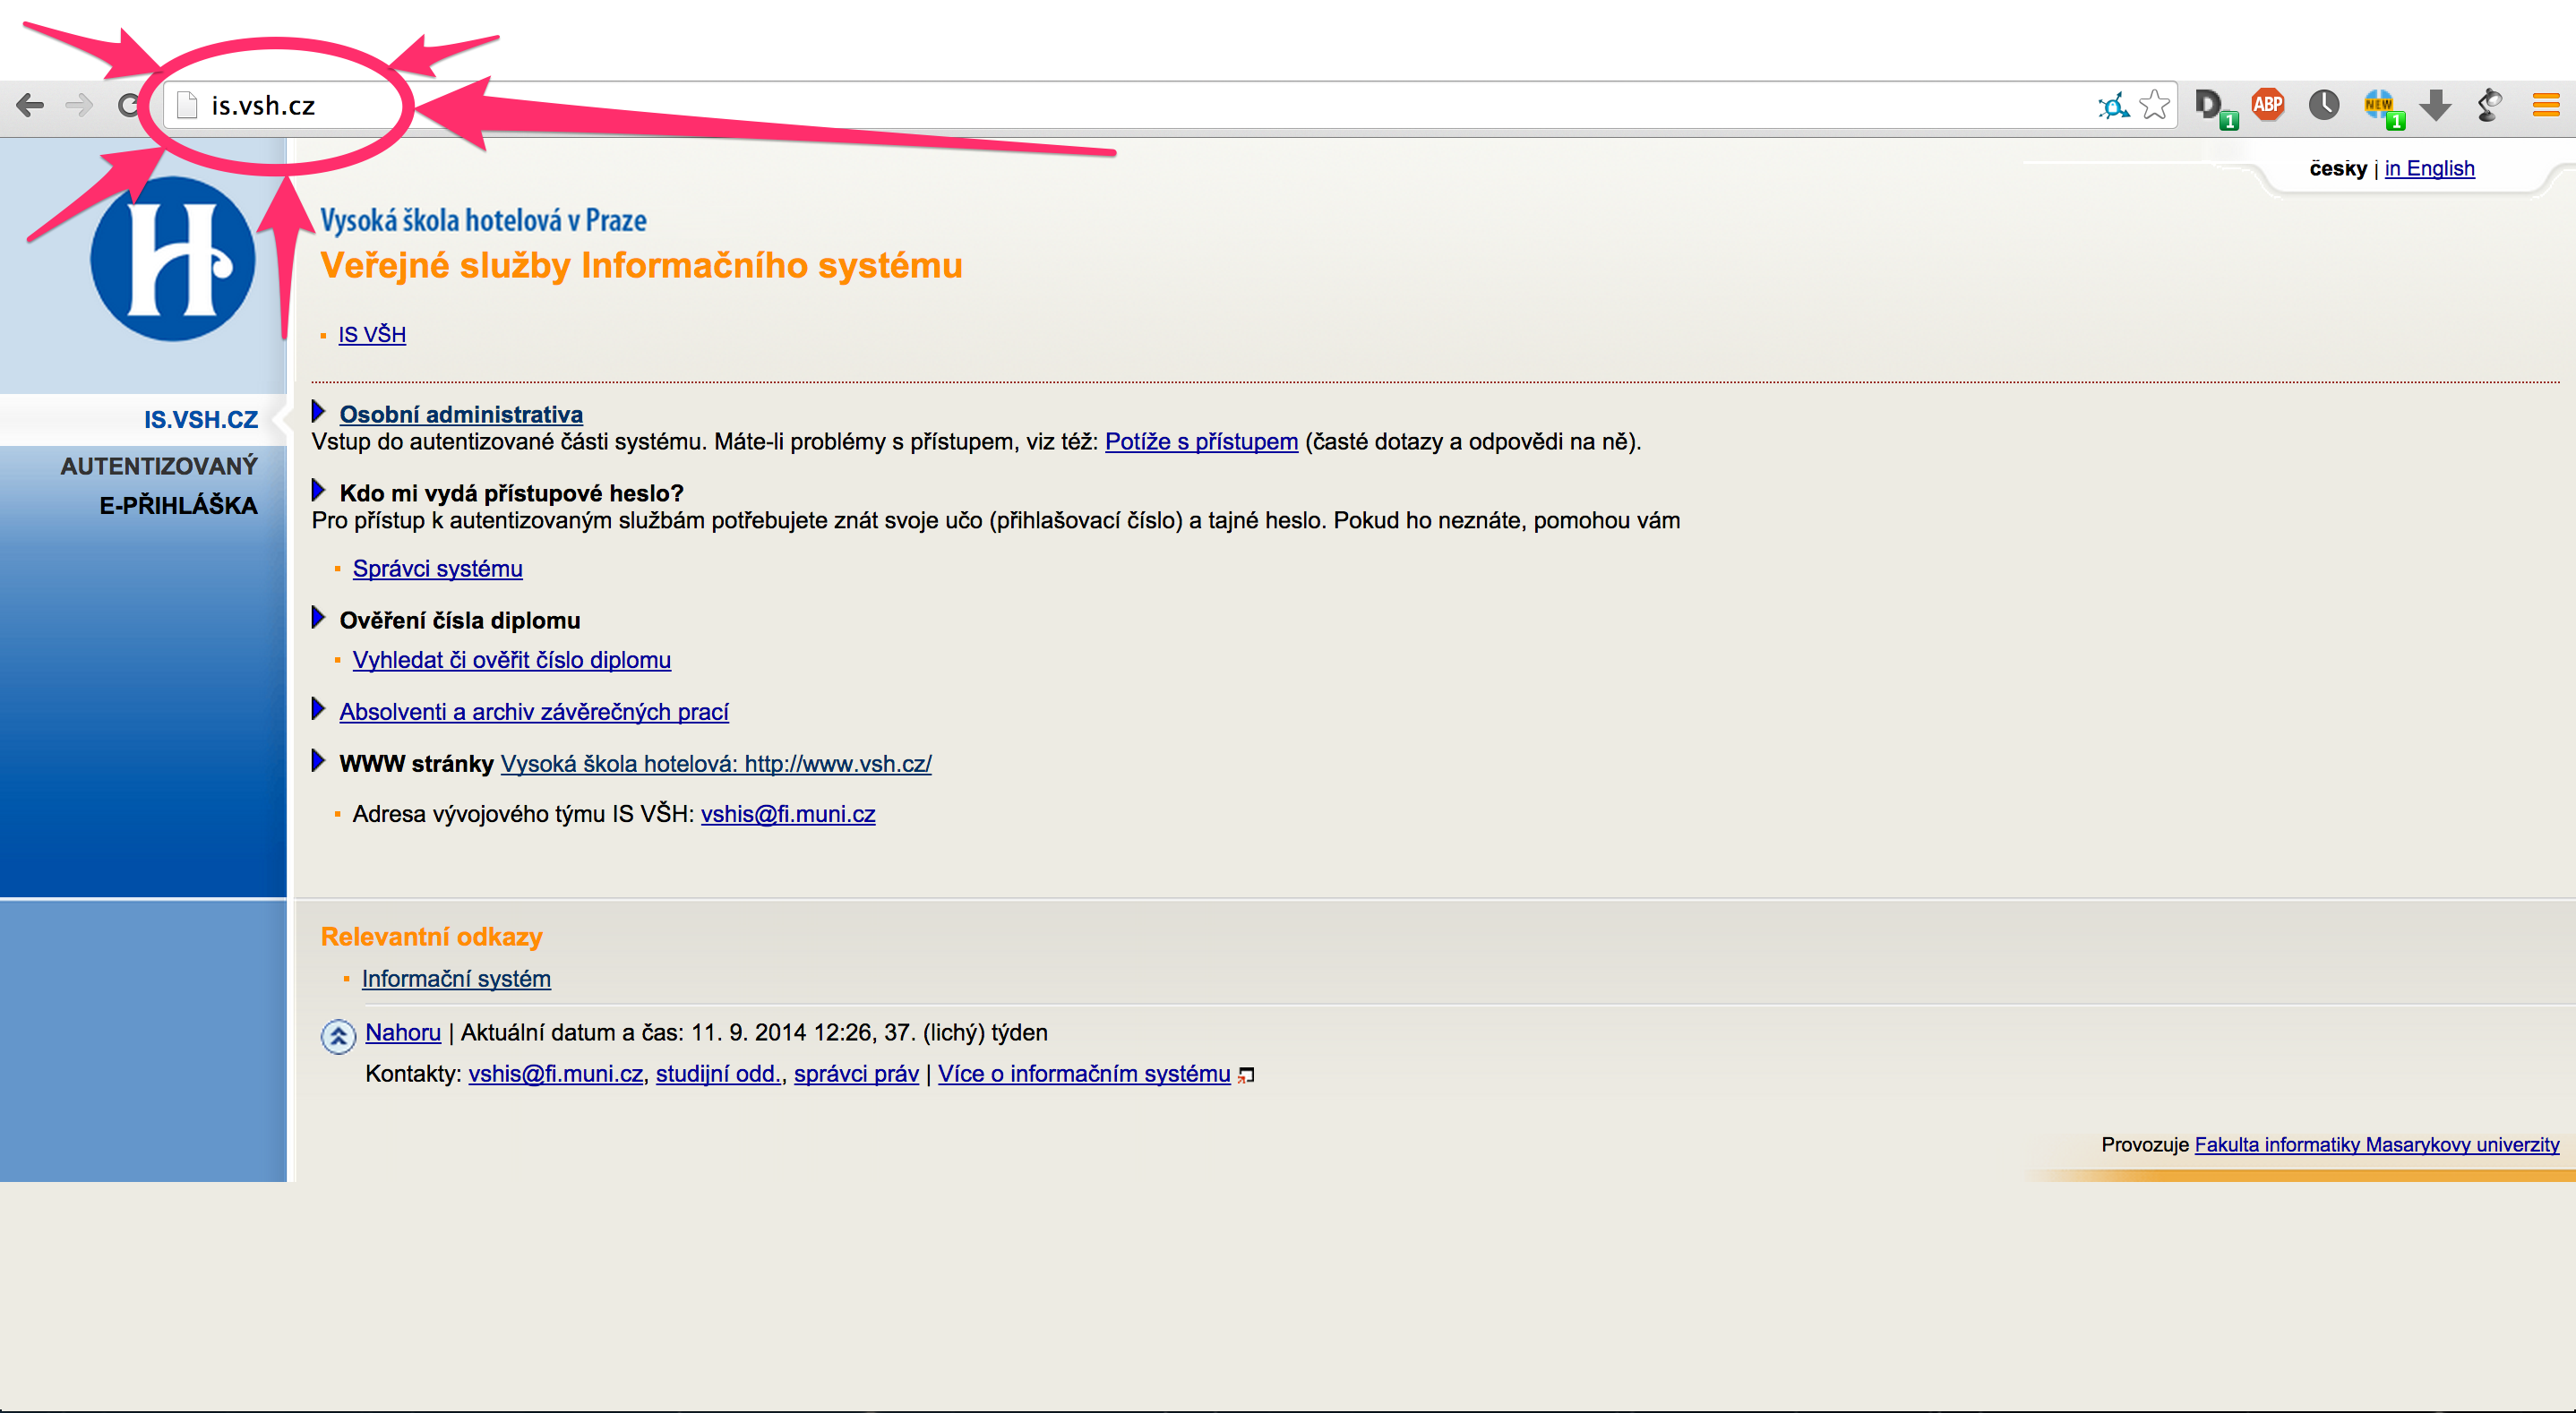
\includegraphics[width=\textwidth]{s01} \\

Теперь необходимо нажать на кнопку \href{http://is.vsh.cz/auth}{AUTENTIZOVANÝ} \\

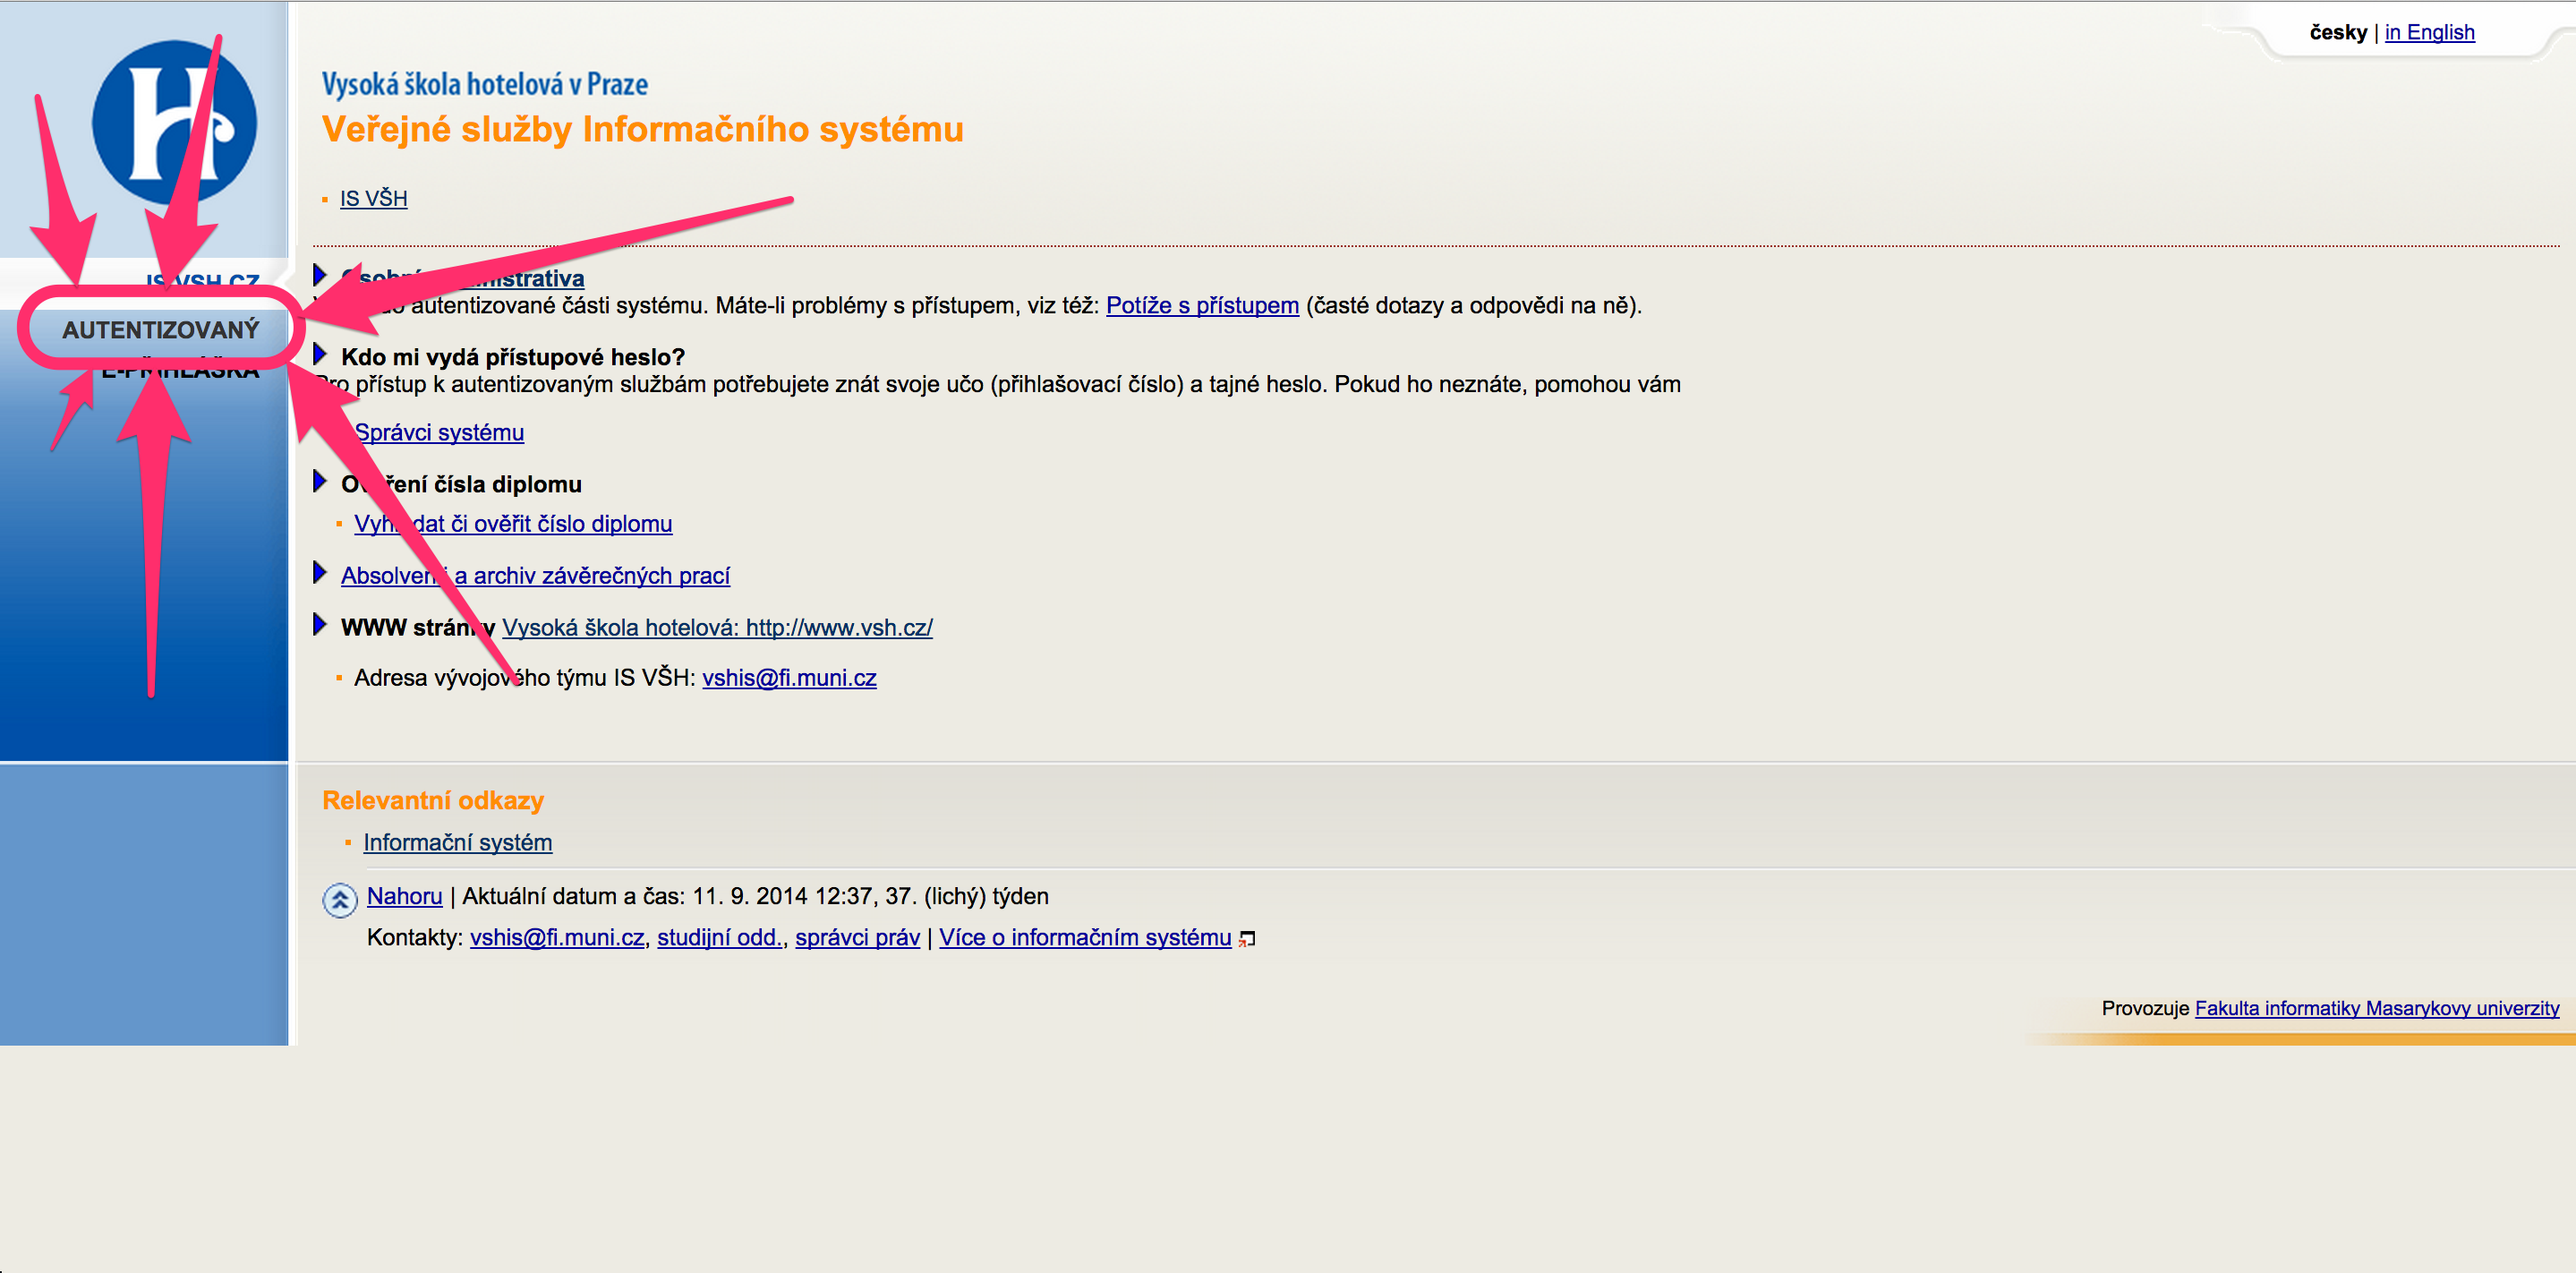
\includegraphics[width=\textwidth]{s02} \\

\newpage

Далее вы попадаете на страницу ввода логина и пароля. \\

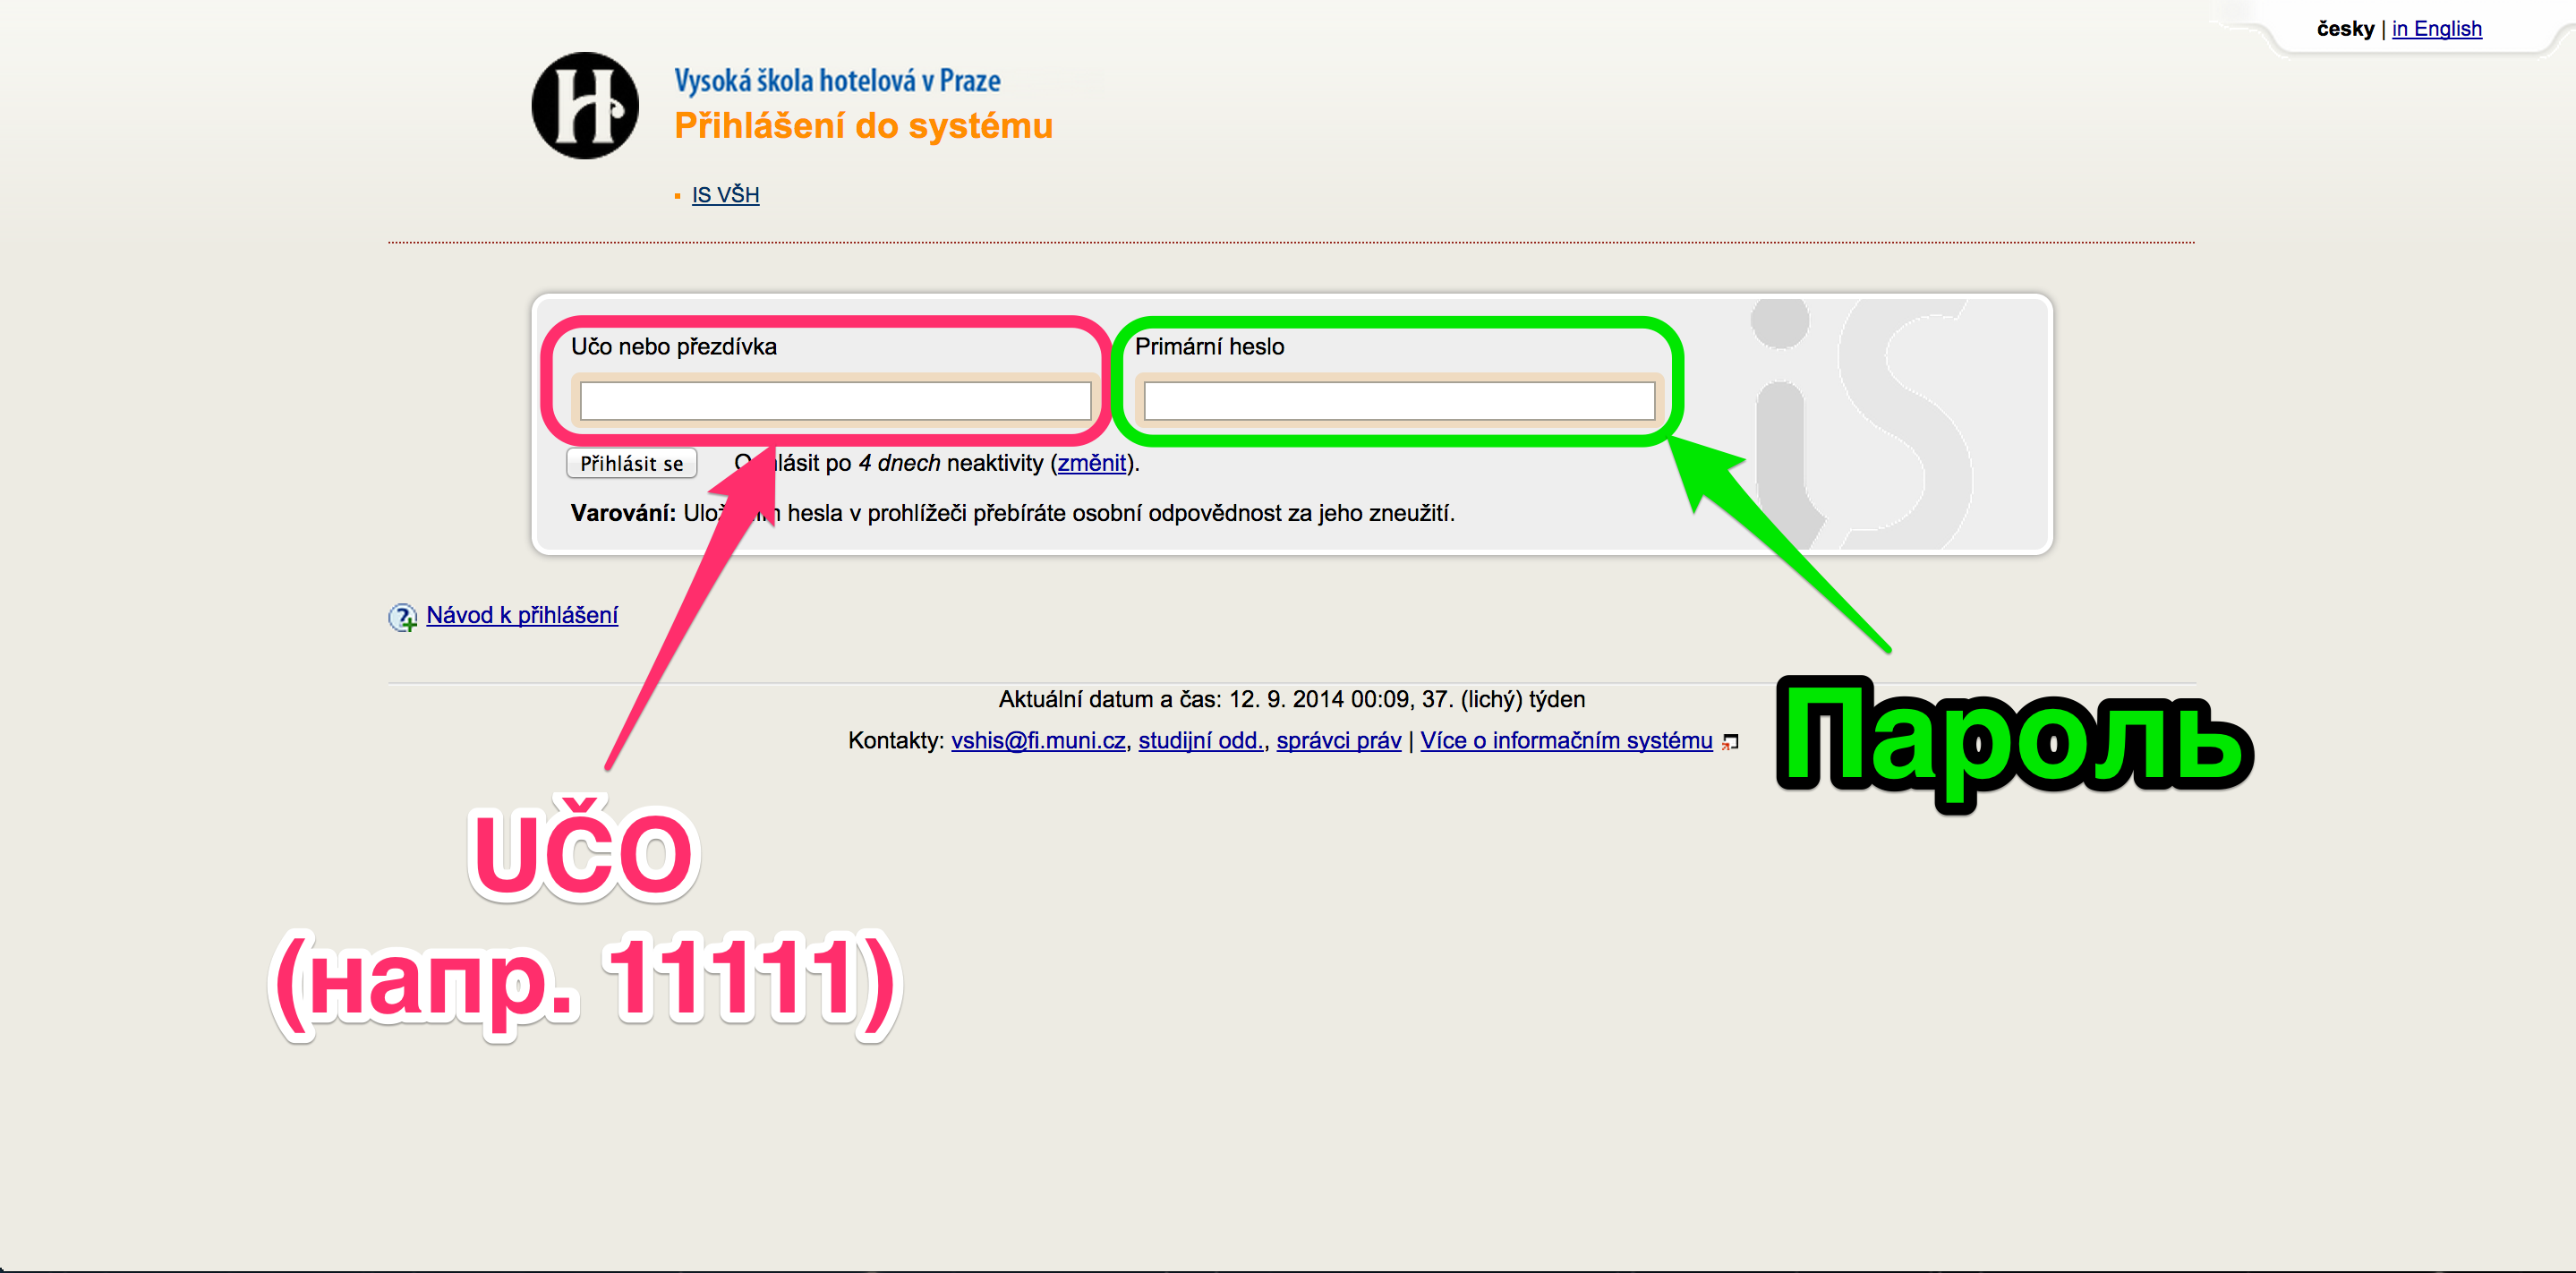
\includegraphics[width=\textwidth]{s03} \\

В левое поле \textbf{Učo nebo přezdívka} вводите свое UČO, в правое поле напишите свой пароль.
UČO и пароль у вас должны быть записаны на бумаге, которую вы получали вместе с договором об учебе.

Если все было сделано правильно, то вы попадете в систему.

\subsection{Первый взгляд}
Вот мы и на главной странице этого прекрасного творения дворников
с факультета информатики Университета Масарика. \\

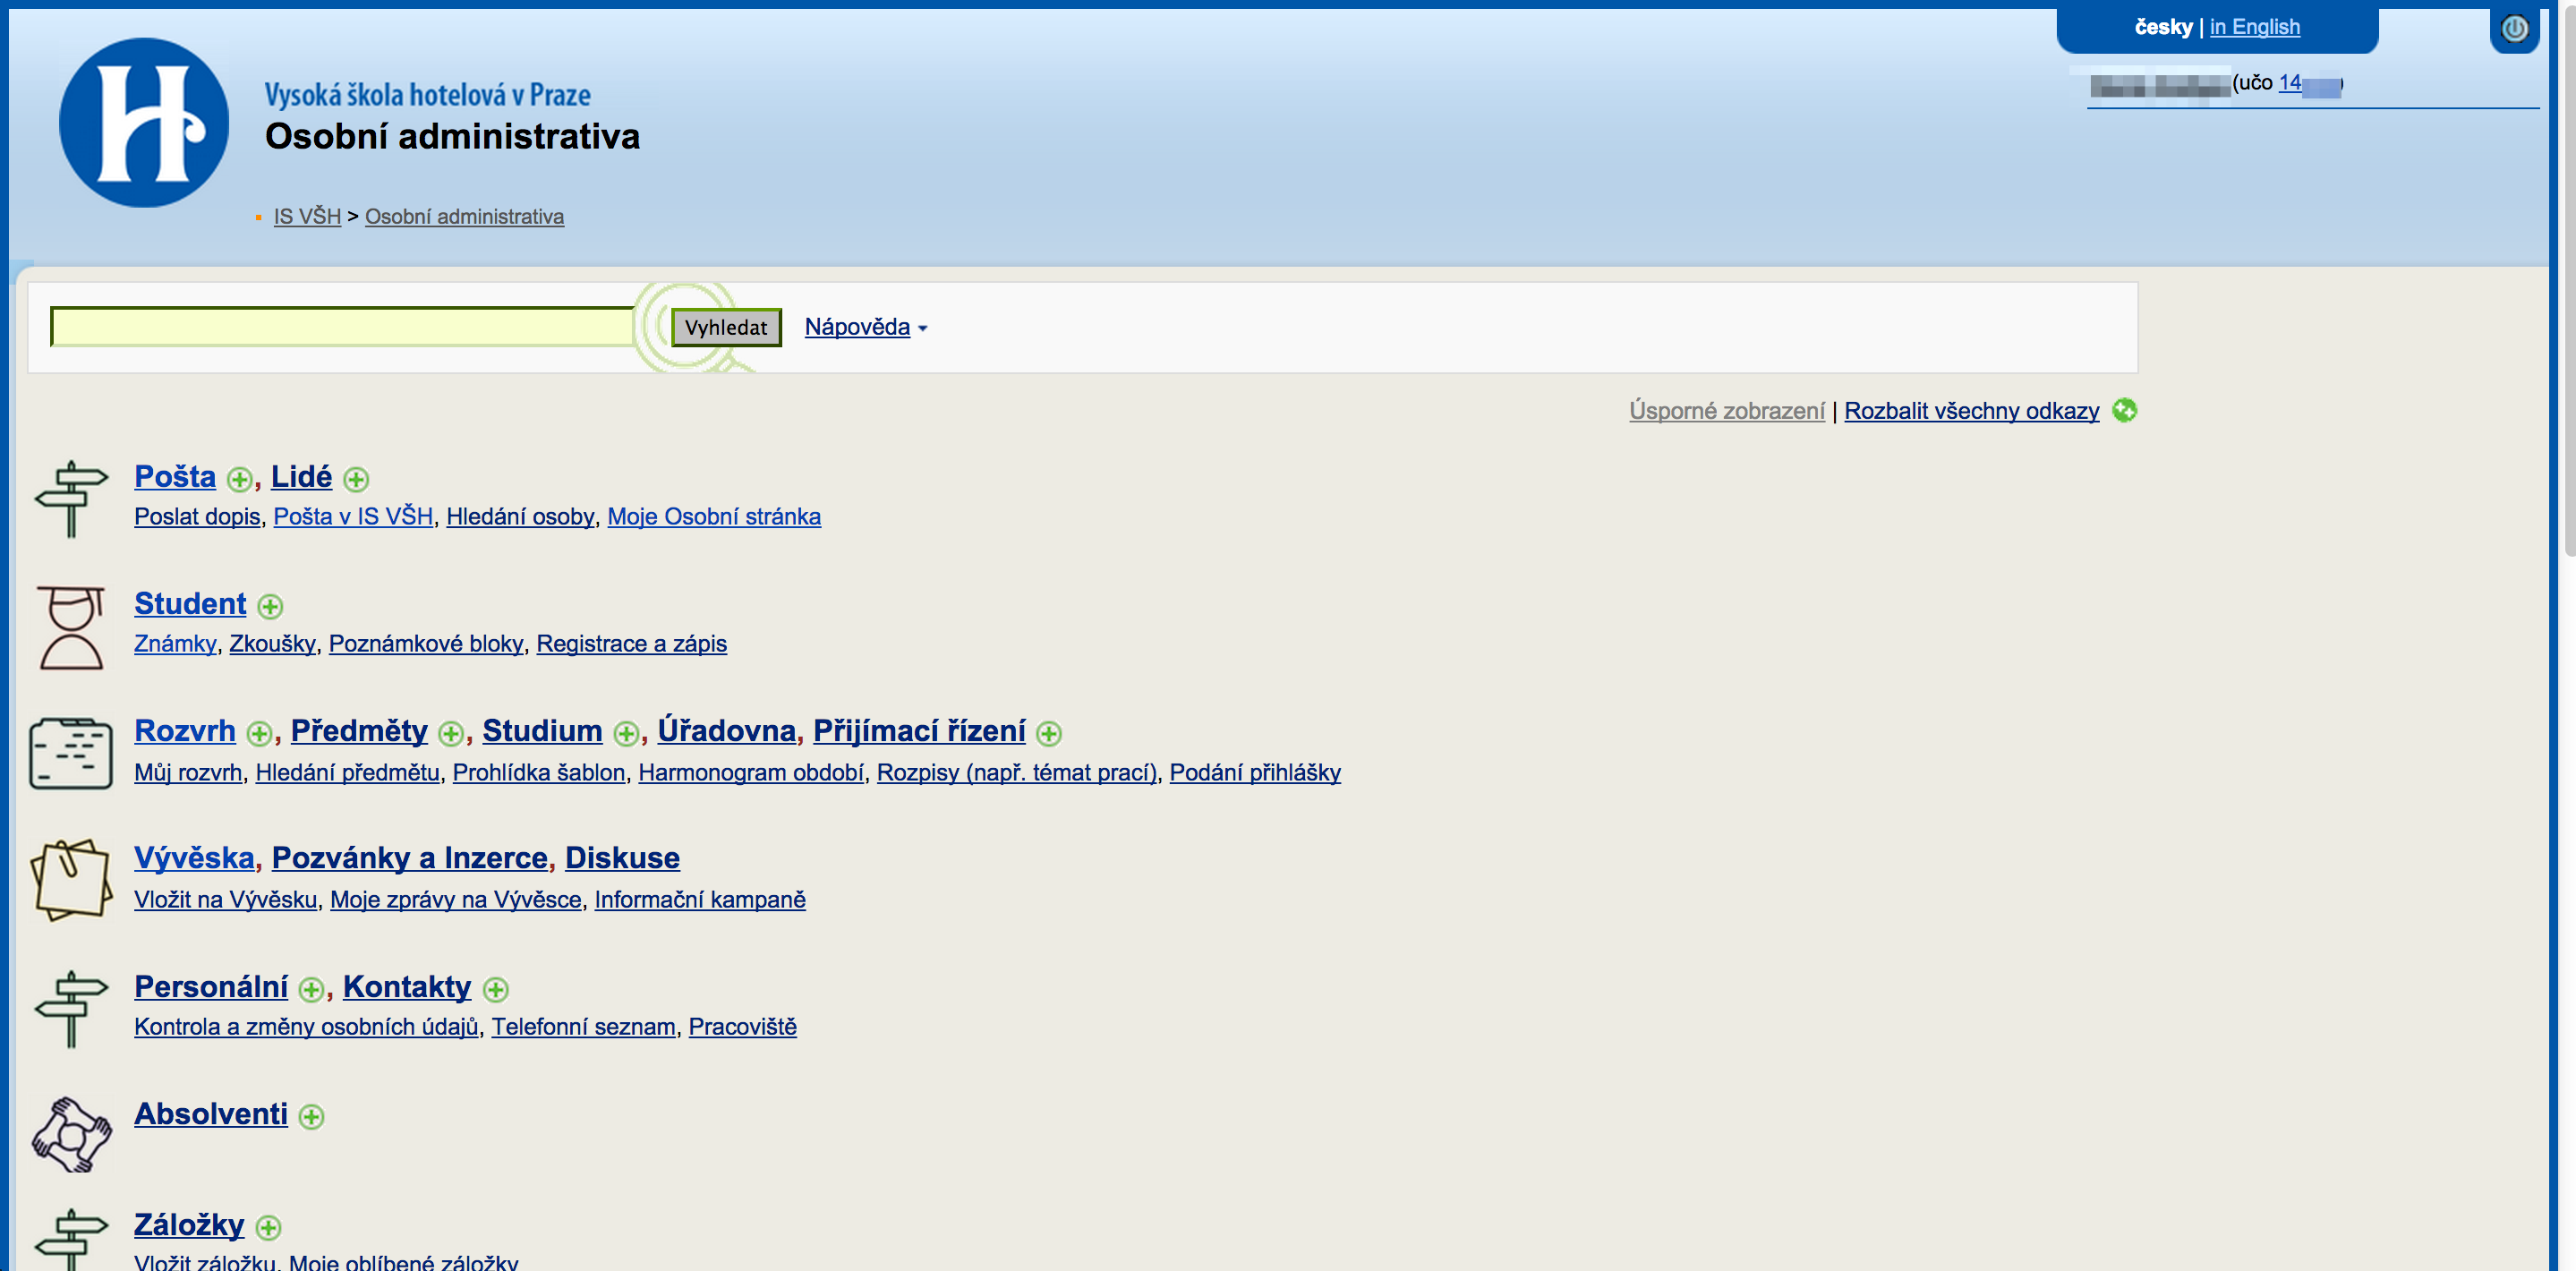
\includegraphics[width=\textwidth]{s04} \\

%Каким же Педро надо было быть, что сделать такую Кончиту?
%Еще и не побоялись написать, что это их работа. Храбрецы!
%Но перейдем к разбору интерфейса. % точнее, к его отсутствию

\newpage
\subsection{Ваш профиль}

Чтобы увидеть ваш профиль, нажмите на свой номер UČO в верхнем правом углу. \\

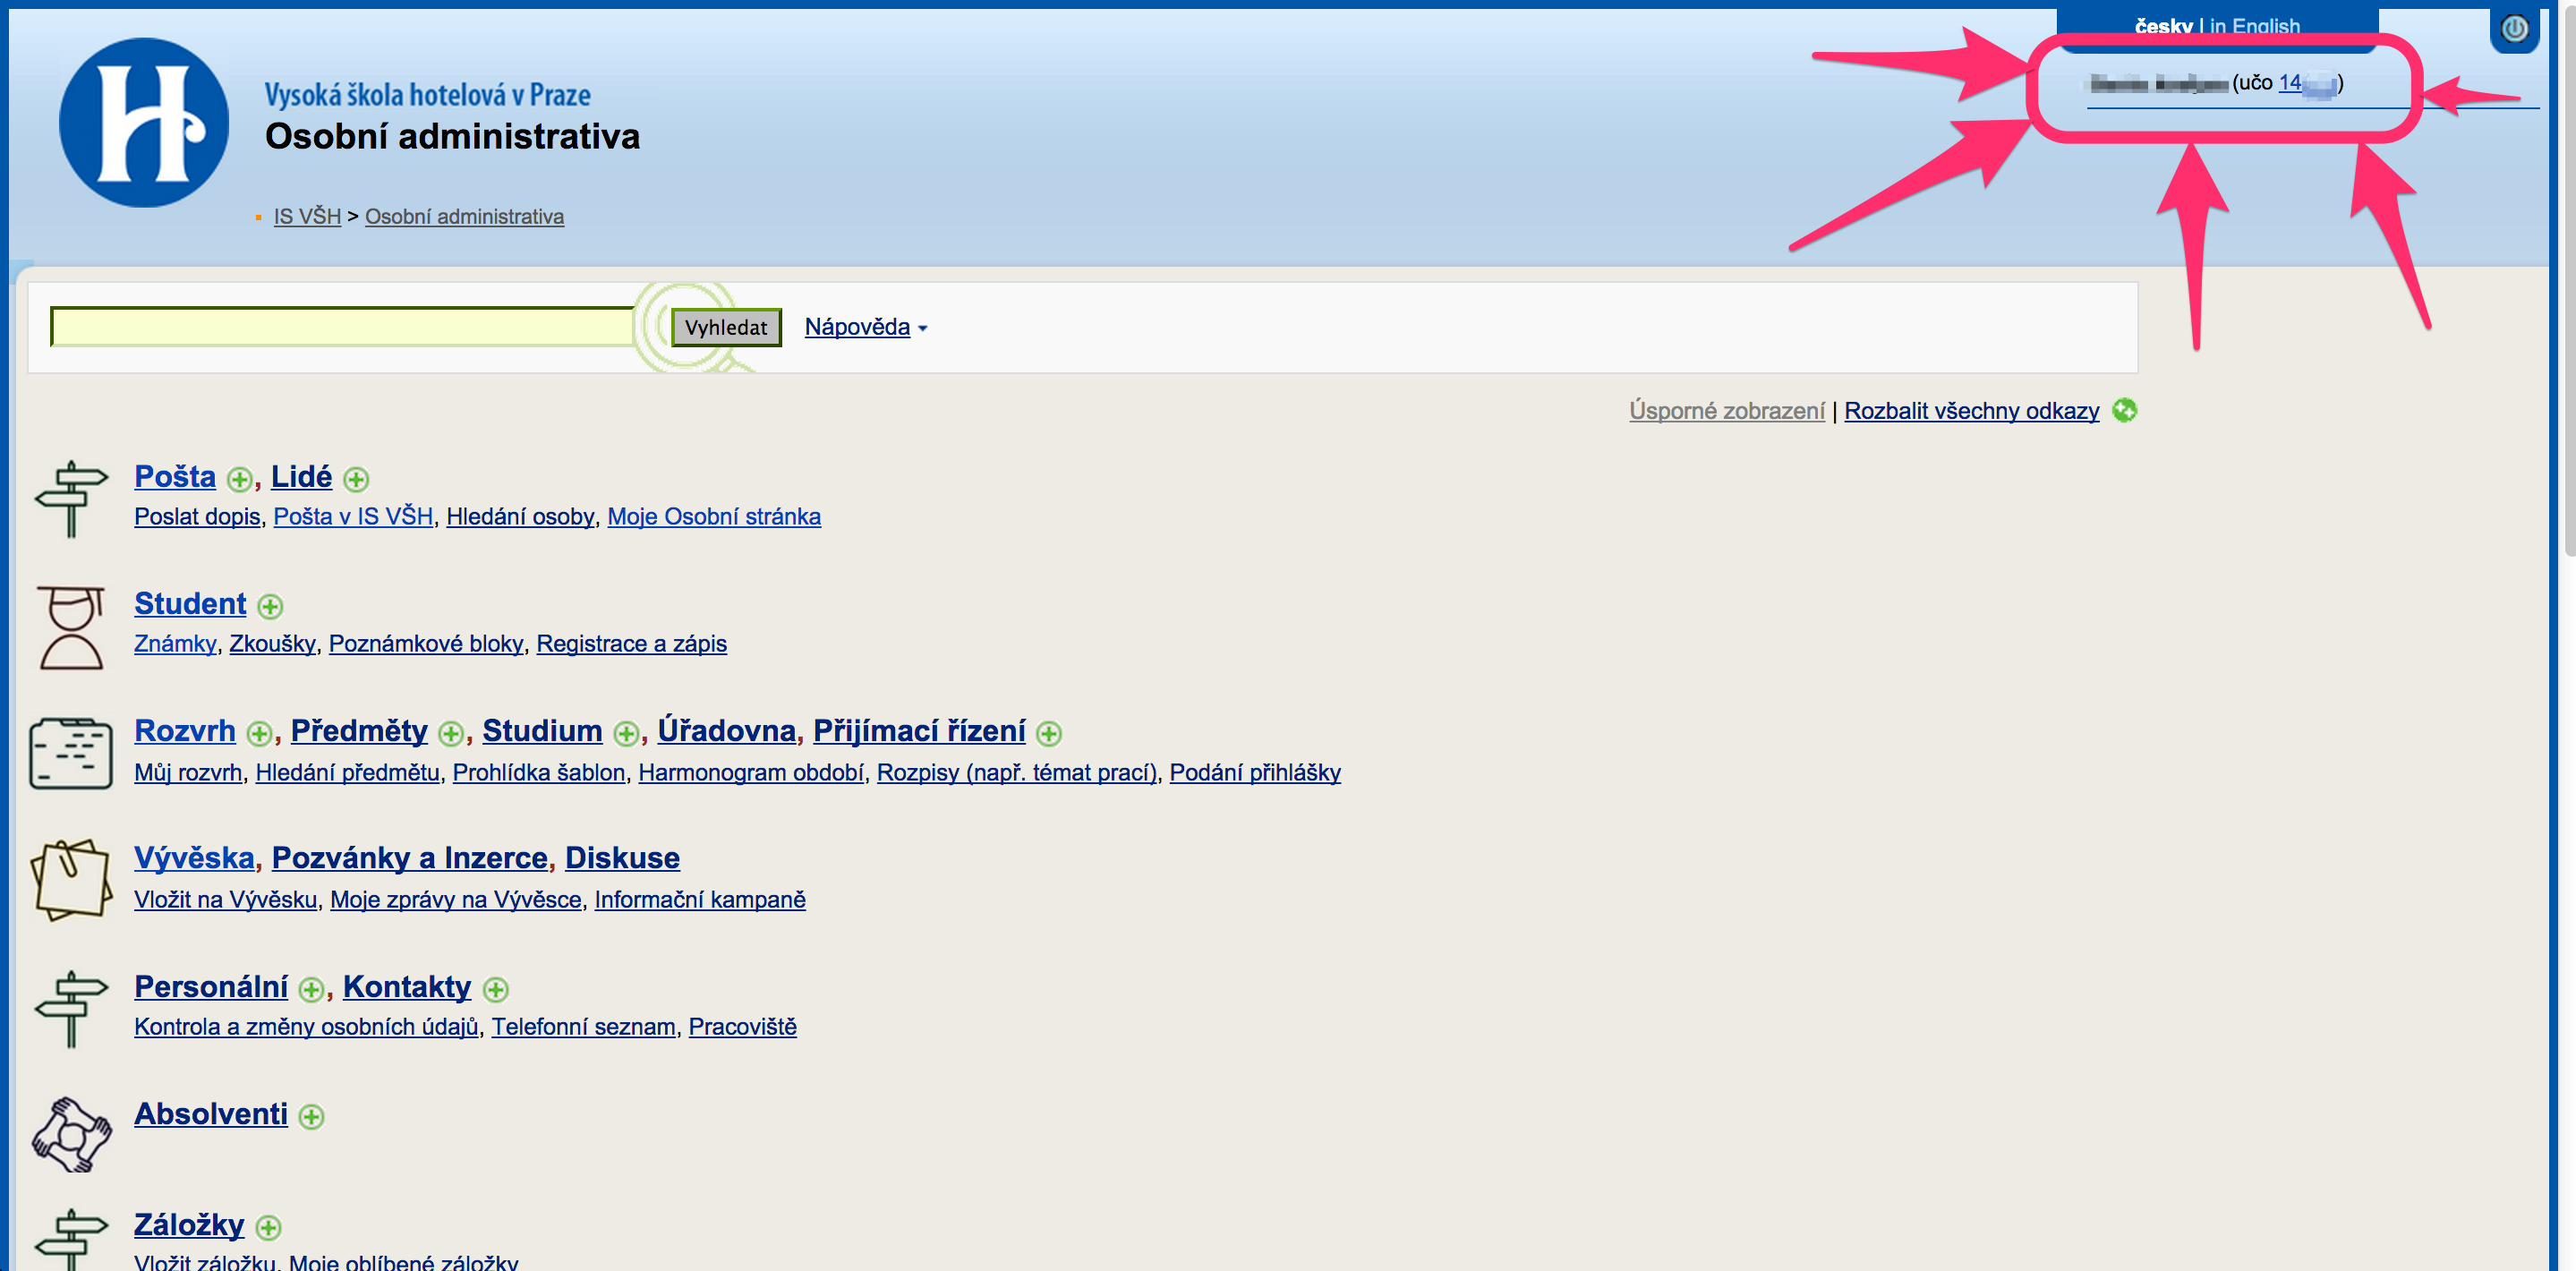
\includegraphics[width=\textwidth]{s05} \\

В разделе своего профиля вы найдете свою фотографию, свои имя и UČO, 
факультет, специальность и группу. \\

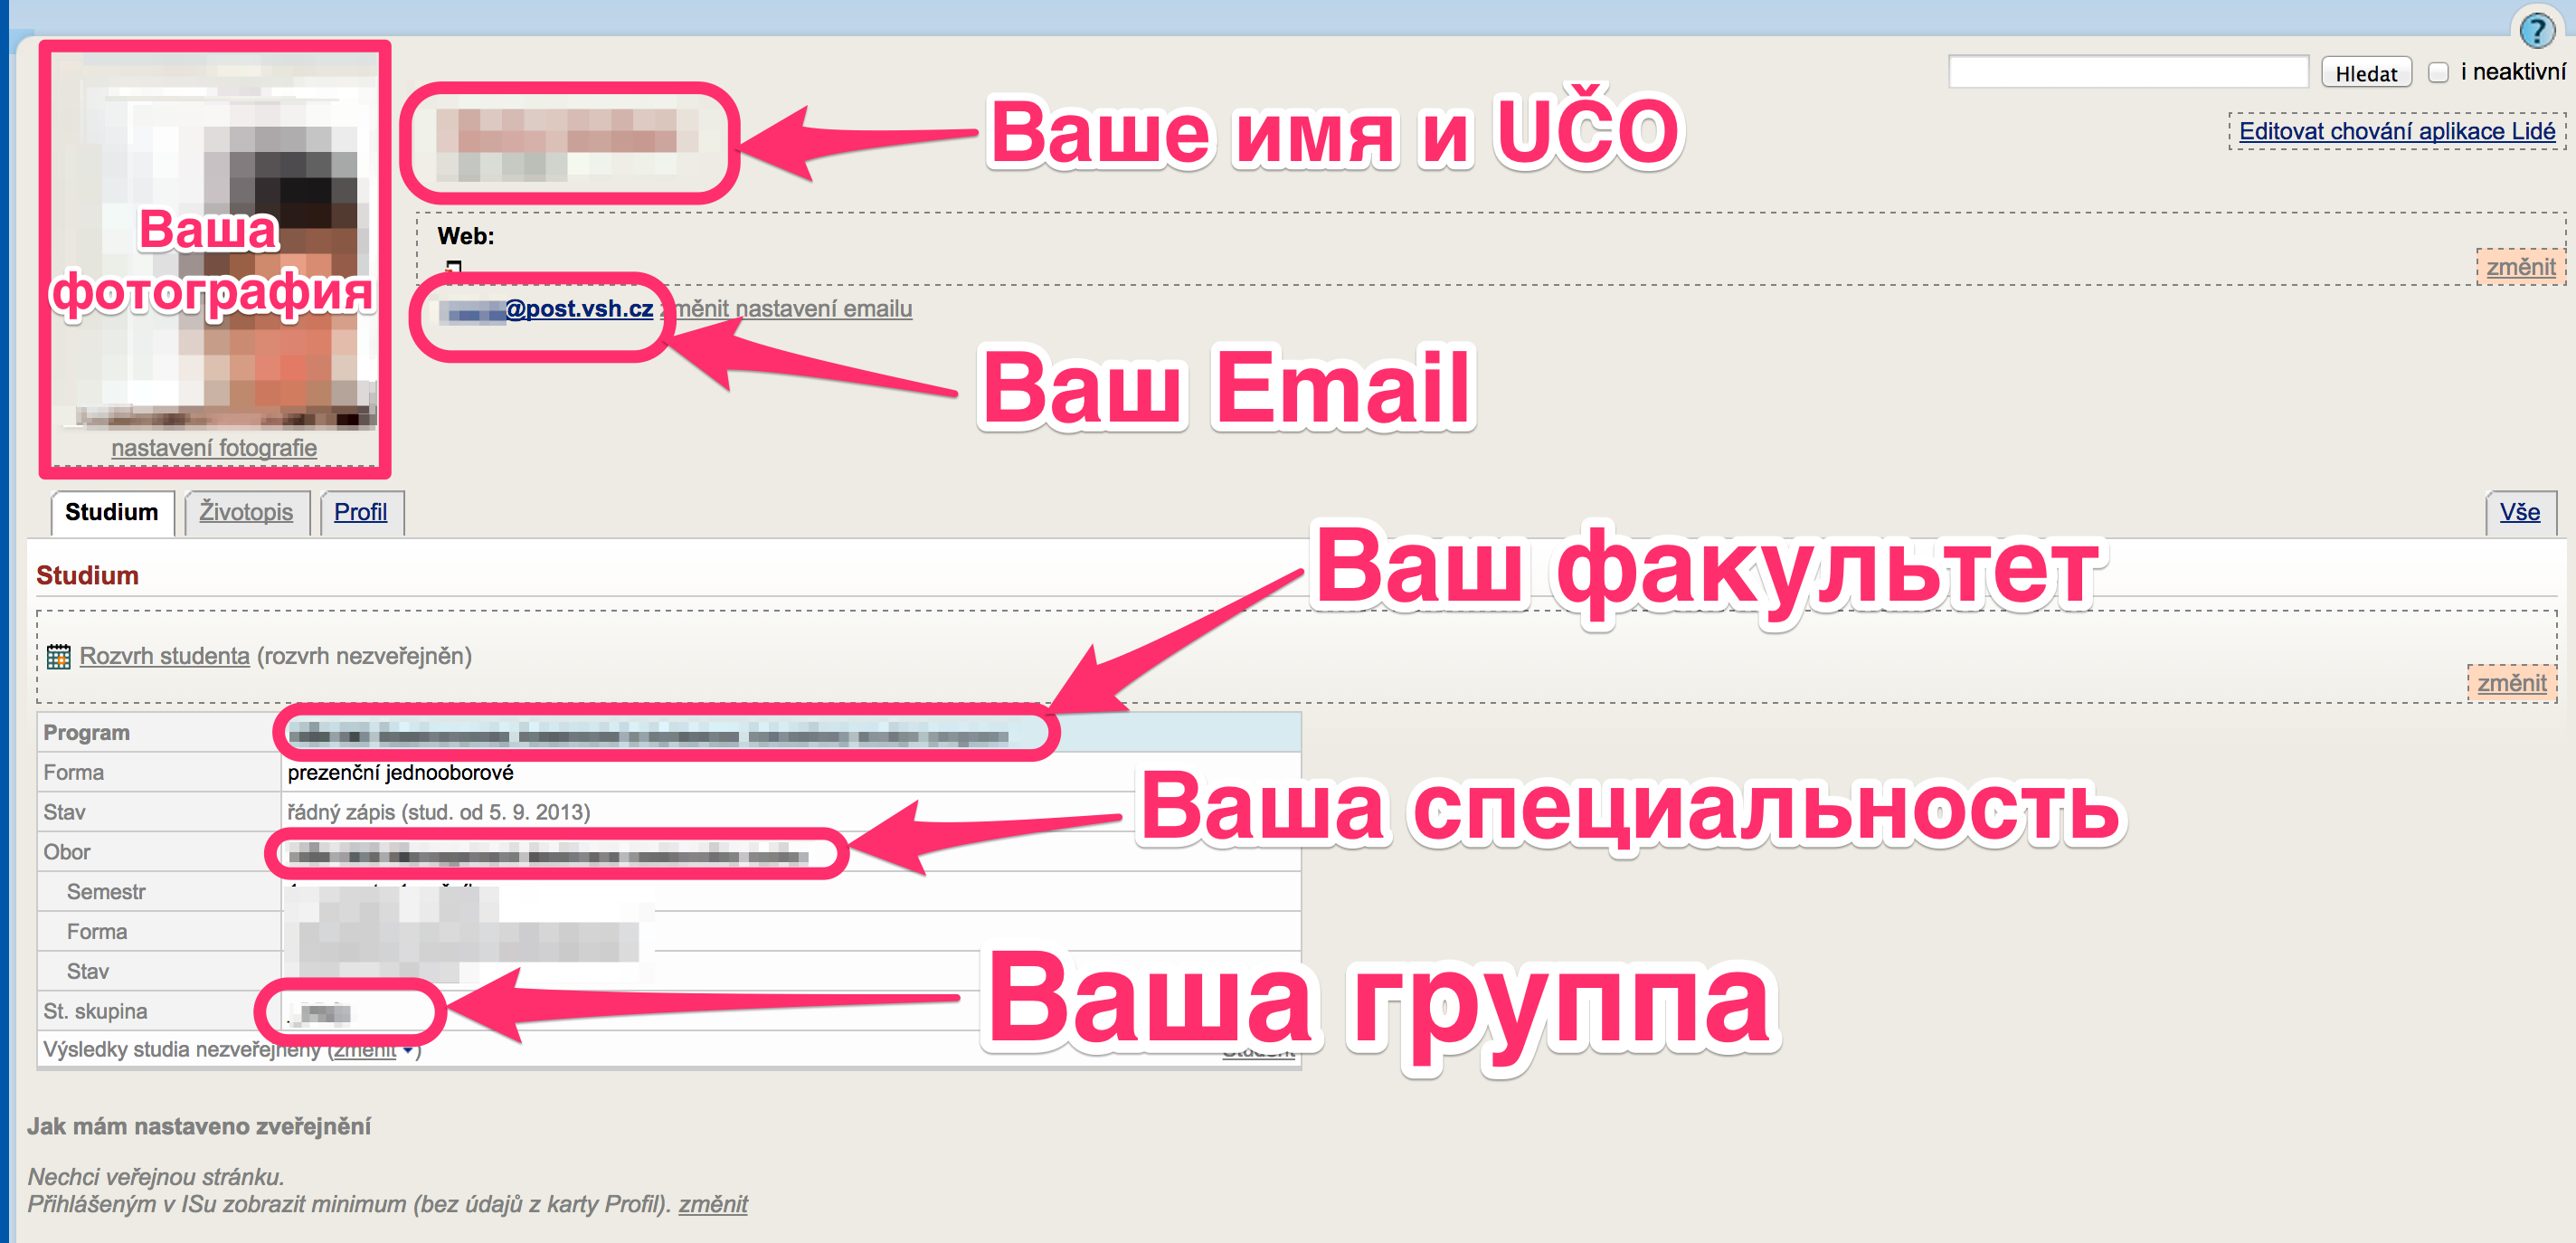
\includegraphics[width=\textwidth]{s06} \\

\newpage
Чтобы вернуться в главное меню, просто нажмите на лого школы, 
или нажмите на ссылку \textbf{IS VŠH} под ним. \\

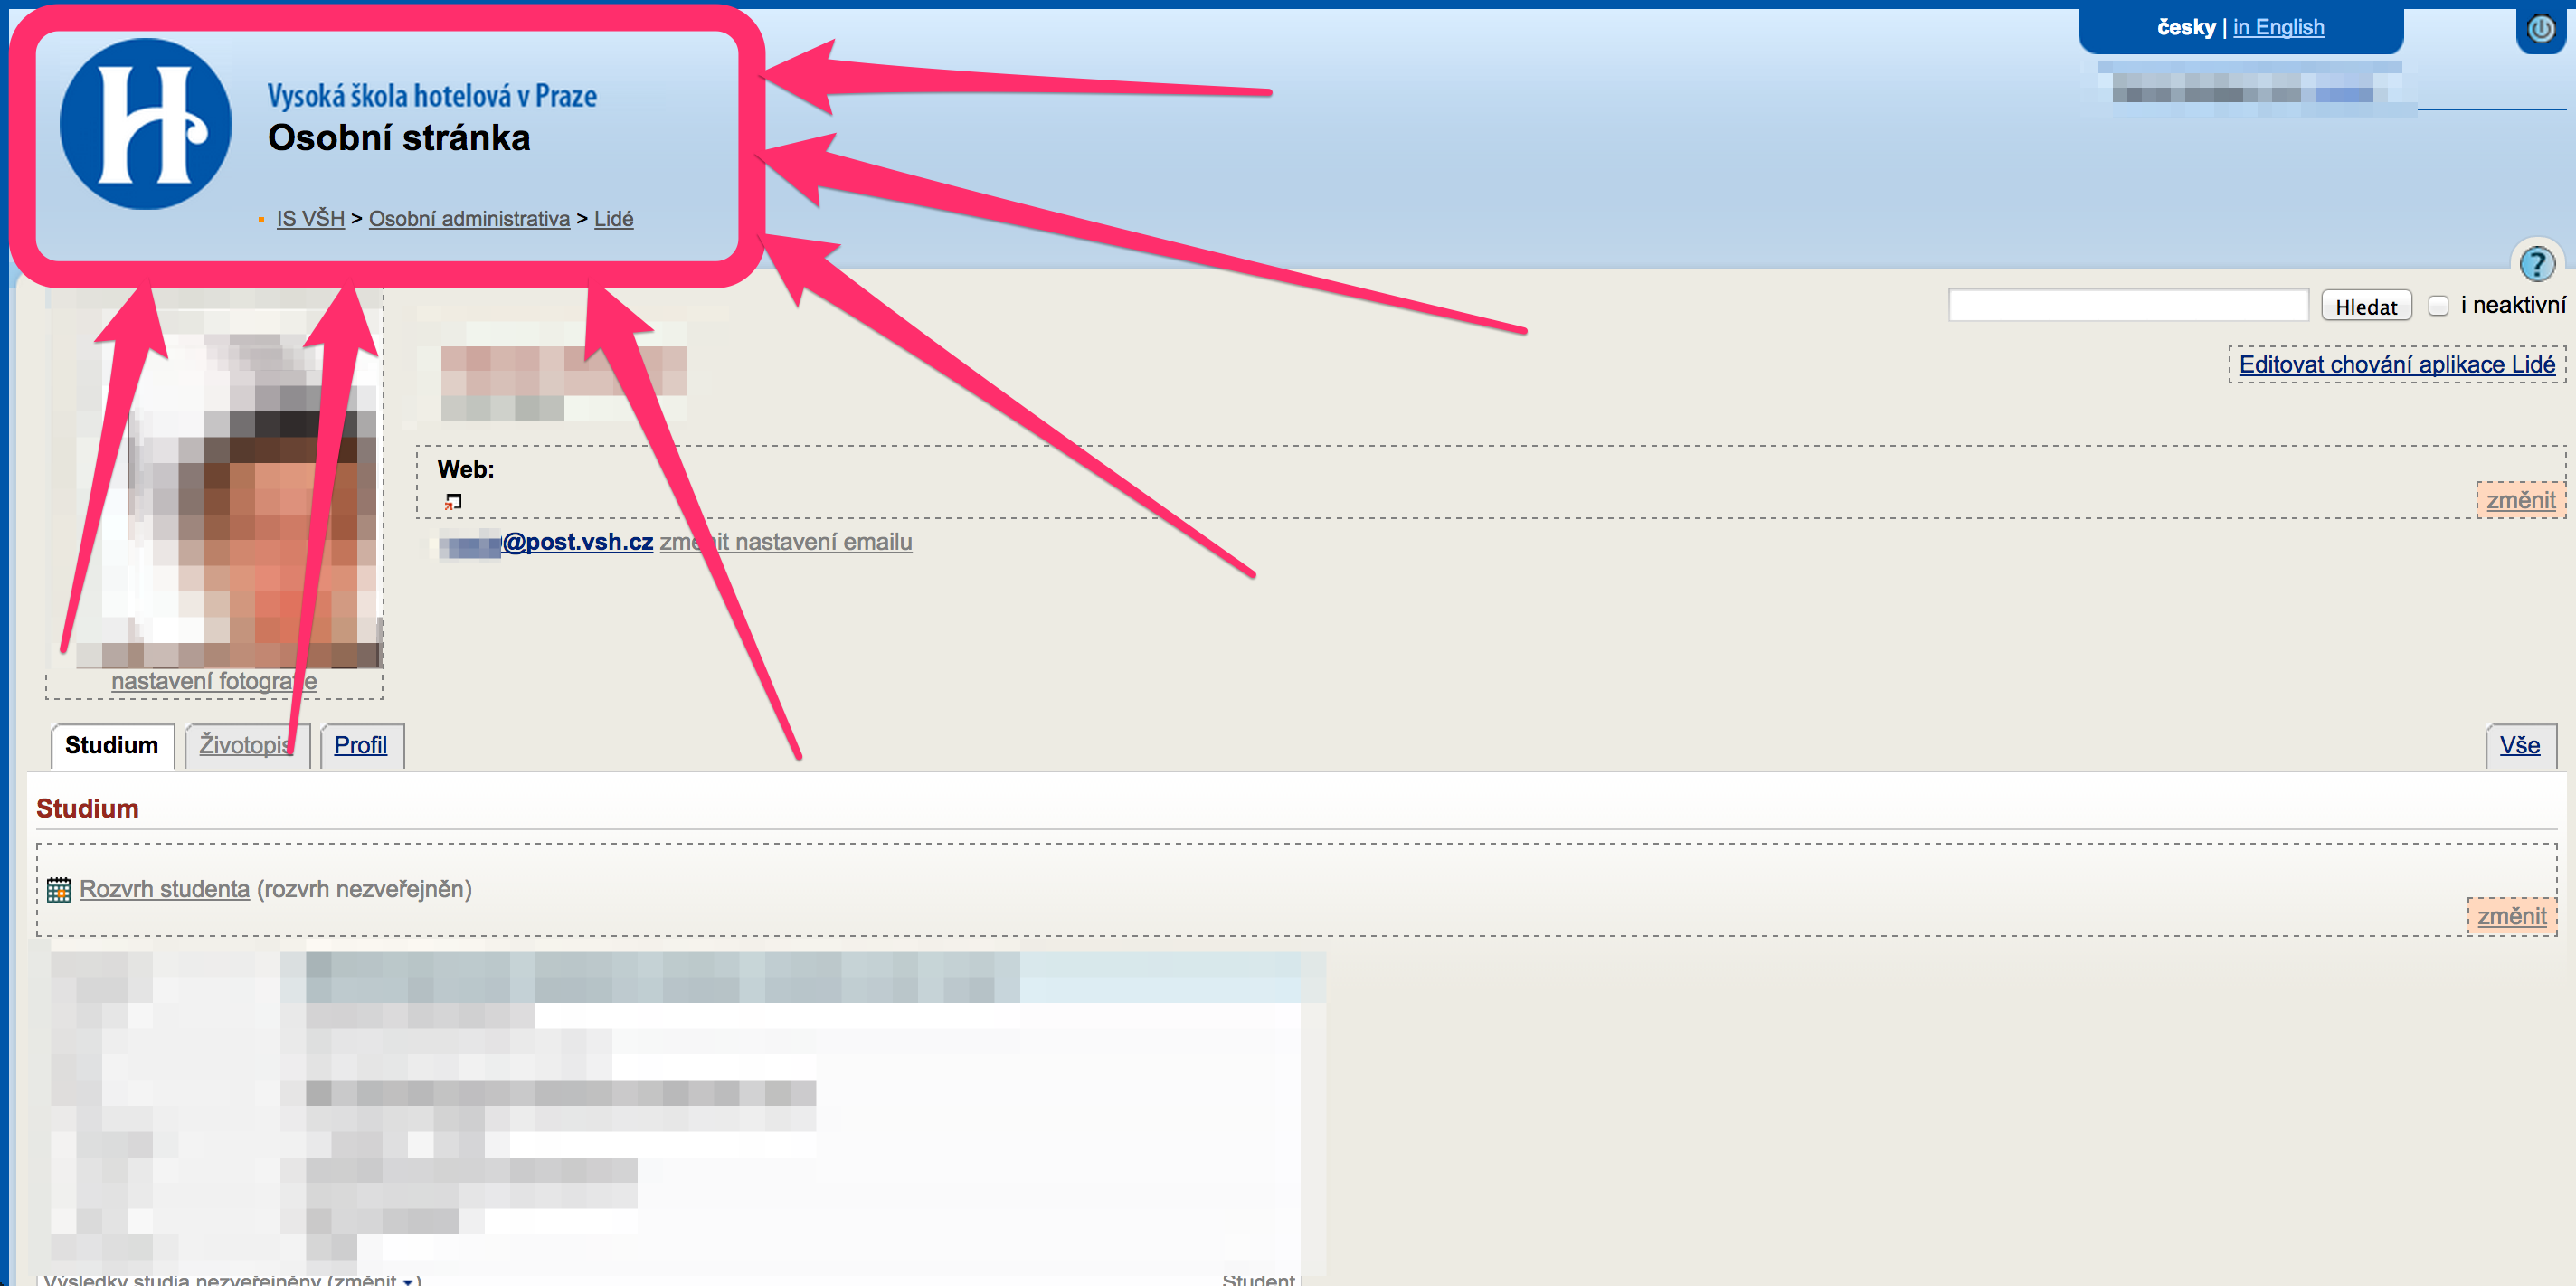
\includegraphics[width=\textwidth]{s07} \\

Вуаля! Мы снова на главной странице! \\

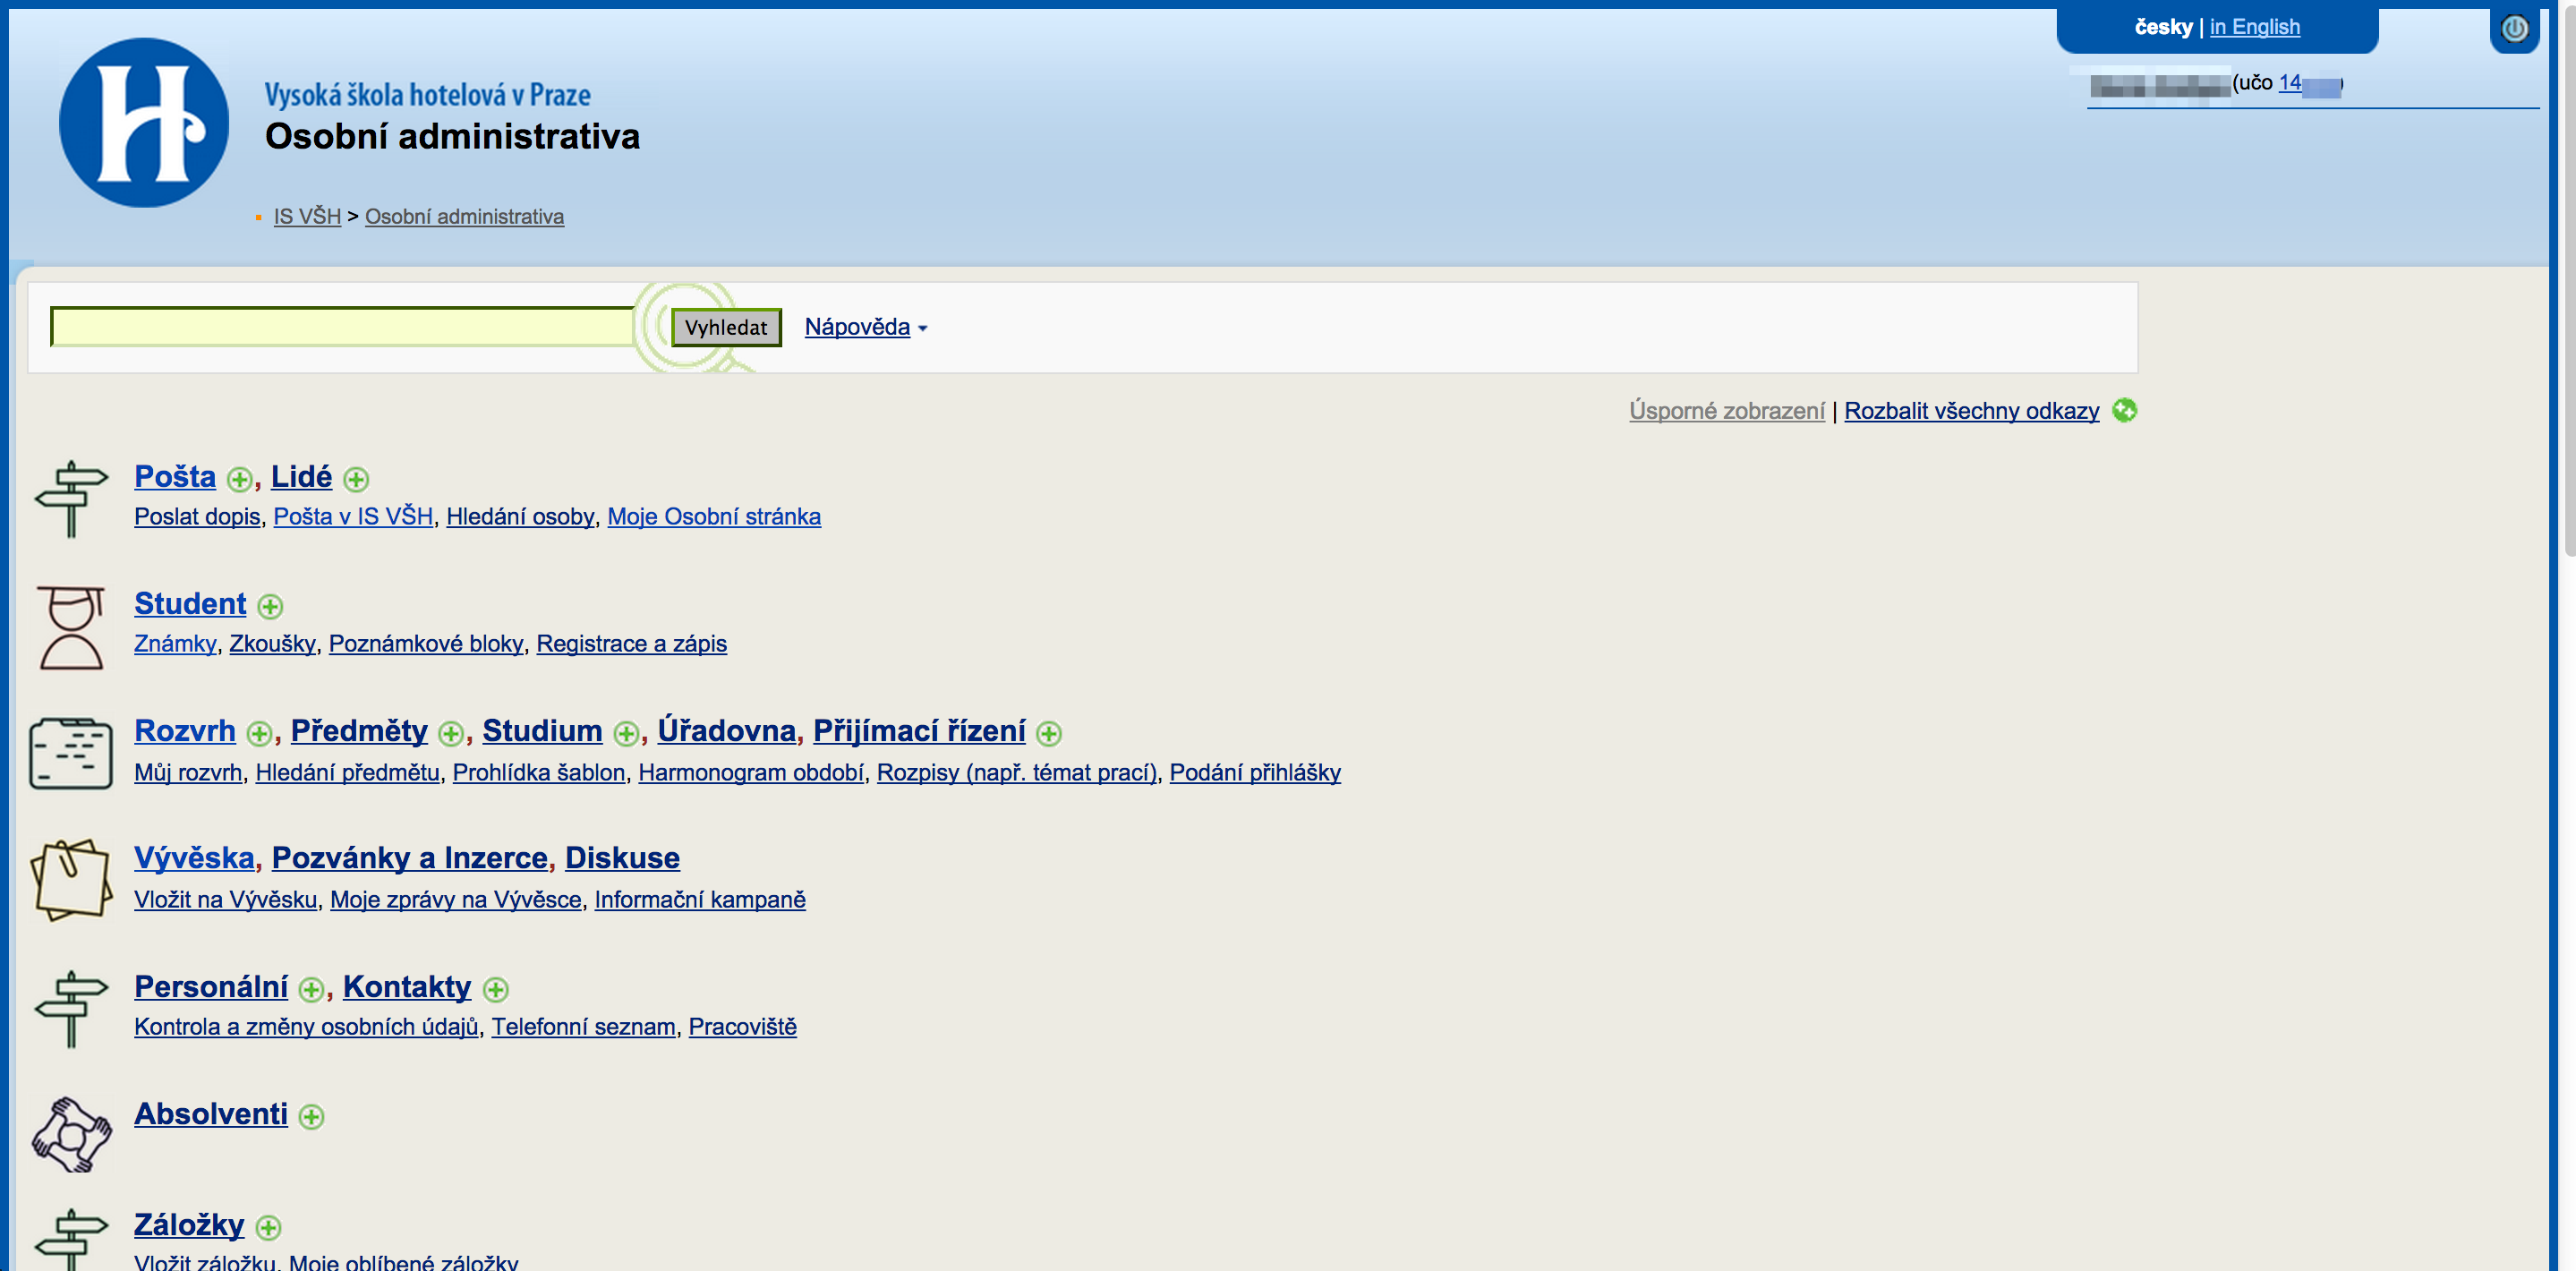
\includegraphics[width=\textwidth]{s04} \\

\newpage

\section{Ваша почта}
Так выглядит почта. Сюда будет приходить вся важная информация, касающаяся вашего обучения.
Советую проверять почаще, чтобы ничего не пропустить. \\

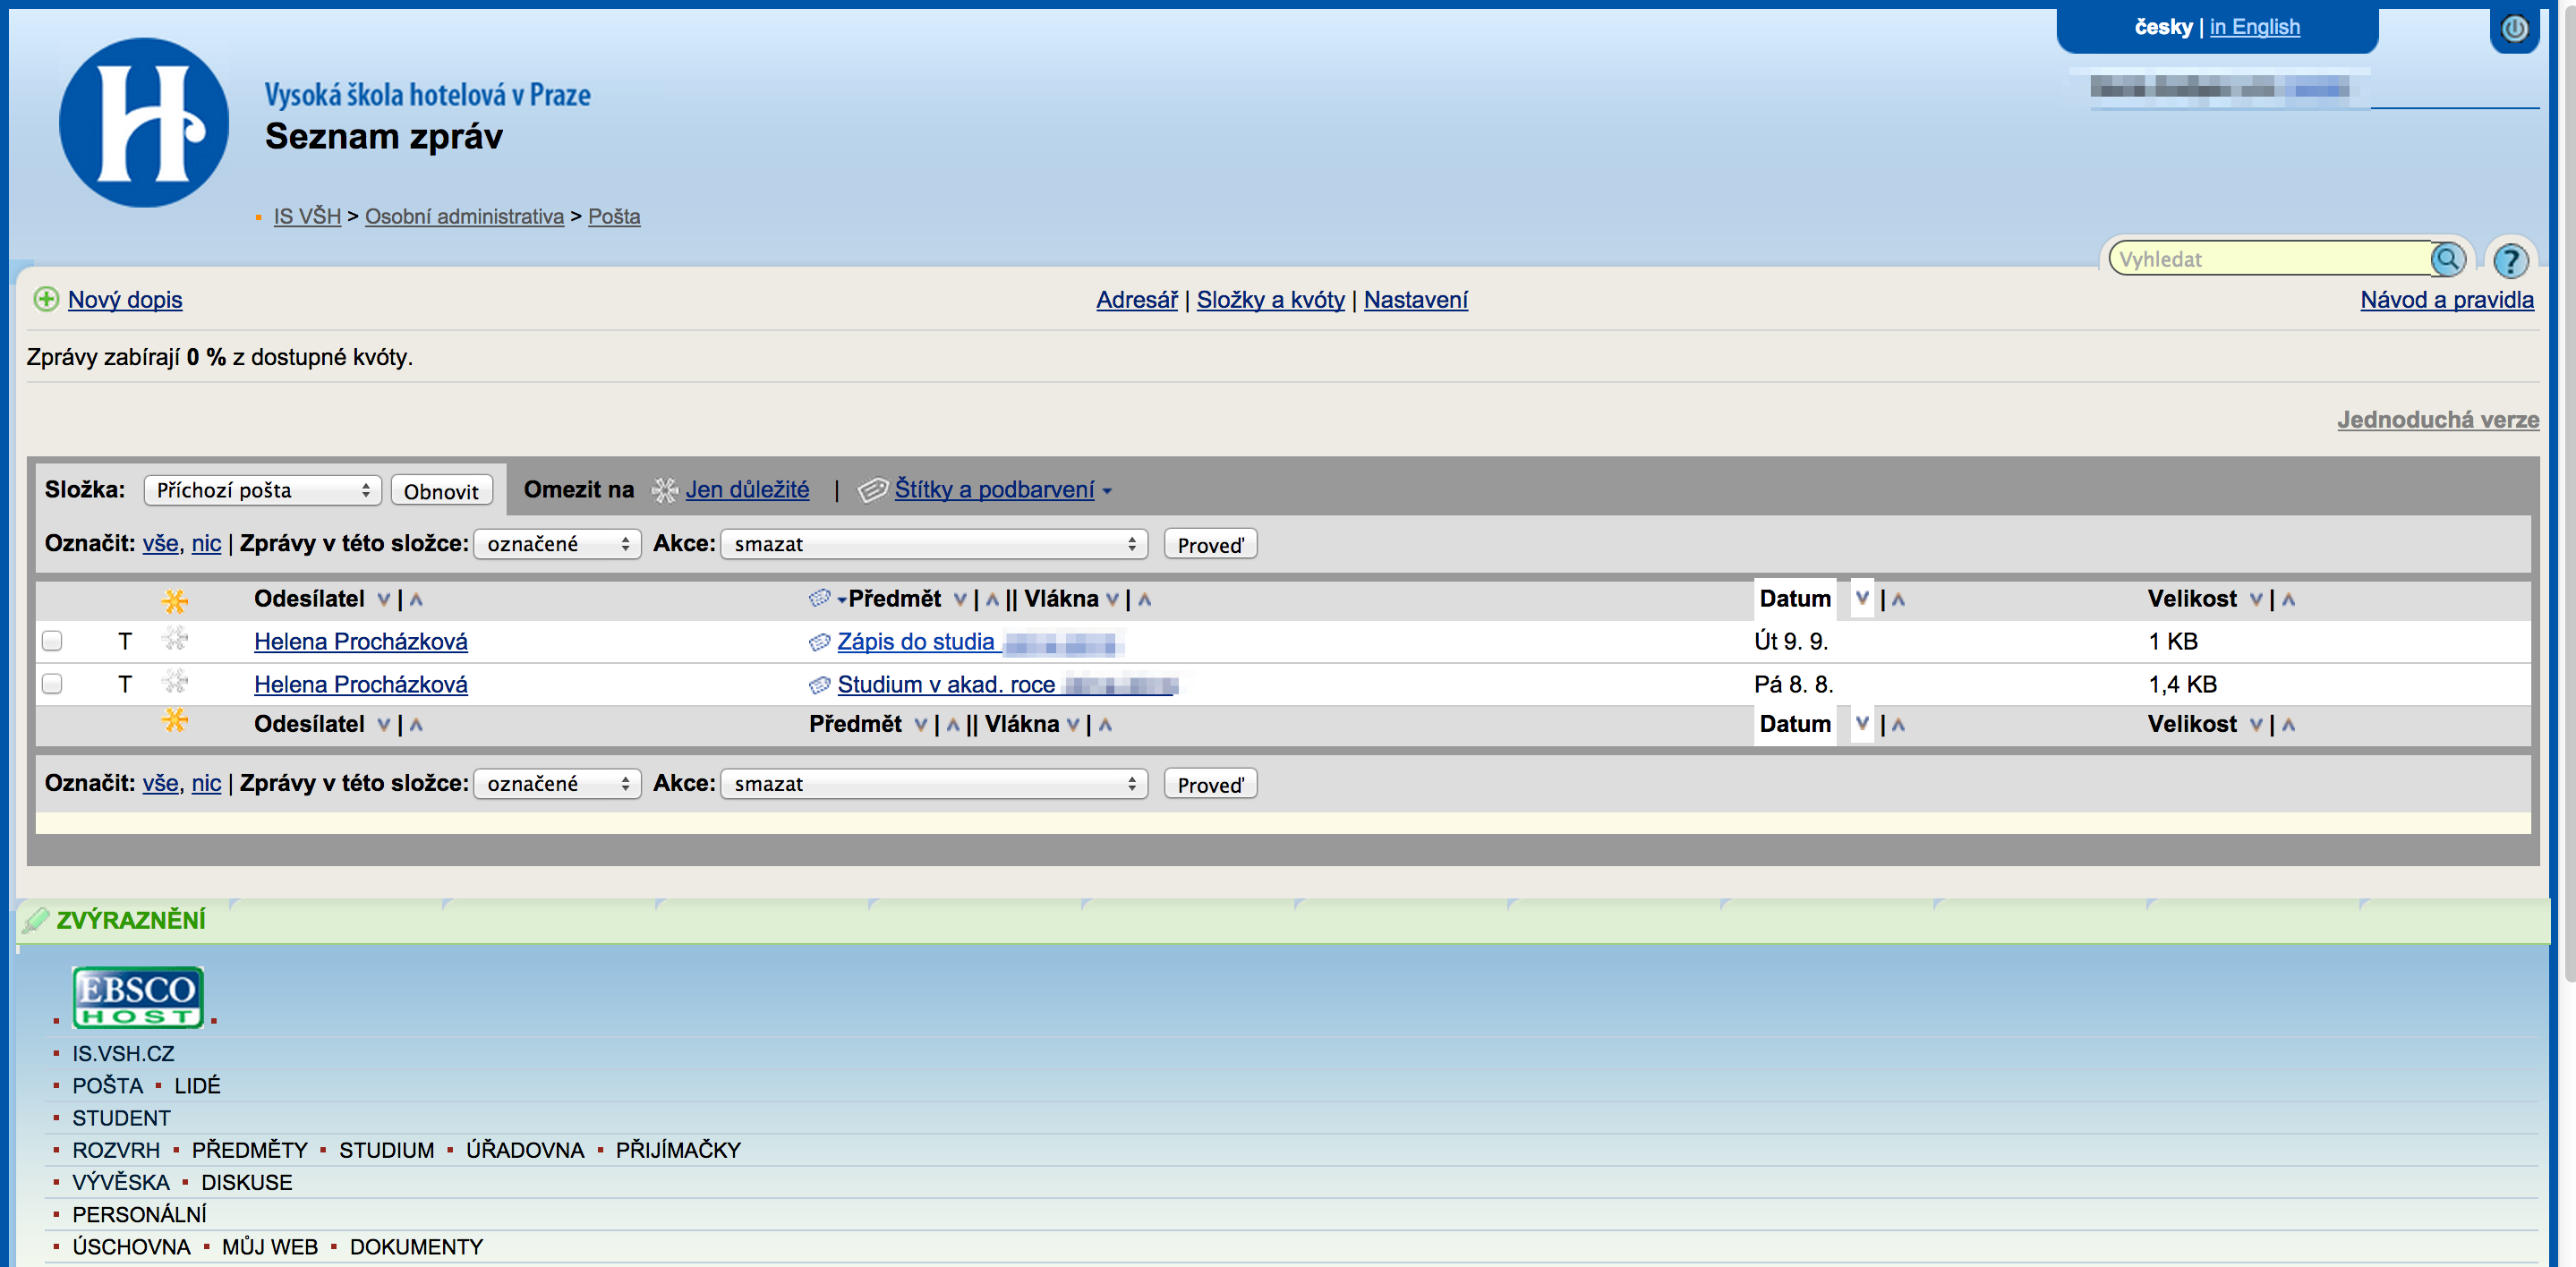
\includegraphics[width=\textwidth]{s08}

\subsection{Написать письмо}

Чтобы написать новое письмо, просто нажмите на ссылку \textbf{Nový dopis} вверху слева. \\

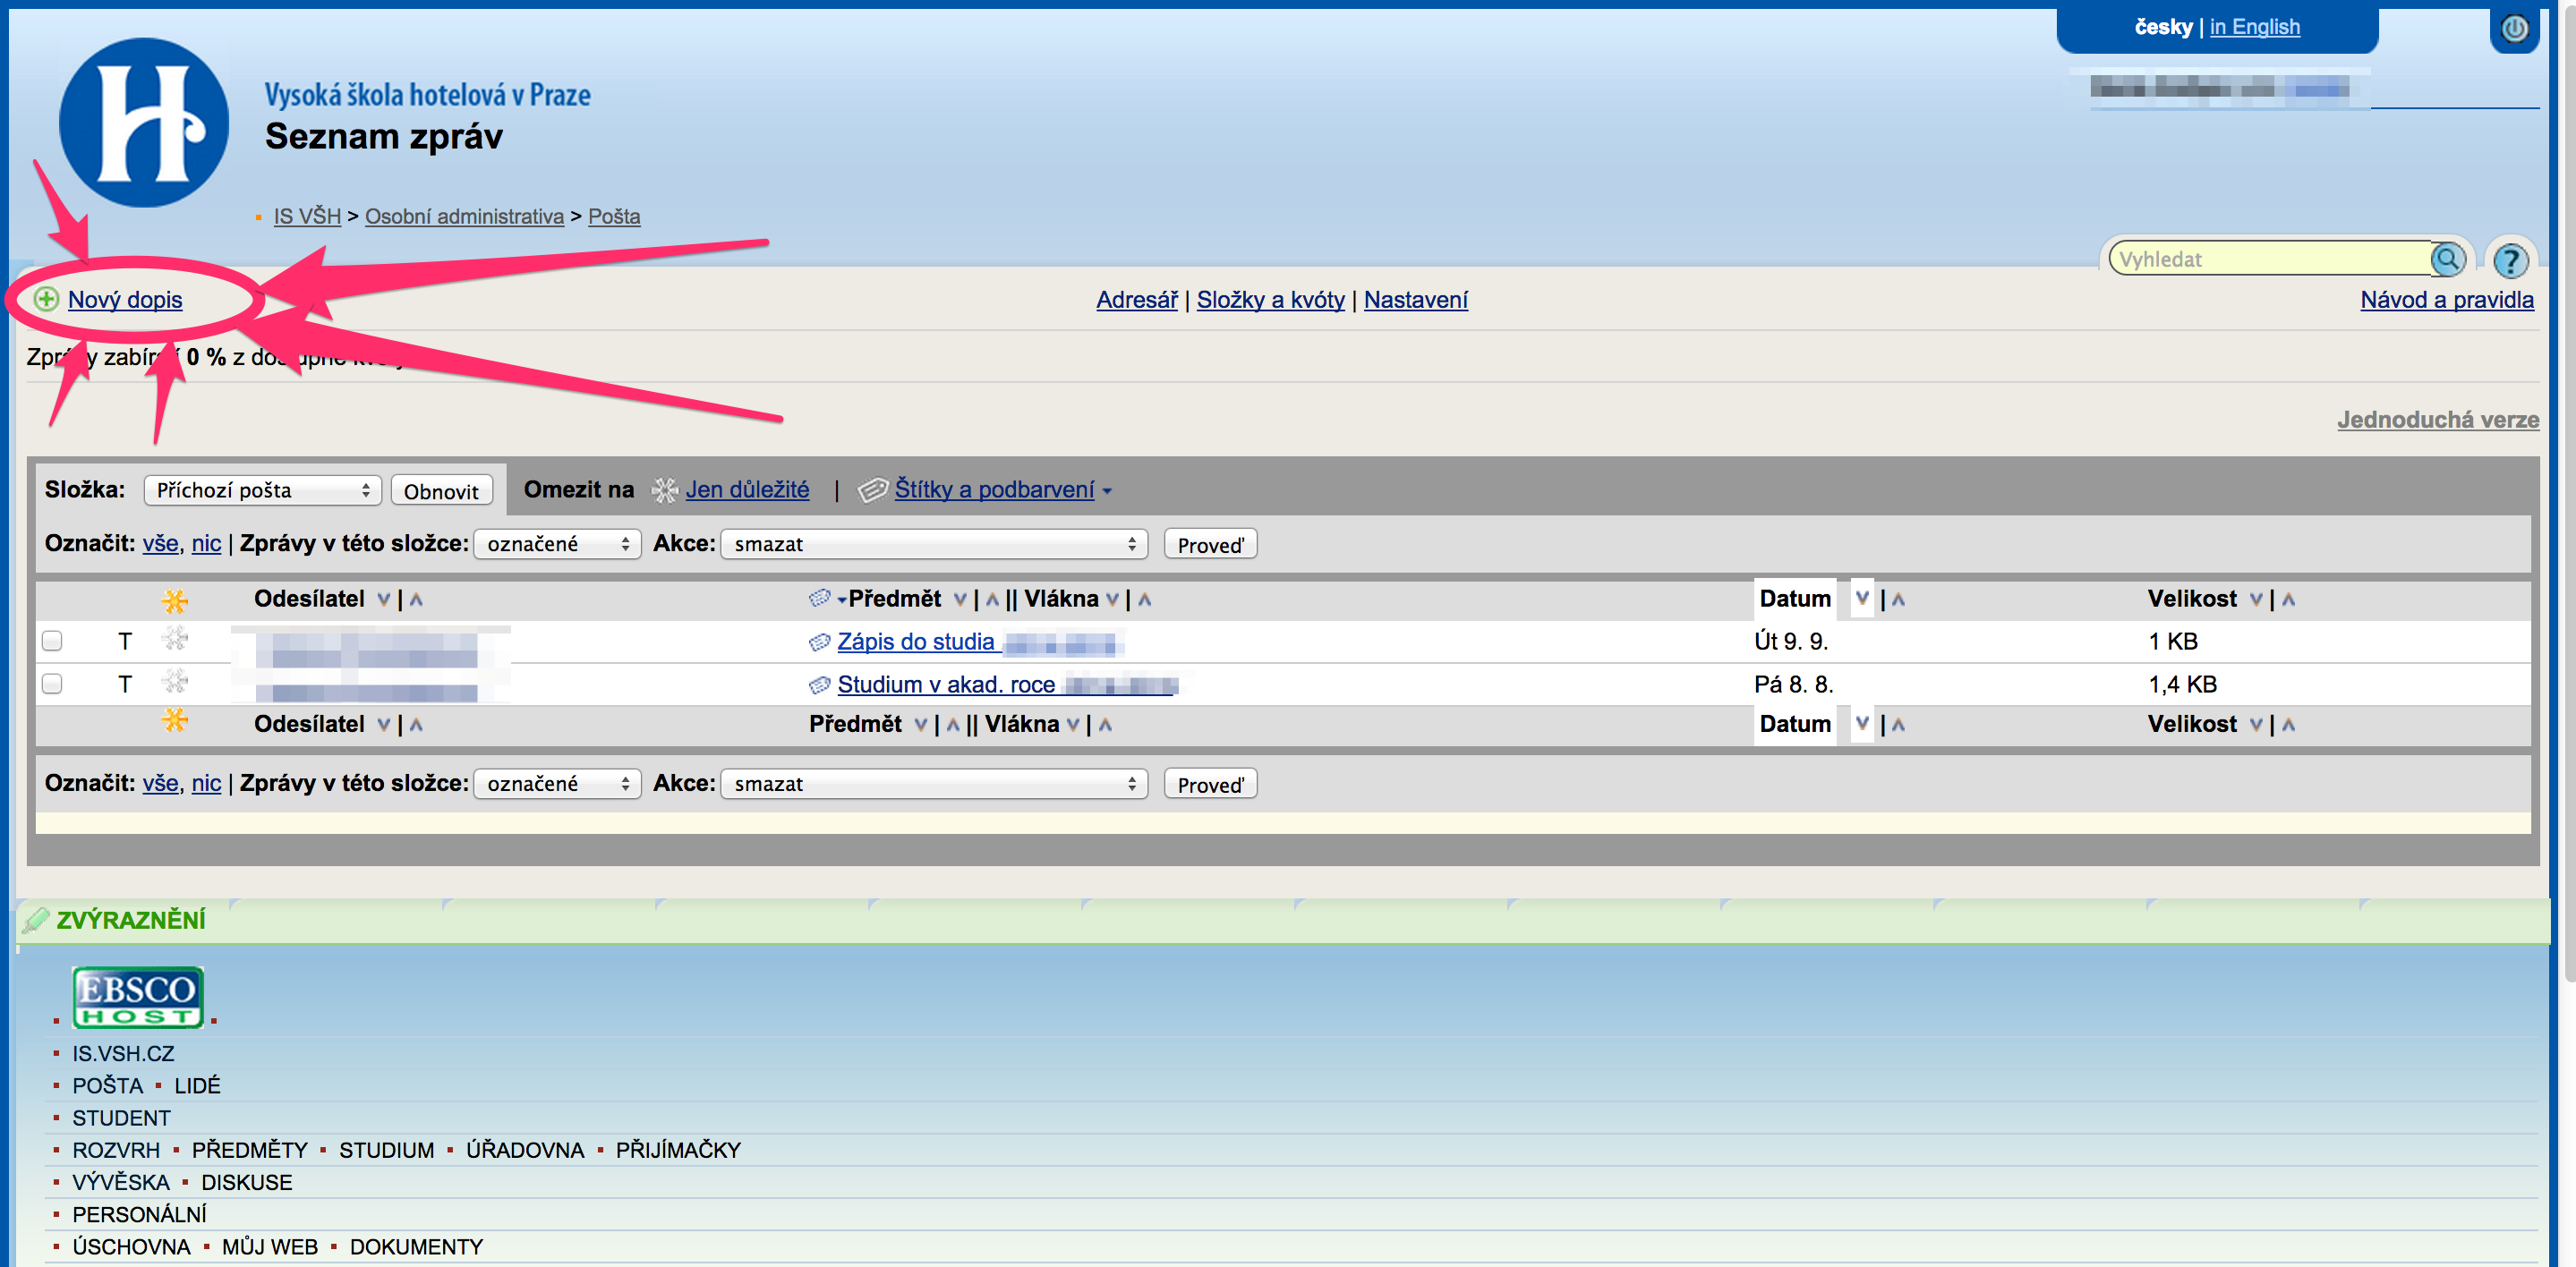
\includegraphics[width=\textwidth]{s09}

\newpage
Вы попадете на новую страницу, где вы сможете написать письмо любому нужному 
(или не очень нужному, любимому... нужное подчеркнуть) человеку. \\

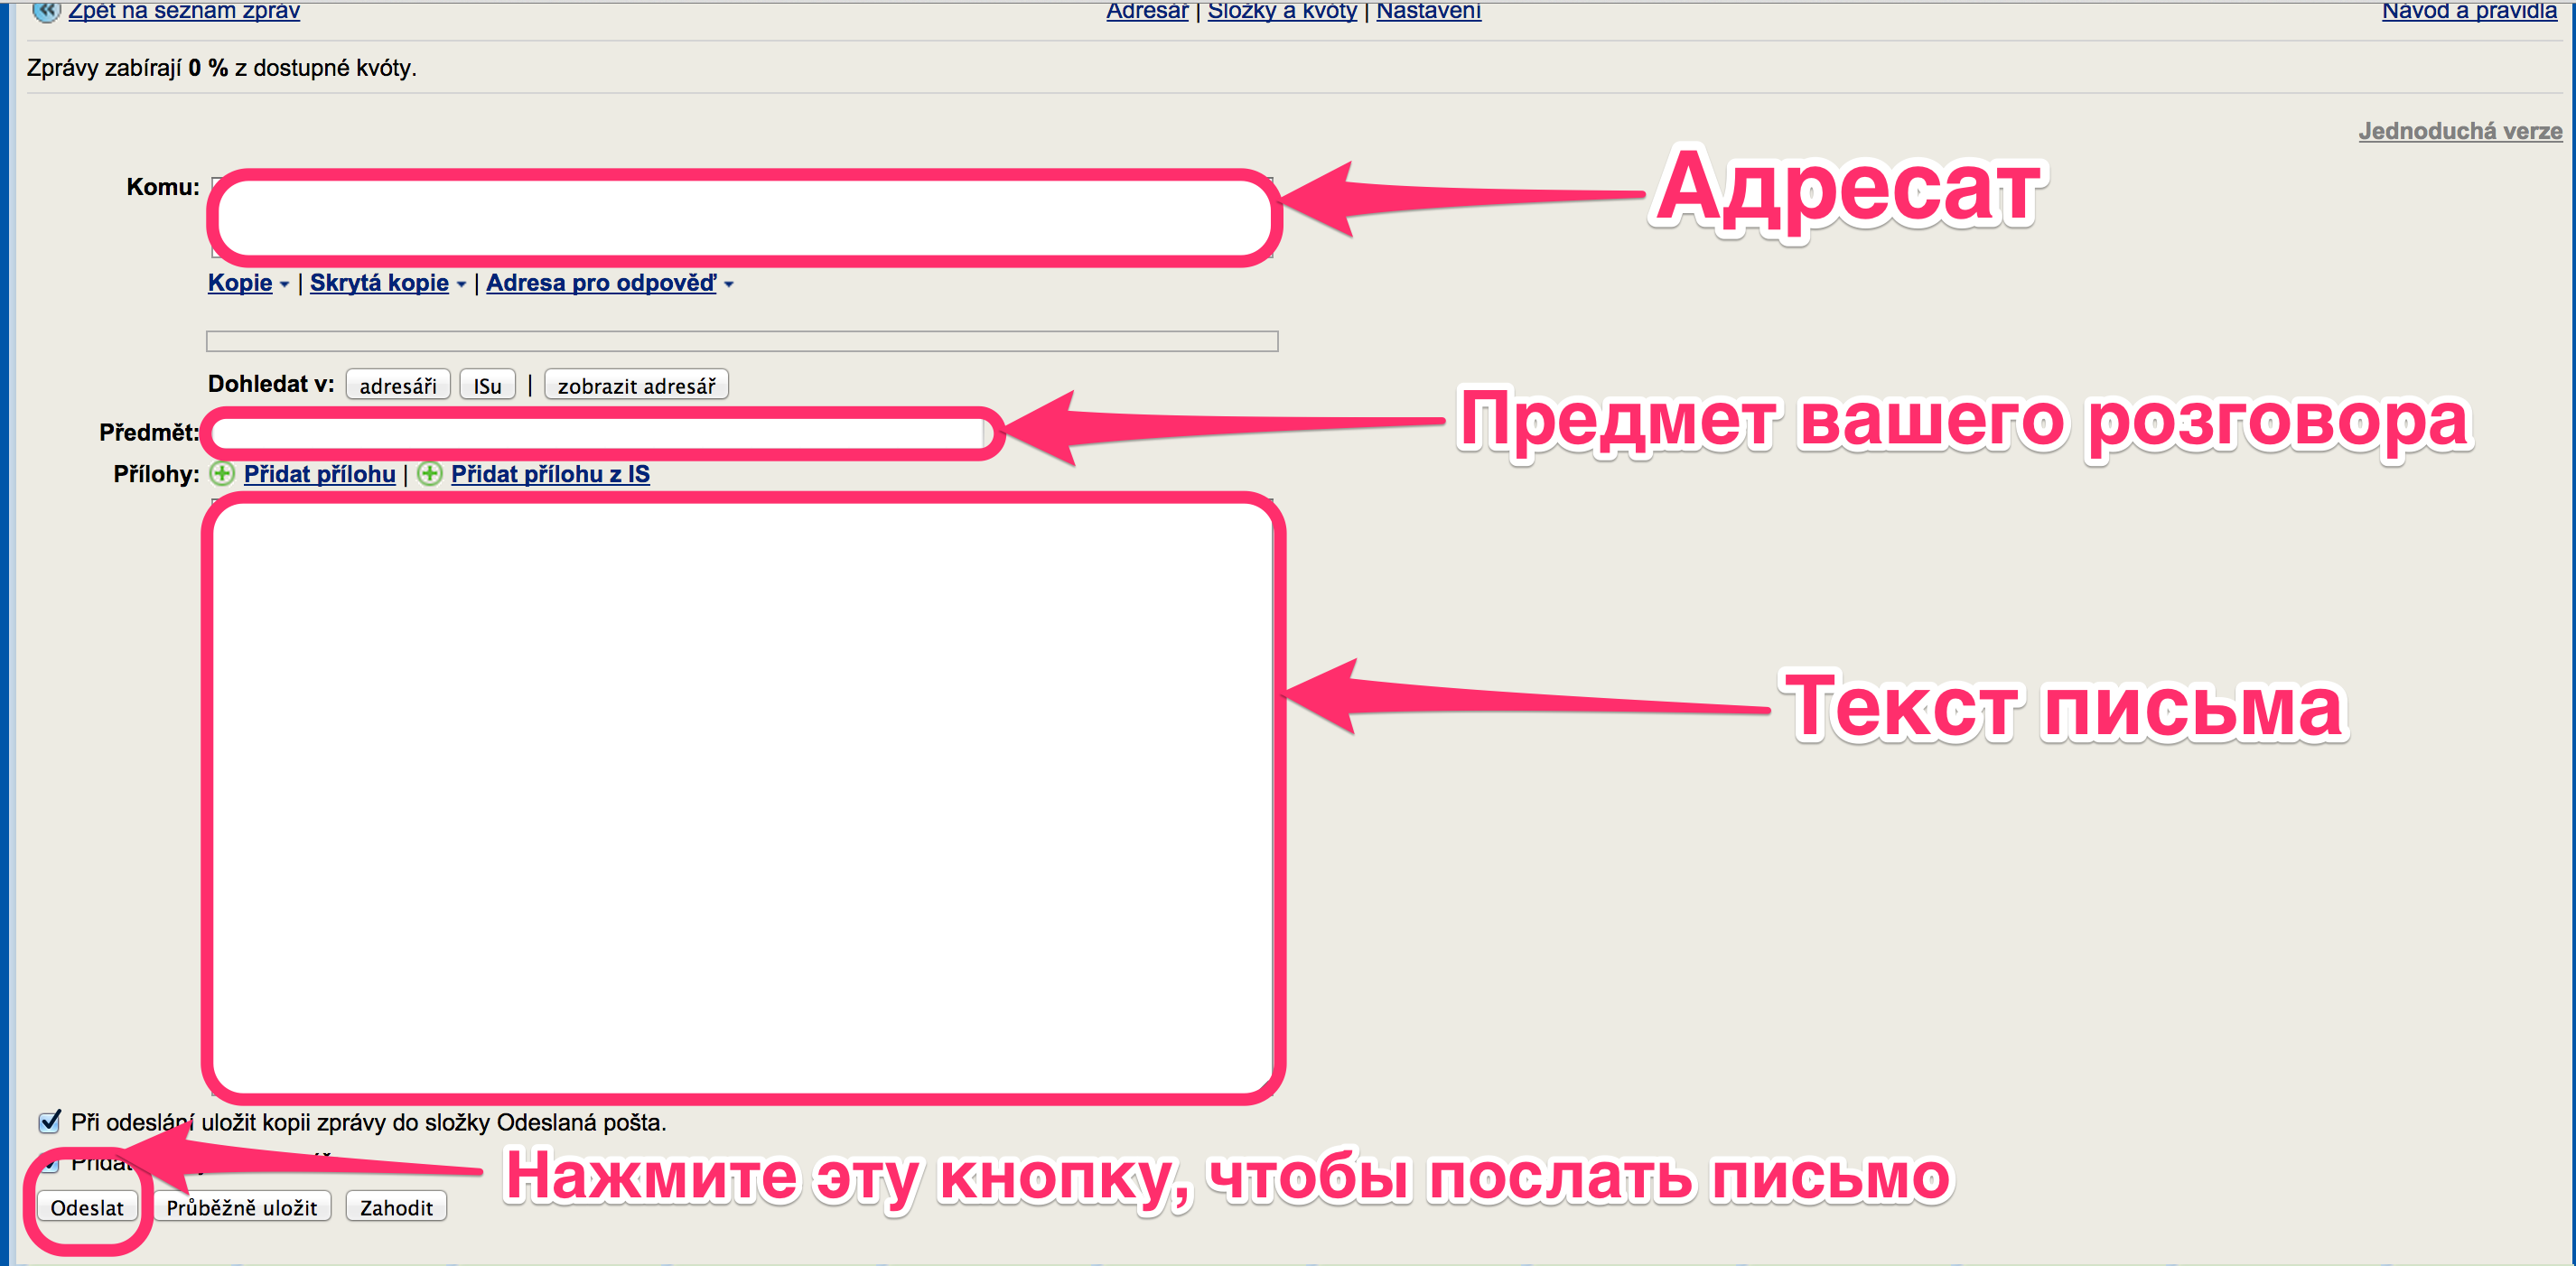
\includegraphics[width=\textwidth]{s10} \\

Пример письма.

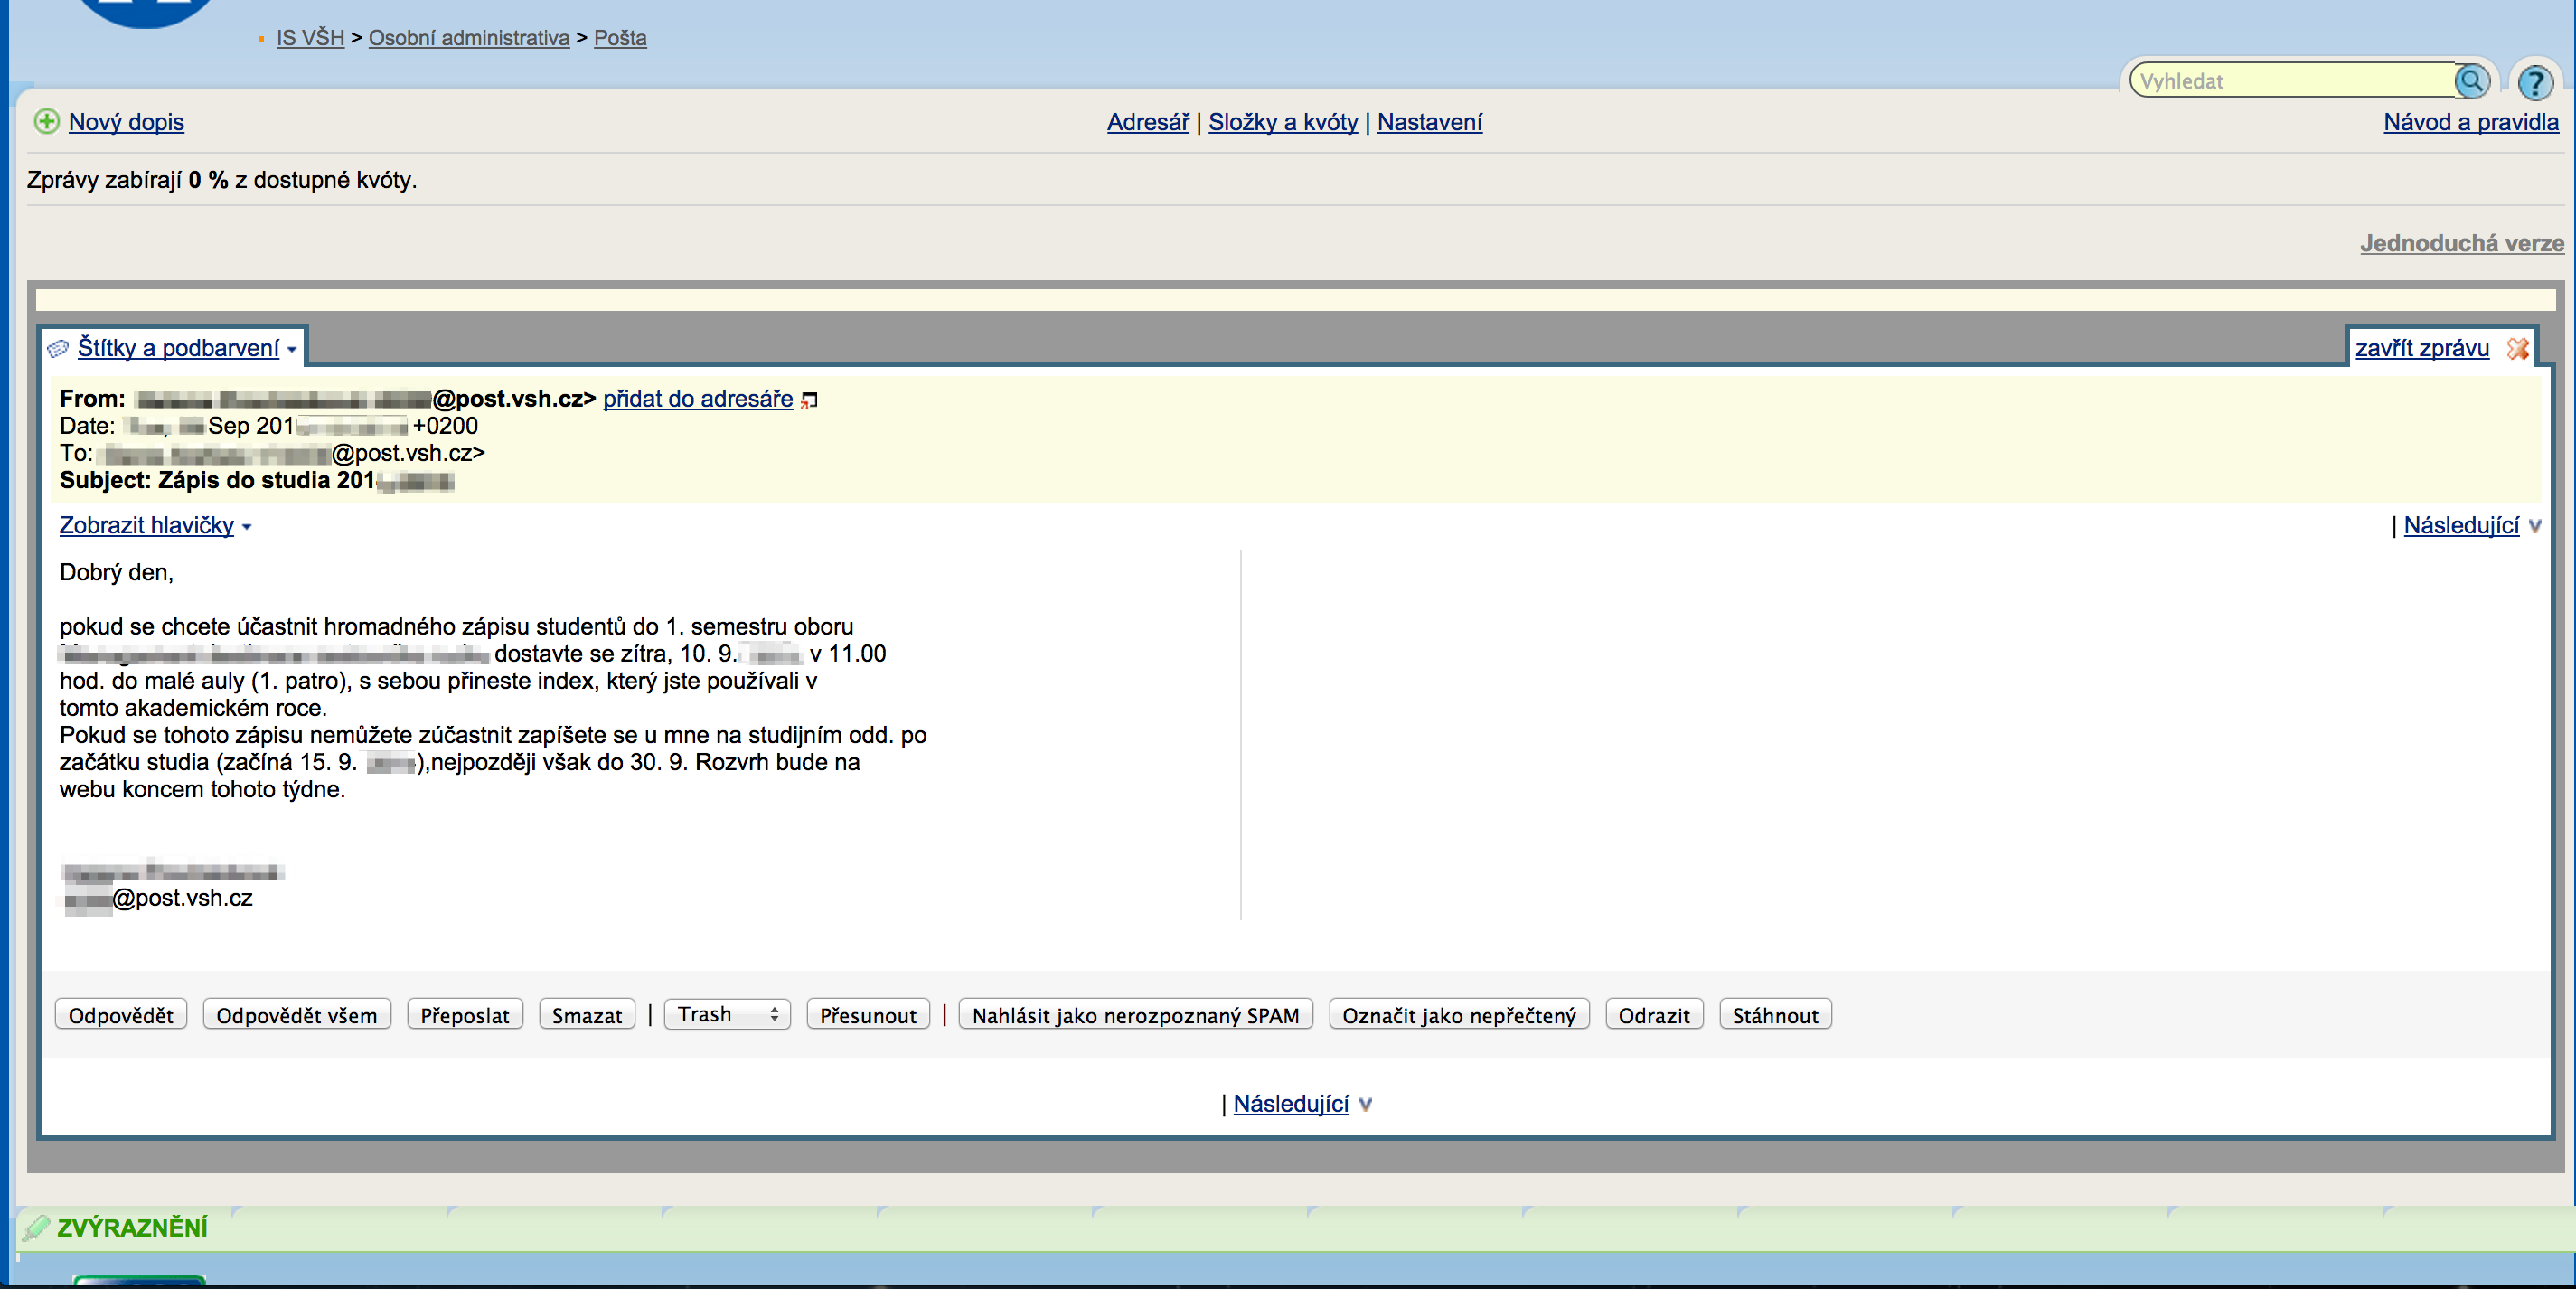
\includegraphics[width=\textwidth]{s10-1}

\newpage

\section{Как найти важную информацию}

Почти вся важная информация расположена в разделе 
\href{https://is.vsh.cz/auth/vyveska/}{Vývěska} \\

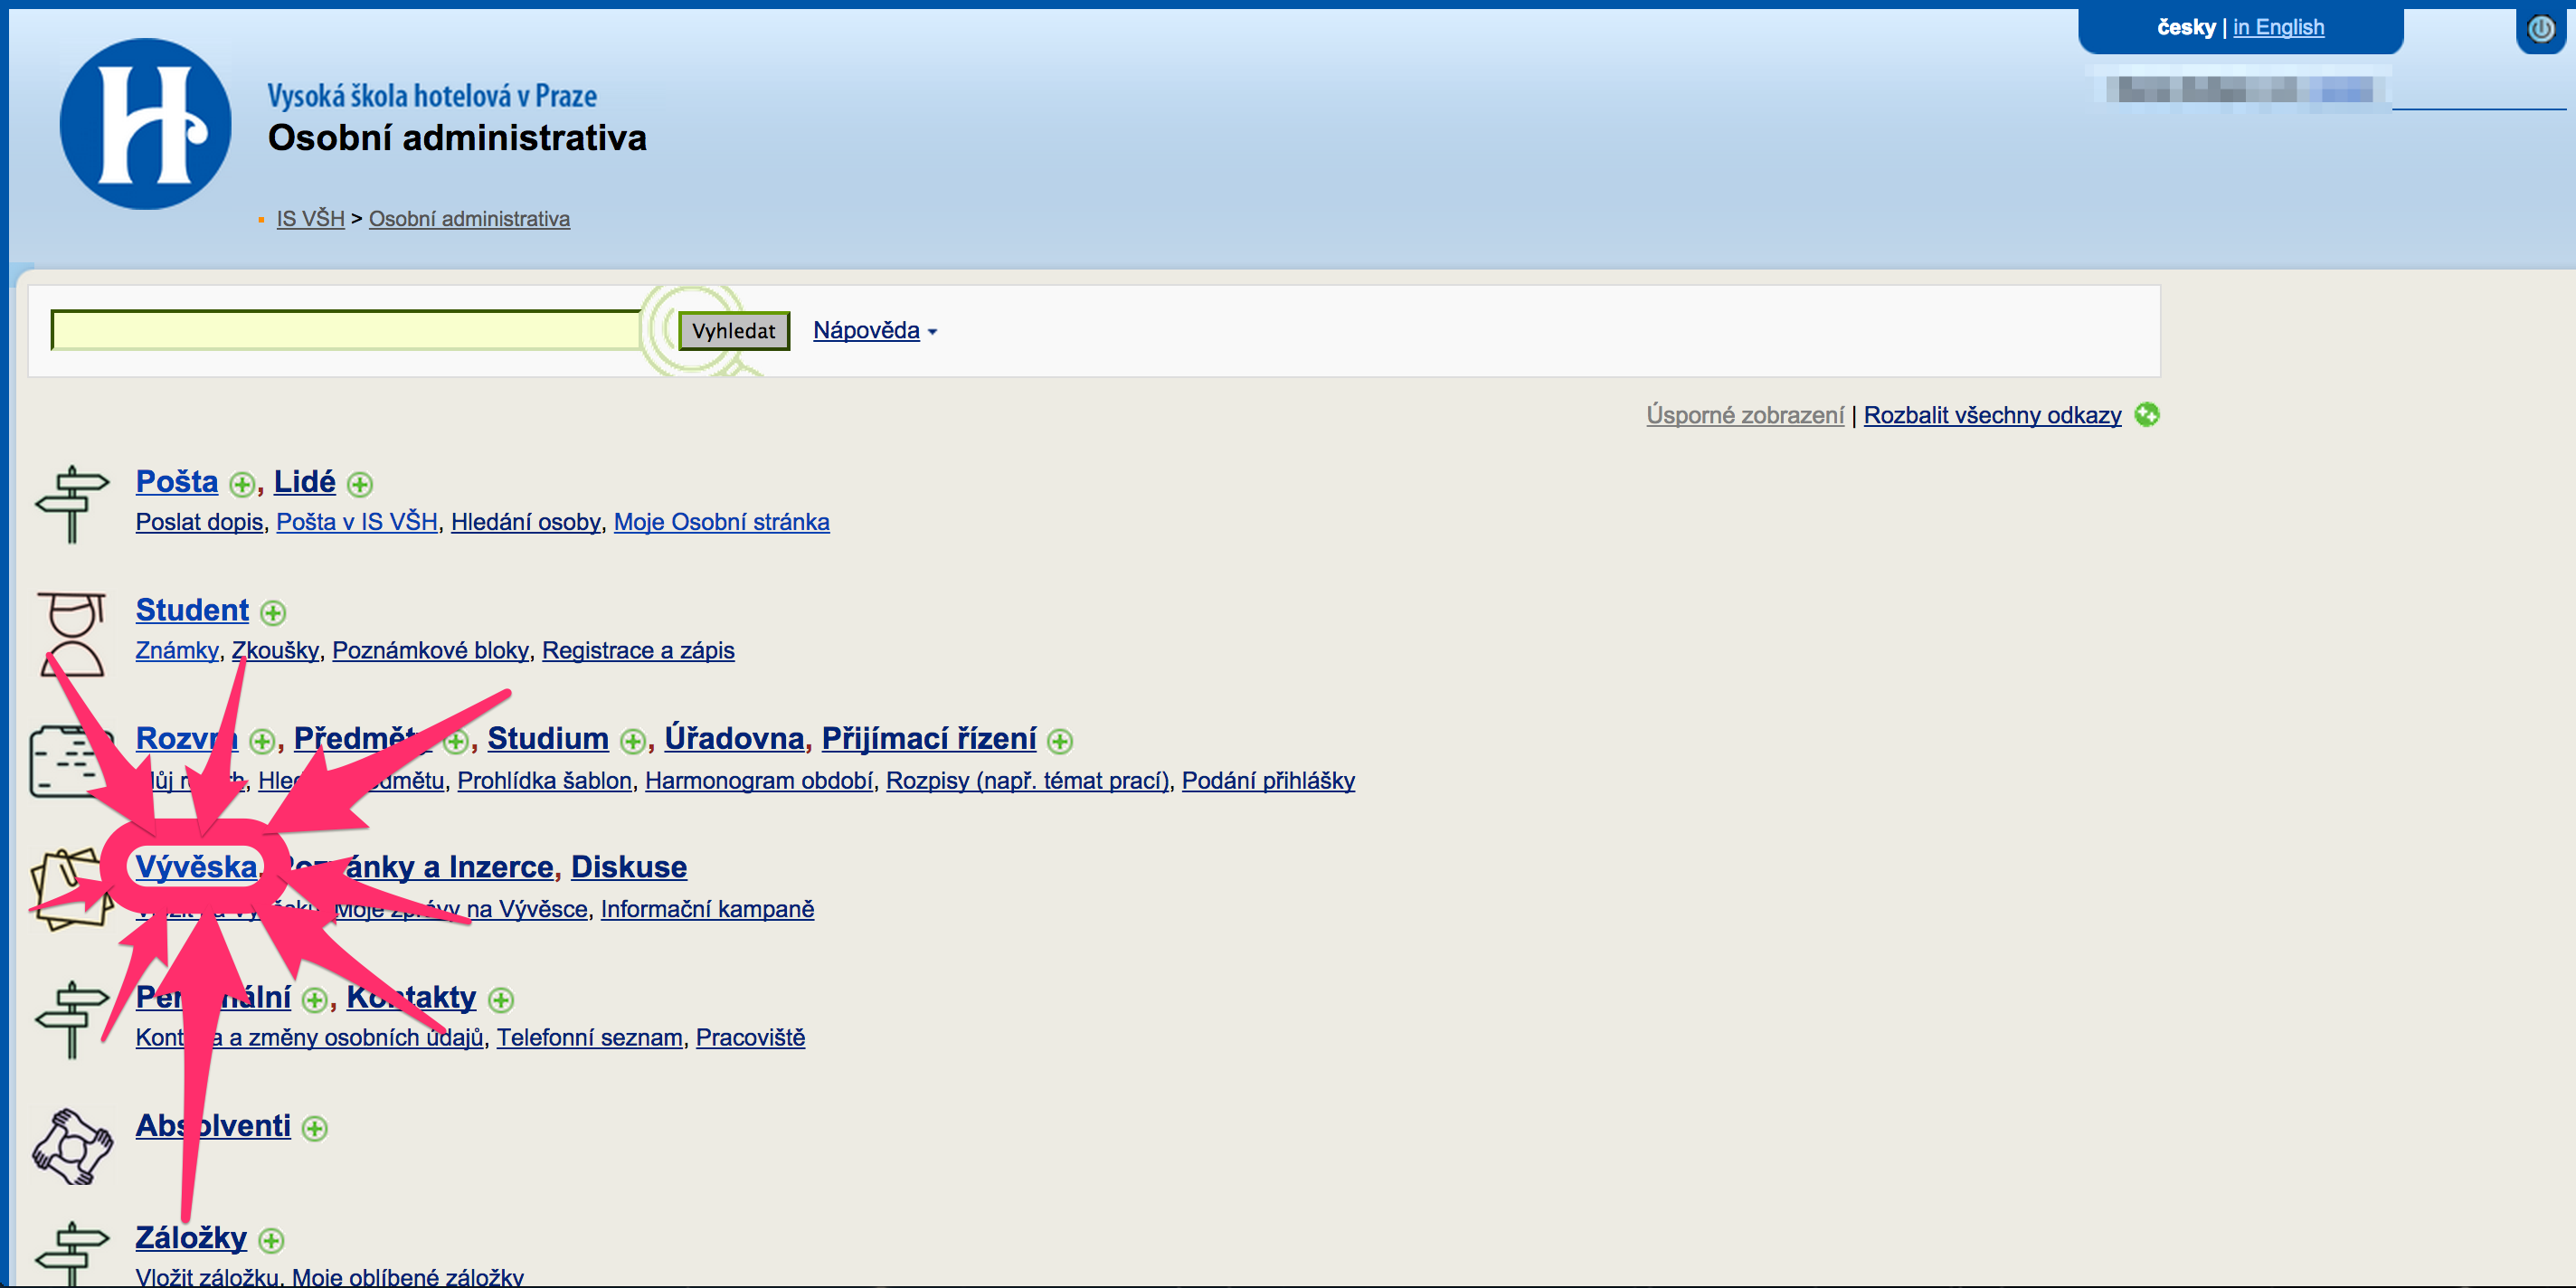
\includegraphics[width=\textwidth]{s11} \\

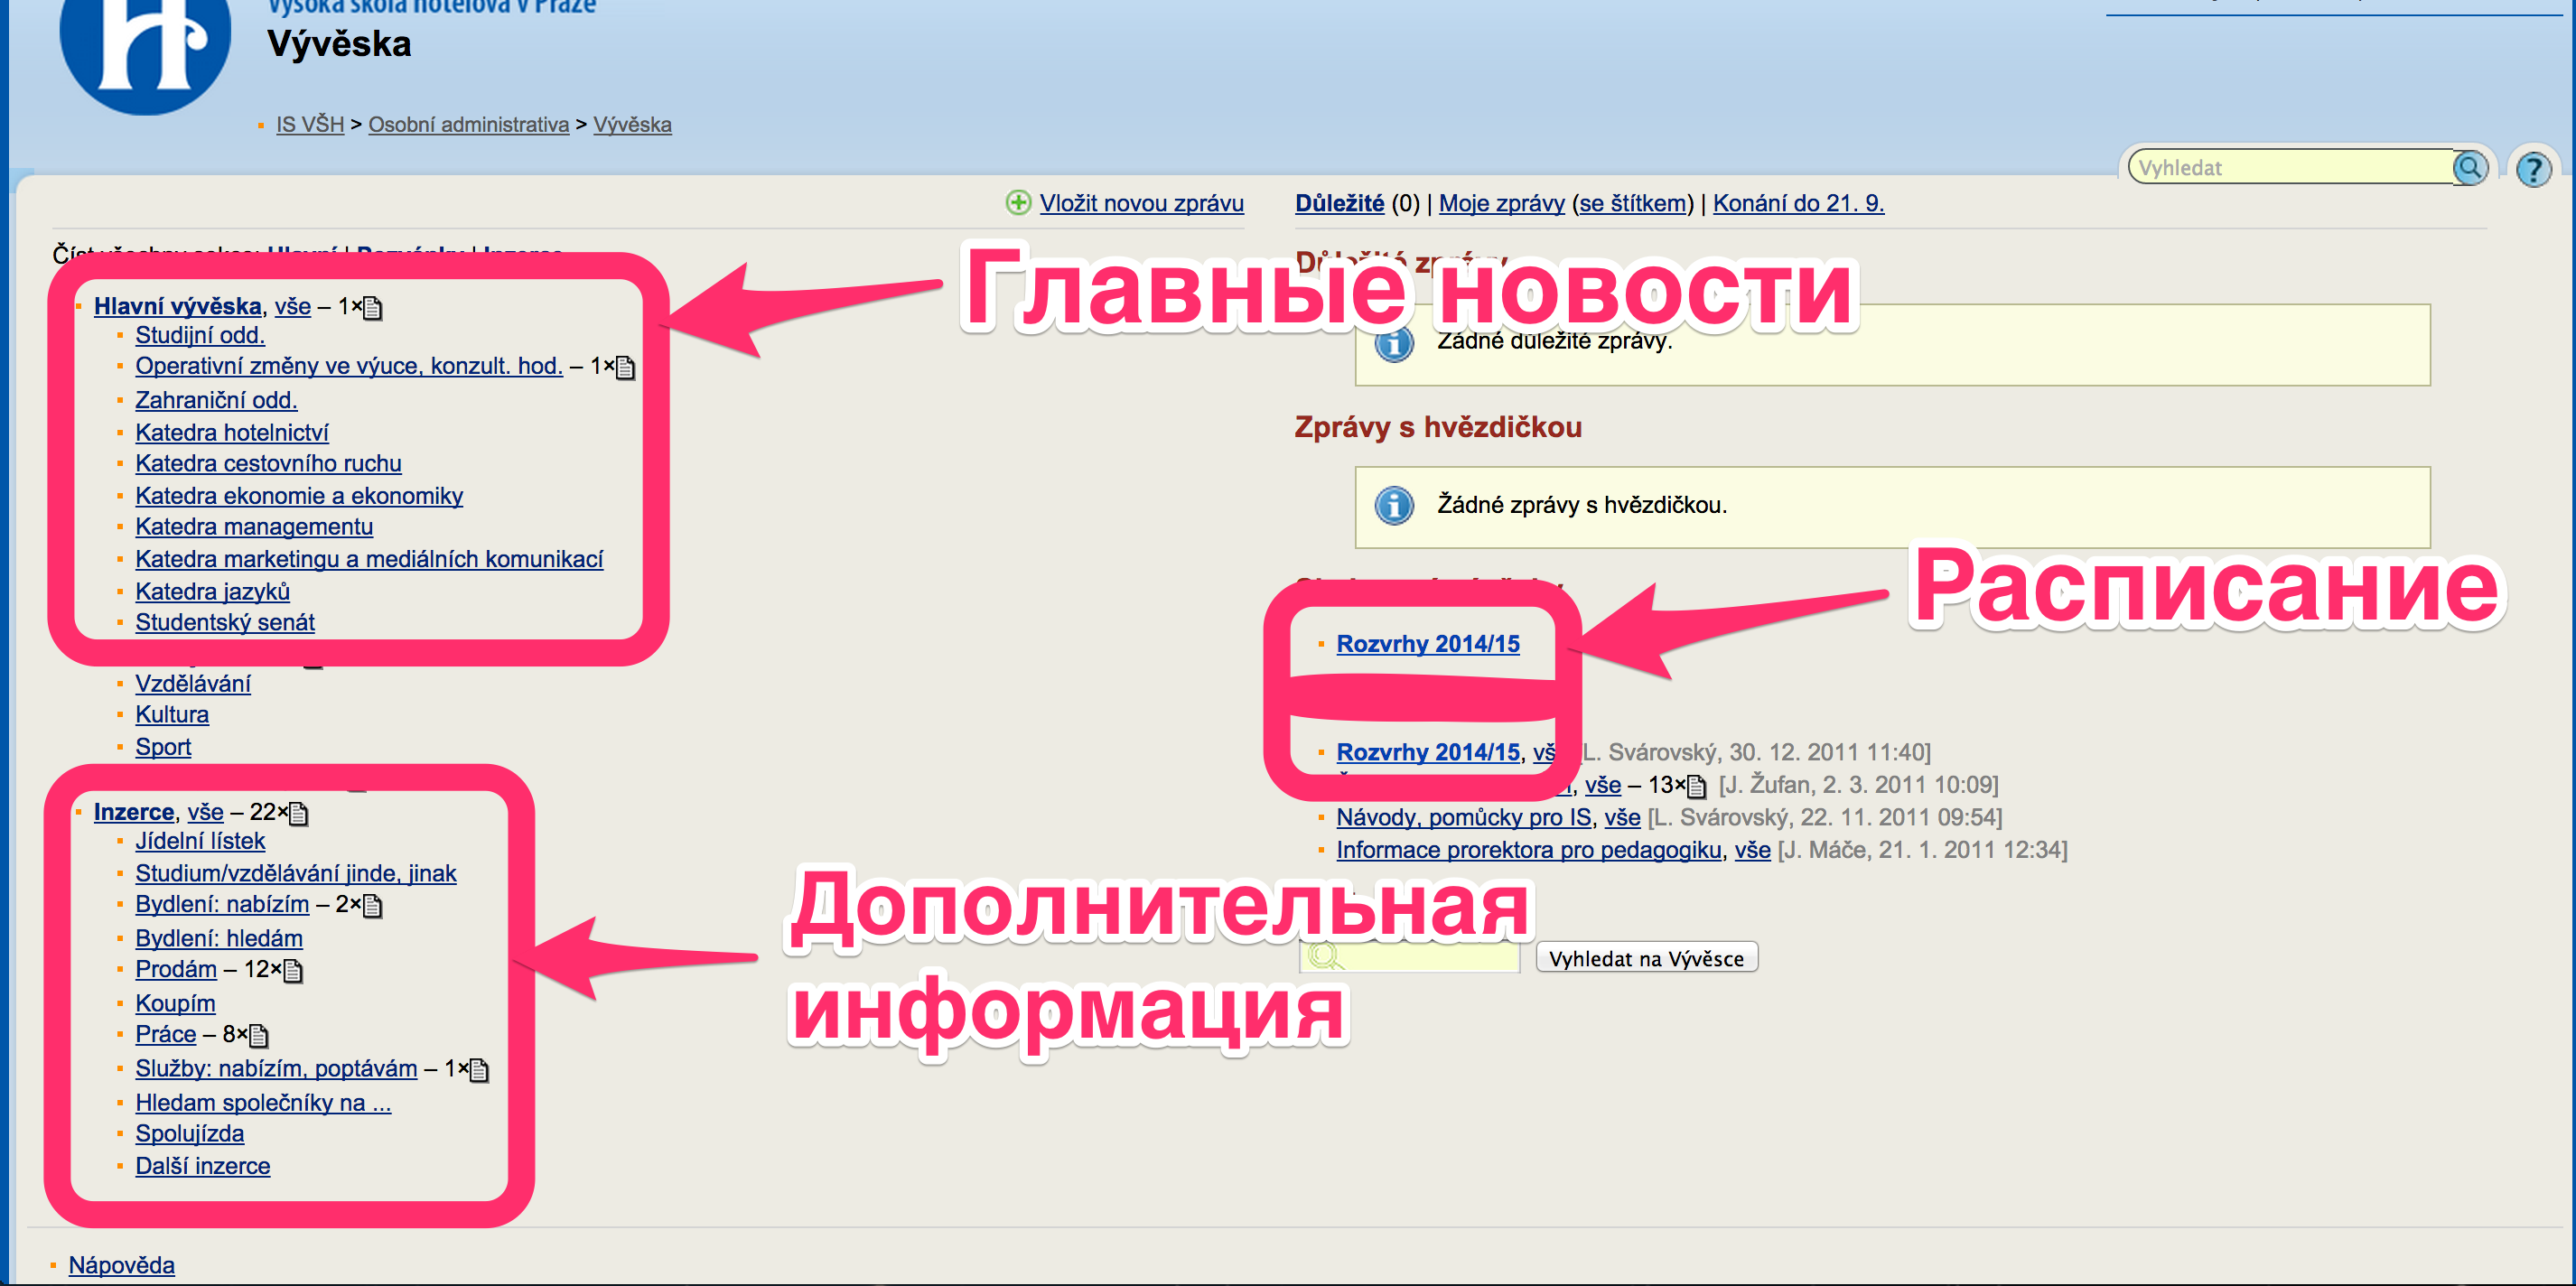
\includegraphics[width=\textwidth]{s12} \\

На этой странице можно найти сразу две ссылки на расписание, \textbf{Hlavní vývěska} 
слева вверху показывает новости студенческого отделения, факультетов, сената и тд.
Никогда не забывайте лишний раз проверить этот раздел.
Все критически важные новости находятся здесь.

Под \textbf{Hlavní vývěskou} находится раздел \textbf{Inzerce}, в 
котором можно найти информацию о работе, 
покупке/продаже различных учебных материалов и даже аренде квартир.

\newpage

\subsection{Расписание}
Чтобы узнать своё расписание, вам надо зайти в раздел \href{https://is.vsh.cz/auth/vyveska/}{Vývěska}
и нажать на одну из двух ссылок, которые называются \textbf{Rozvrhy} \\

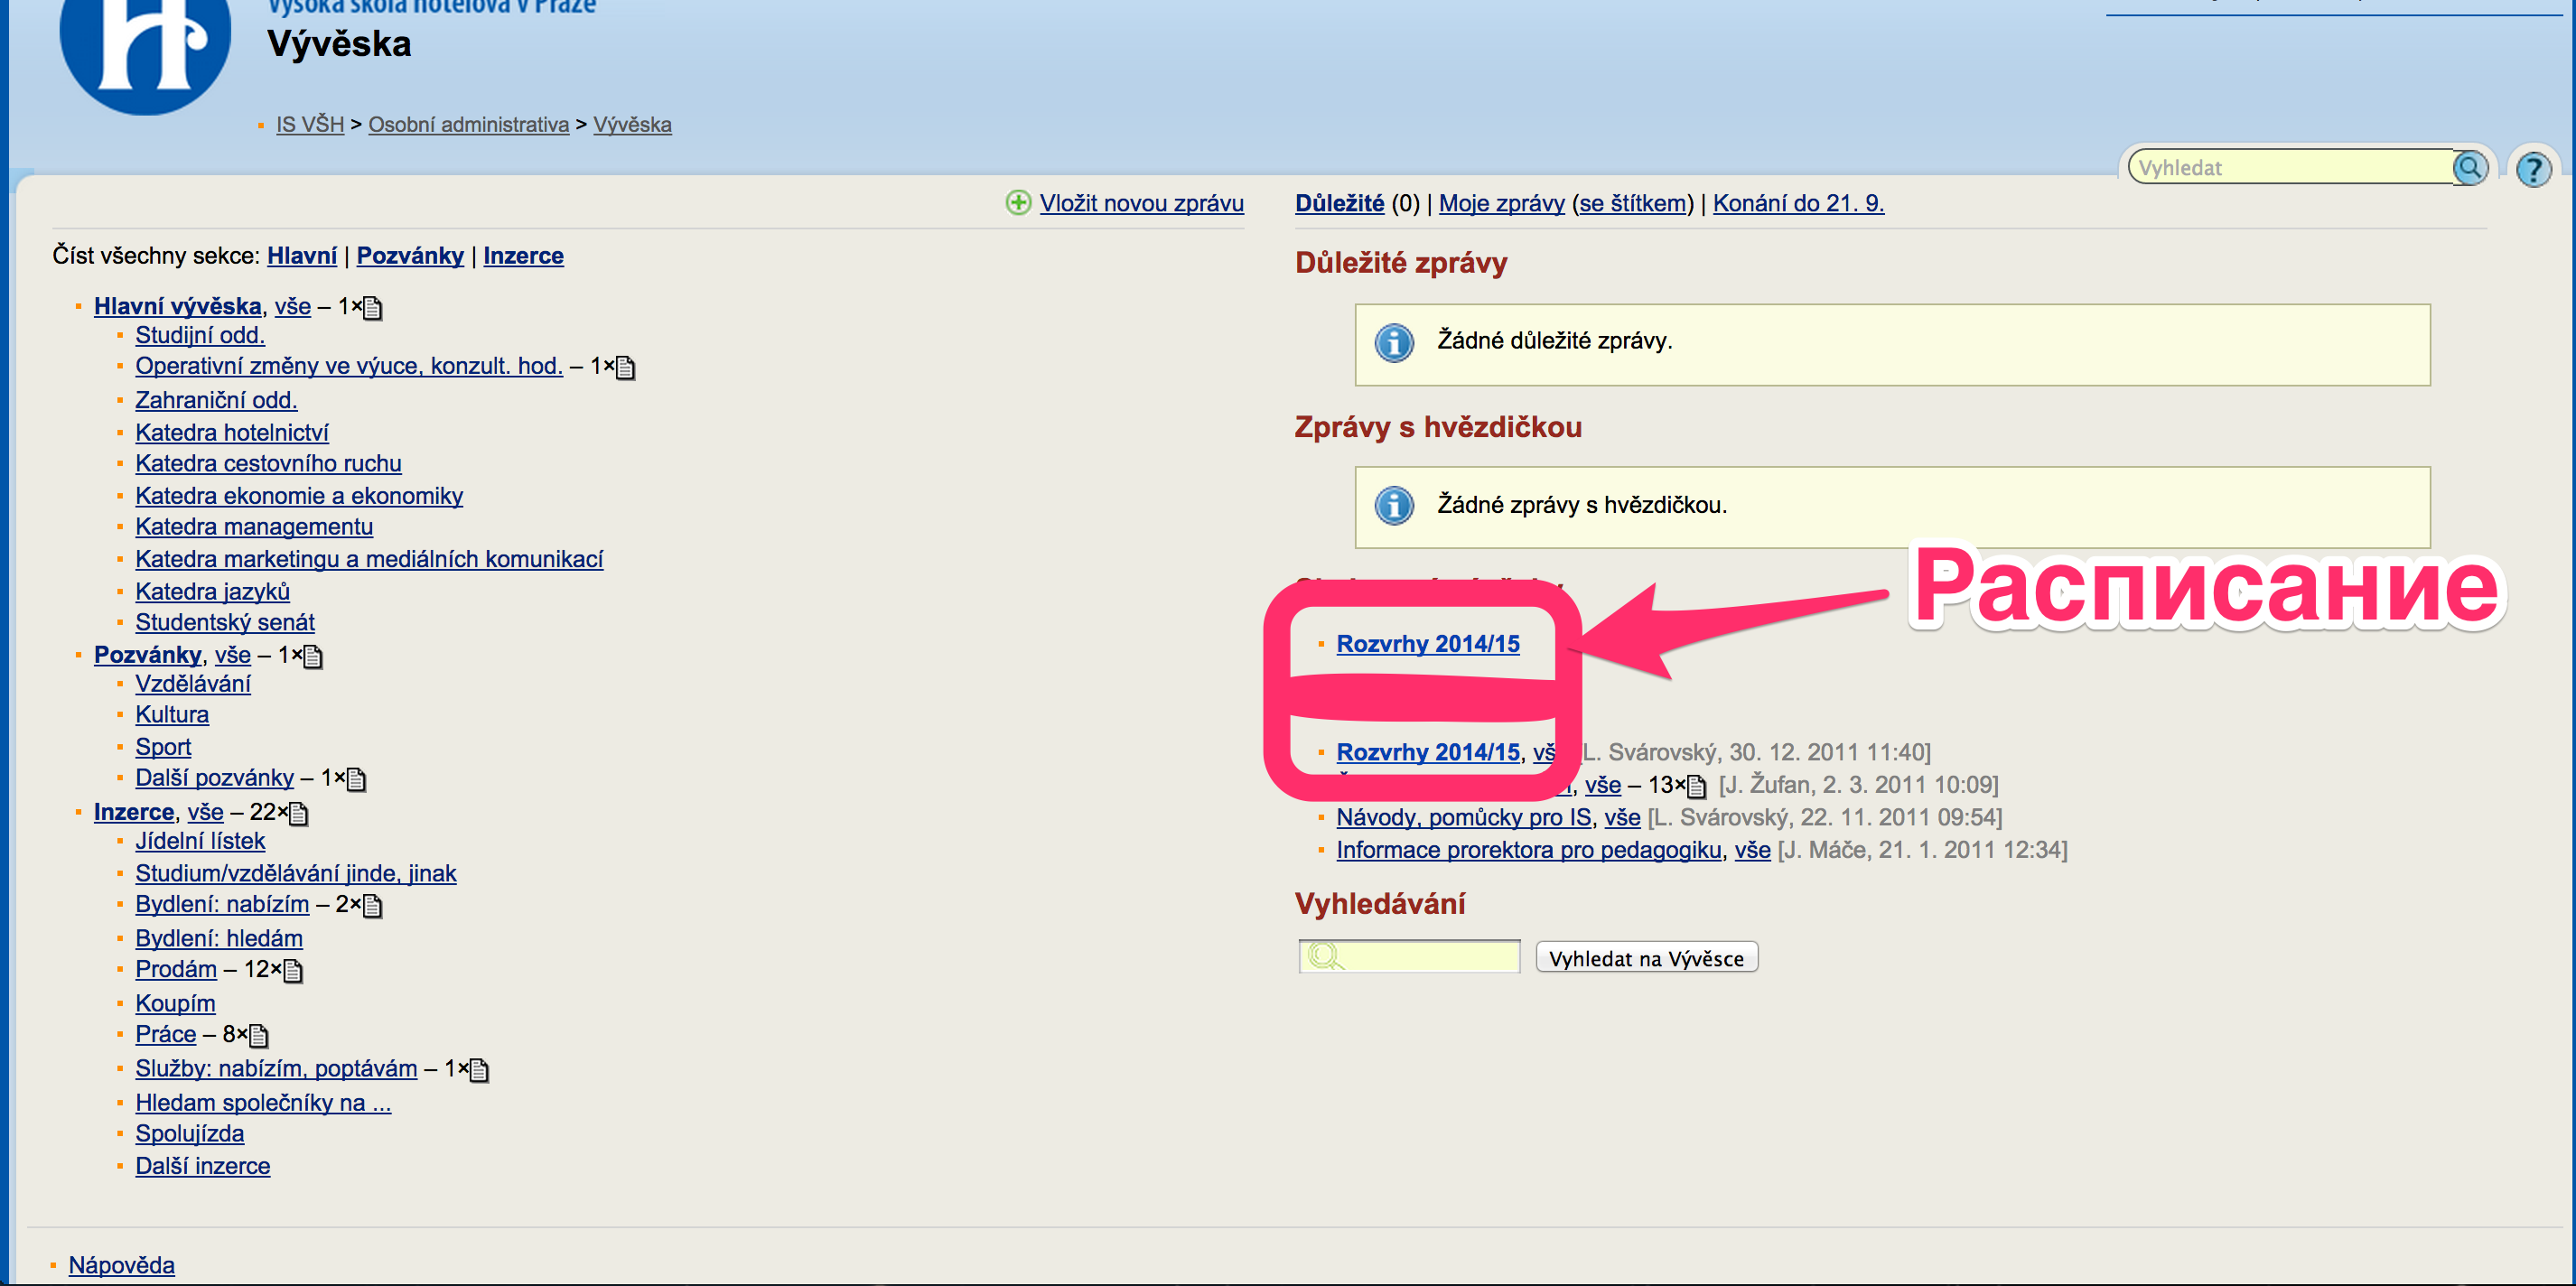
\includegraphics[width=\textwidth]{s13} \\

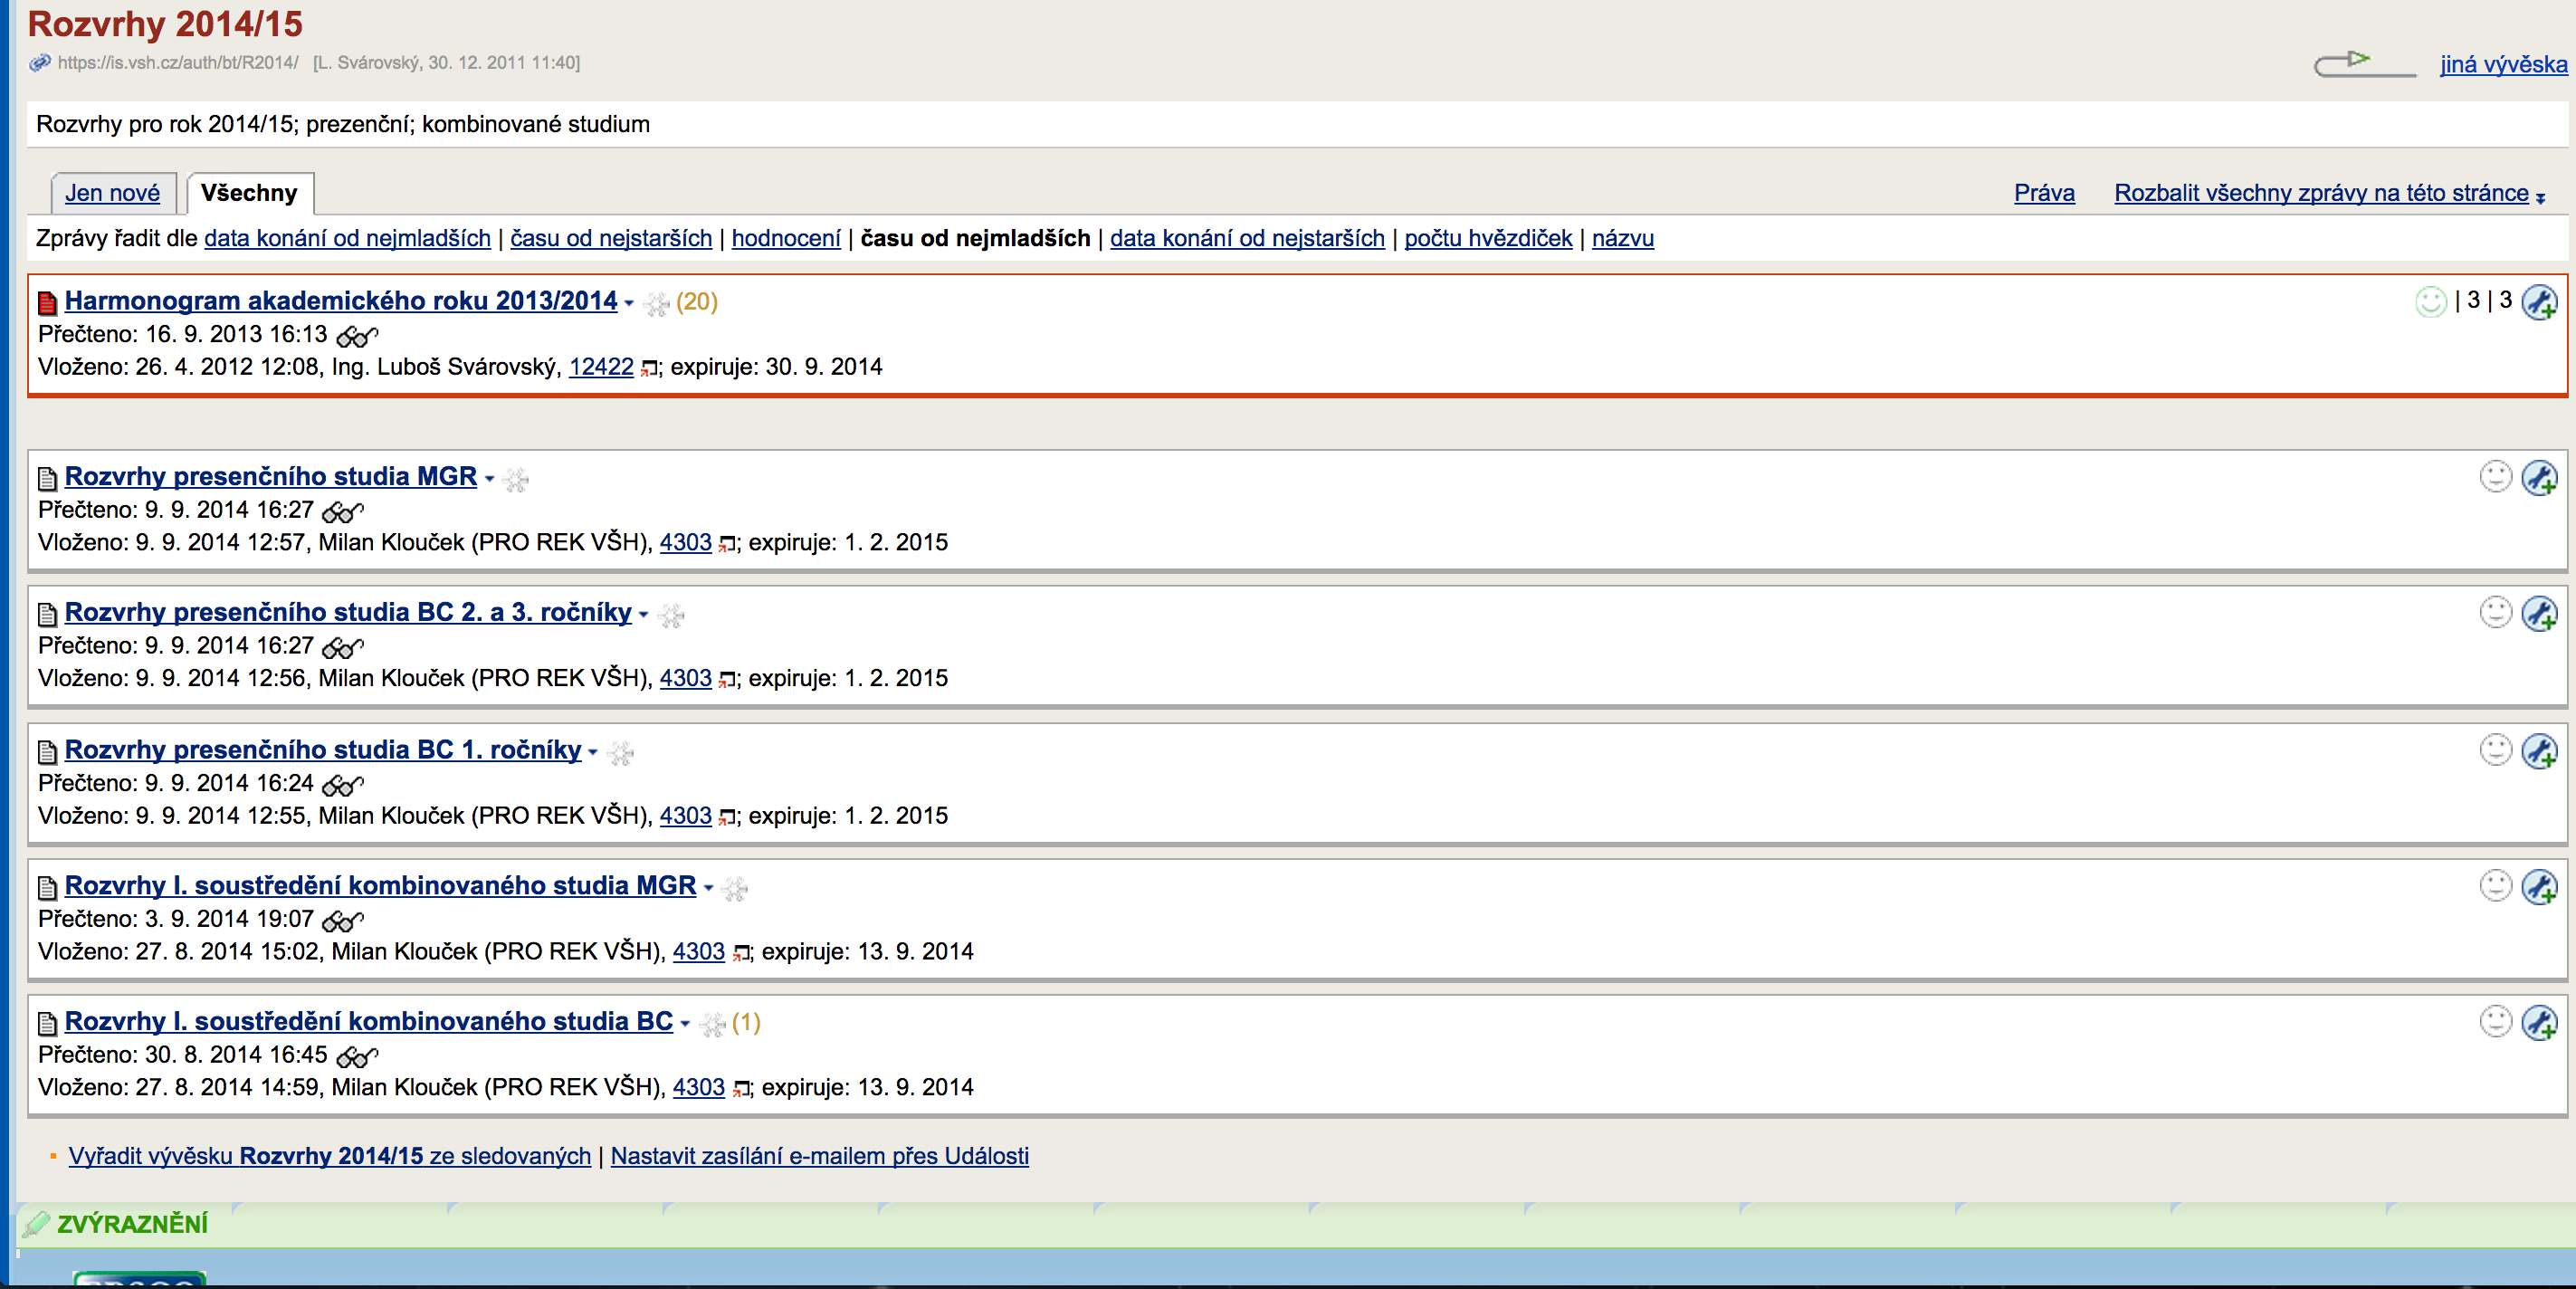
\includegraphics[width=\textwidth]{s14} \\

\newpage

Здесь находятся расписания ВСЕХ факультетов, годов и отделений, так что вы должны
точно знать, какое именно расписание вам необходимо. Никакой удобной навигации
для такого случая не предусмотрено. \\

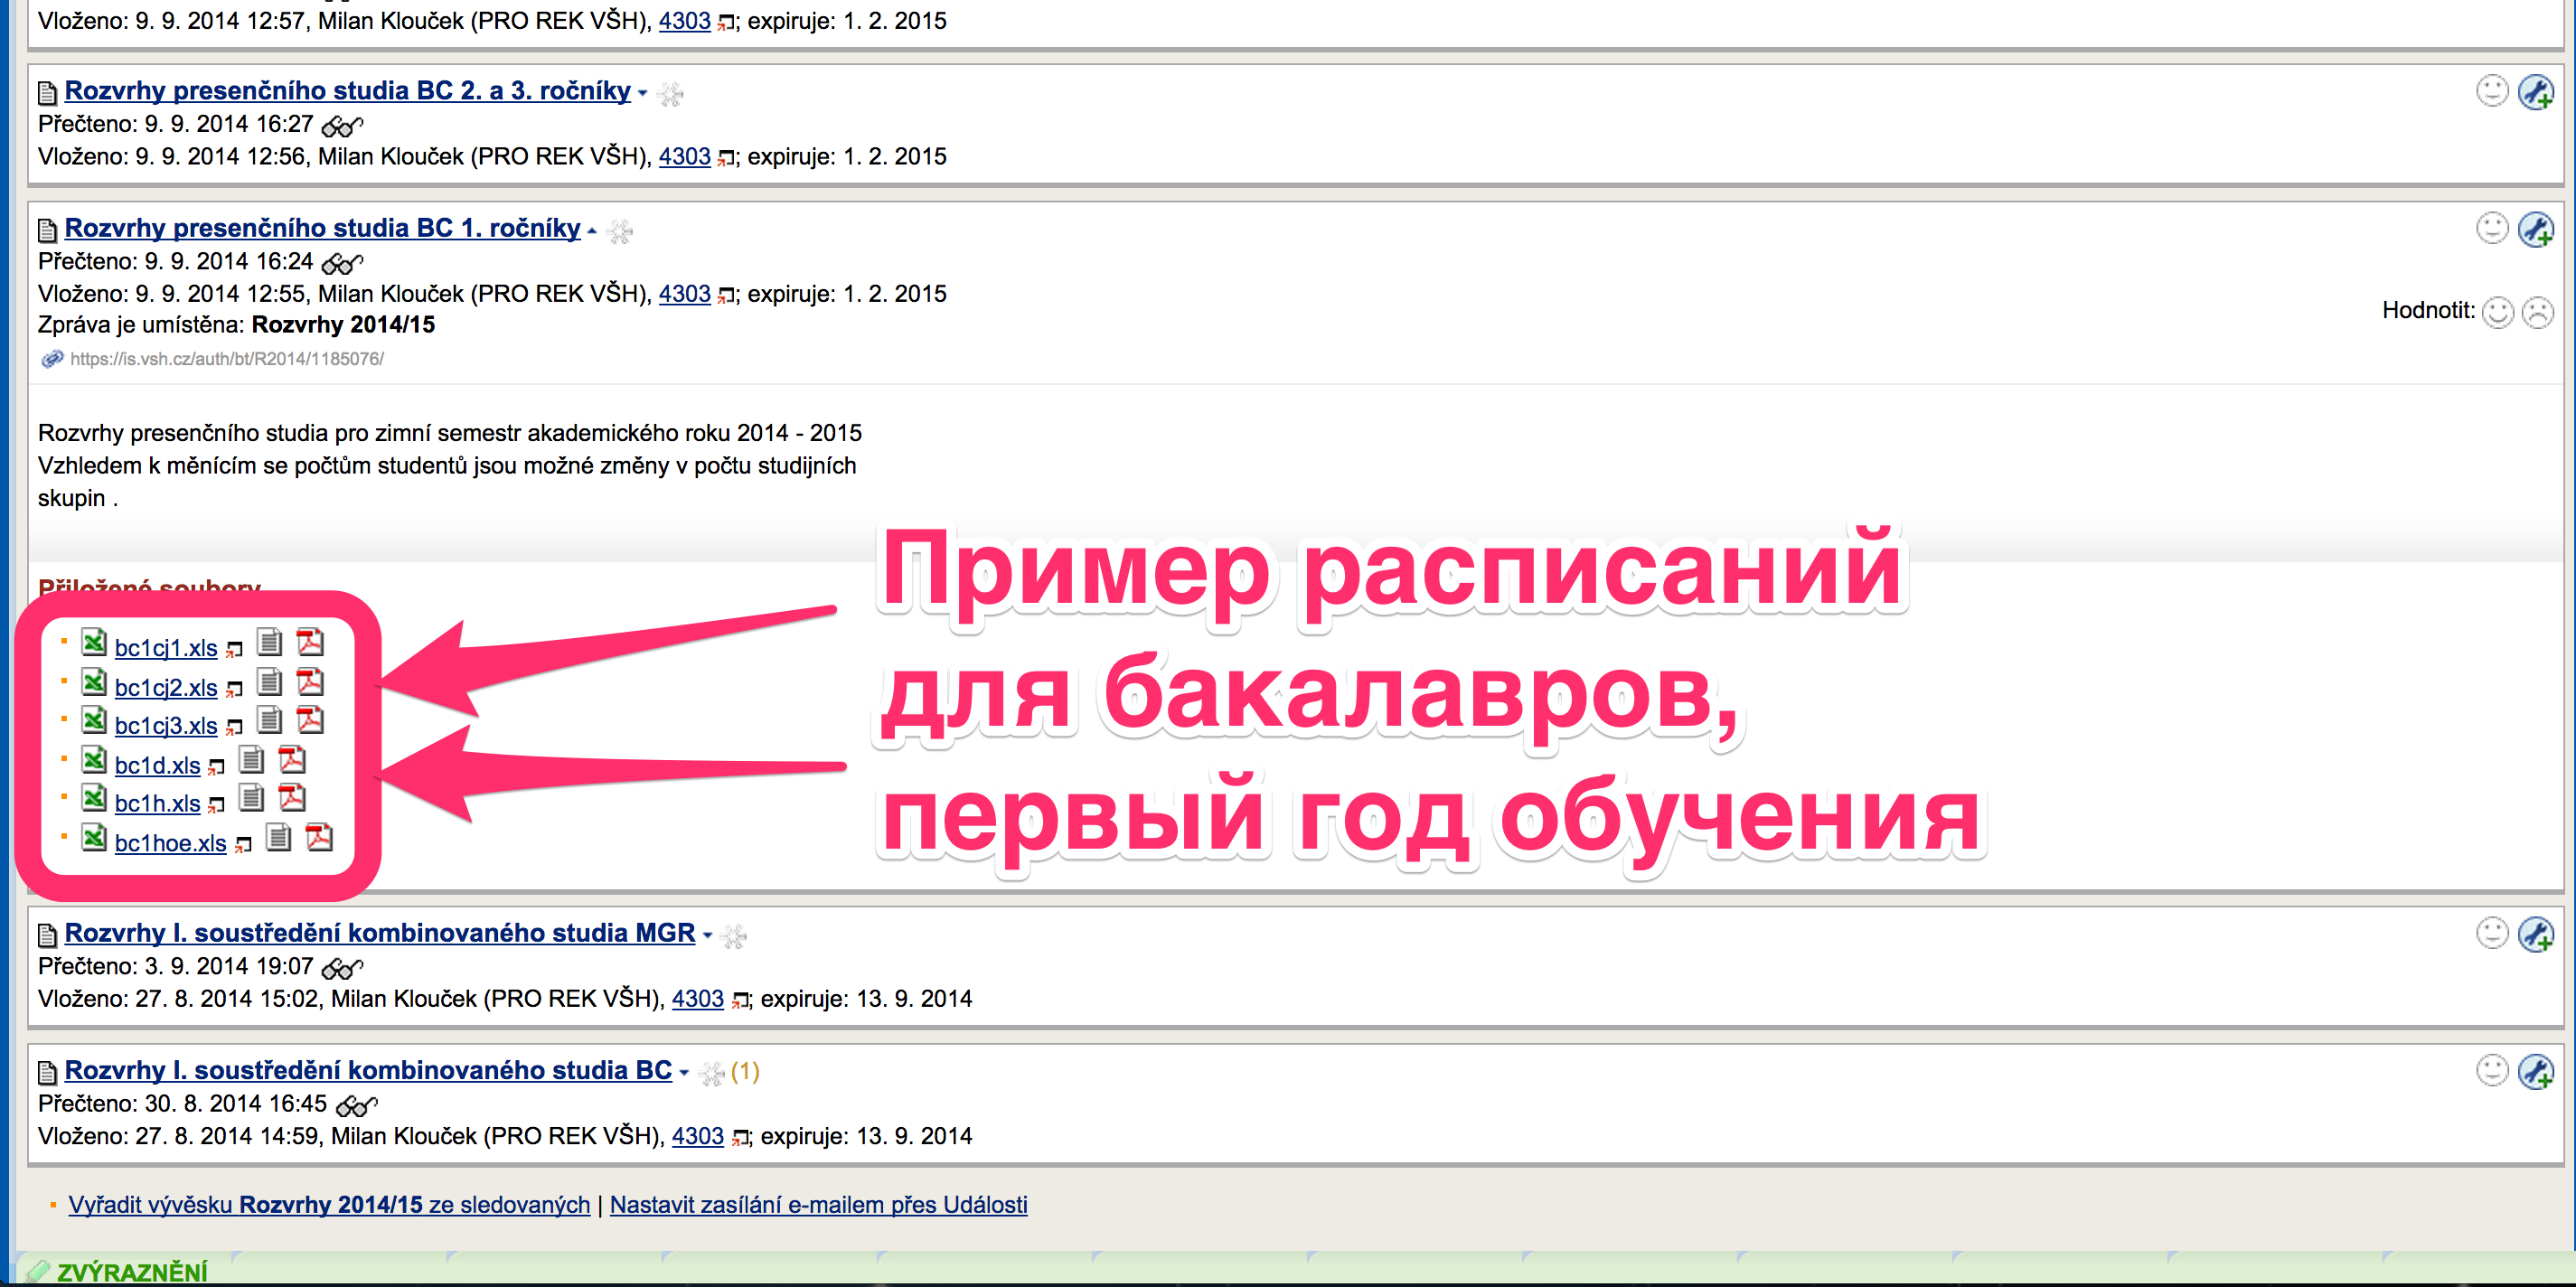
\includegraphics[width=\textwidth]{s15}

\subsection{Пример расписания}

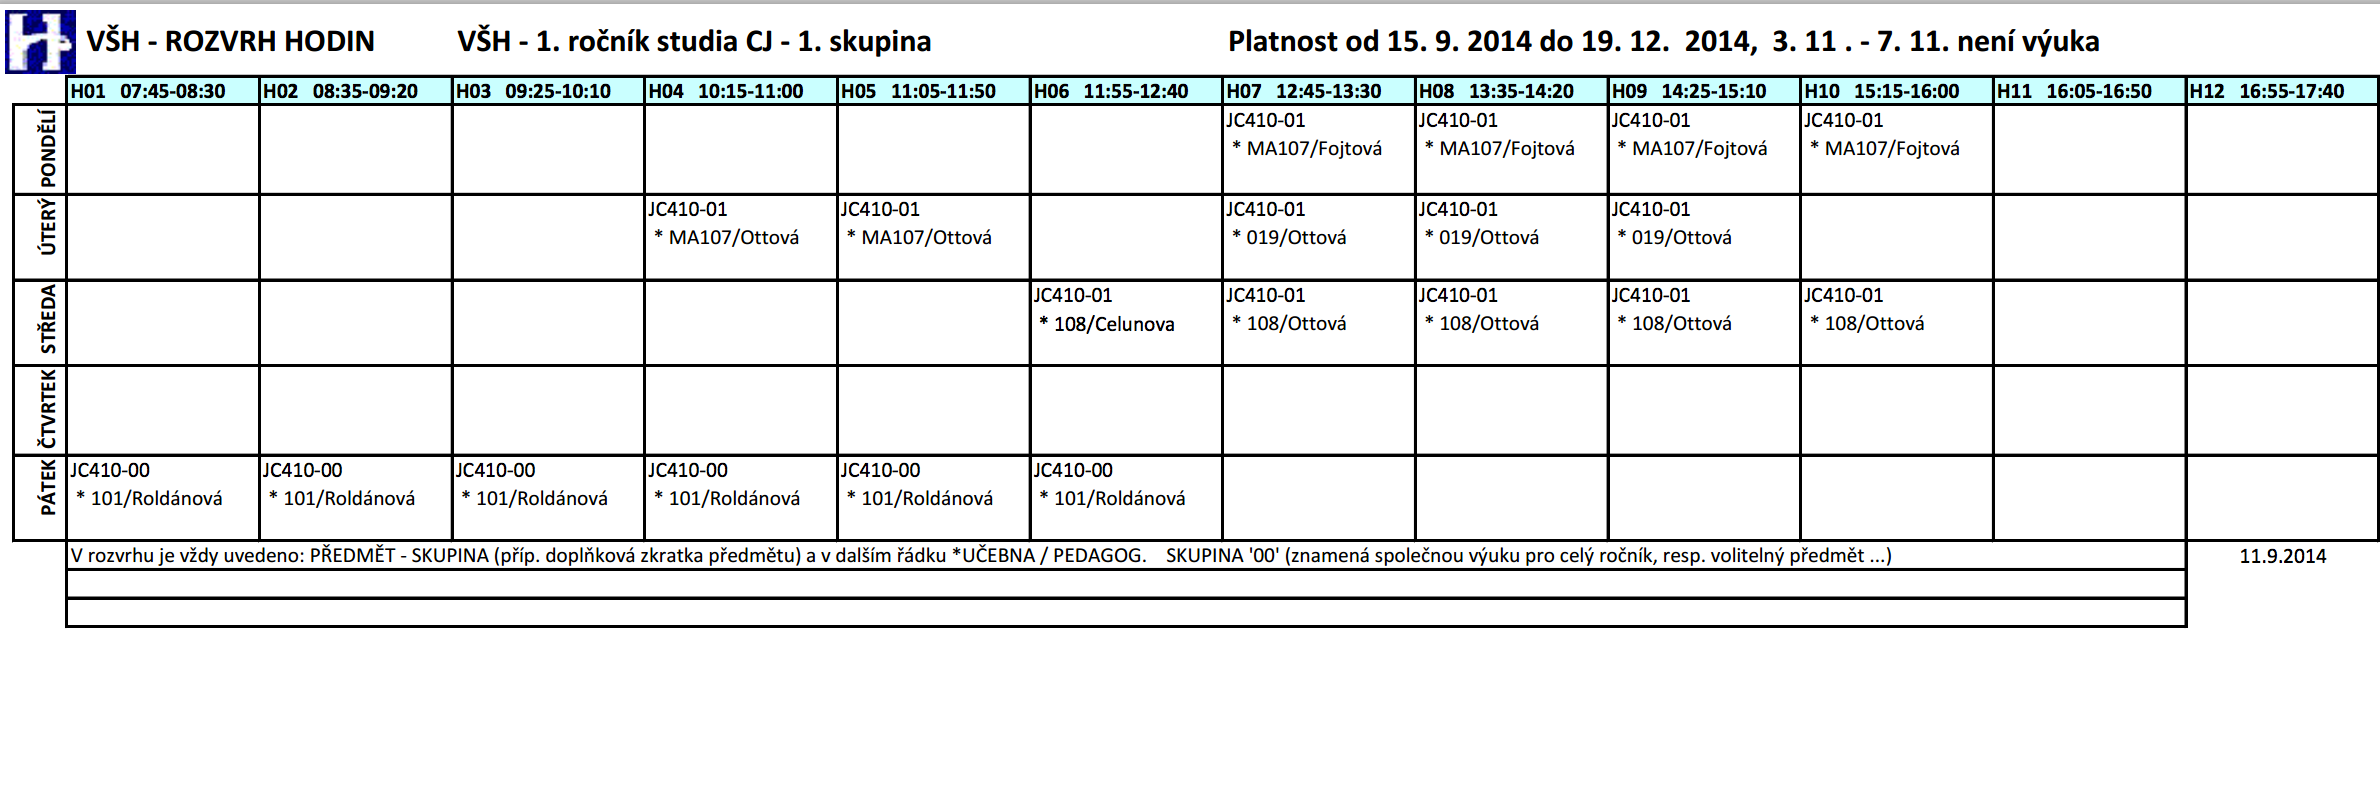
\includegraphics[width=\textwidth]{s16} \\

\newpage

\section{Оценки и оплата за обучение}

Теперь рассмотрим раздел \href{https://is.vsh.cz/auth/student/}{Student}. \\

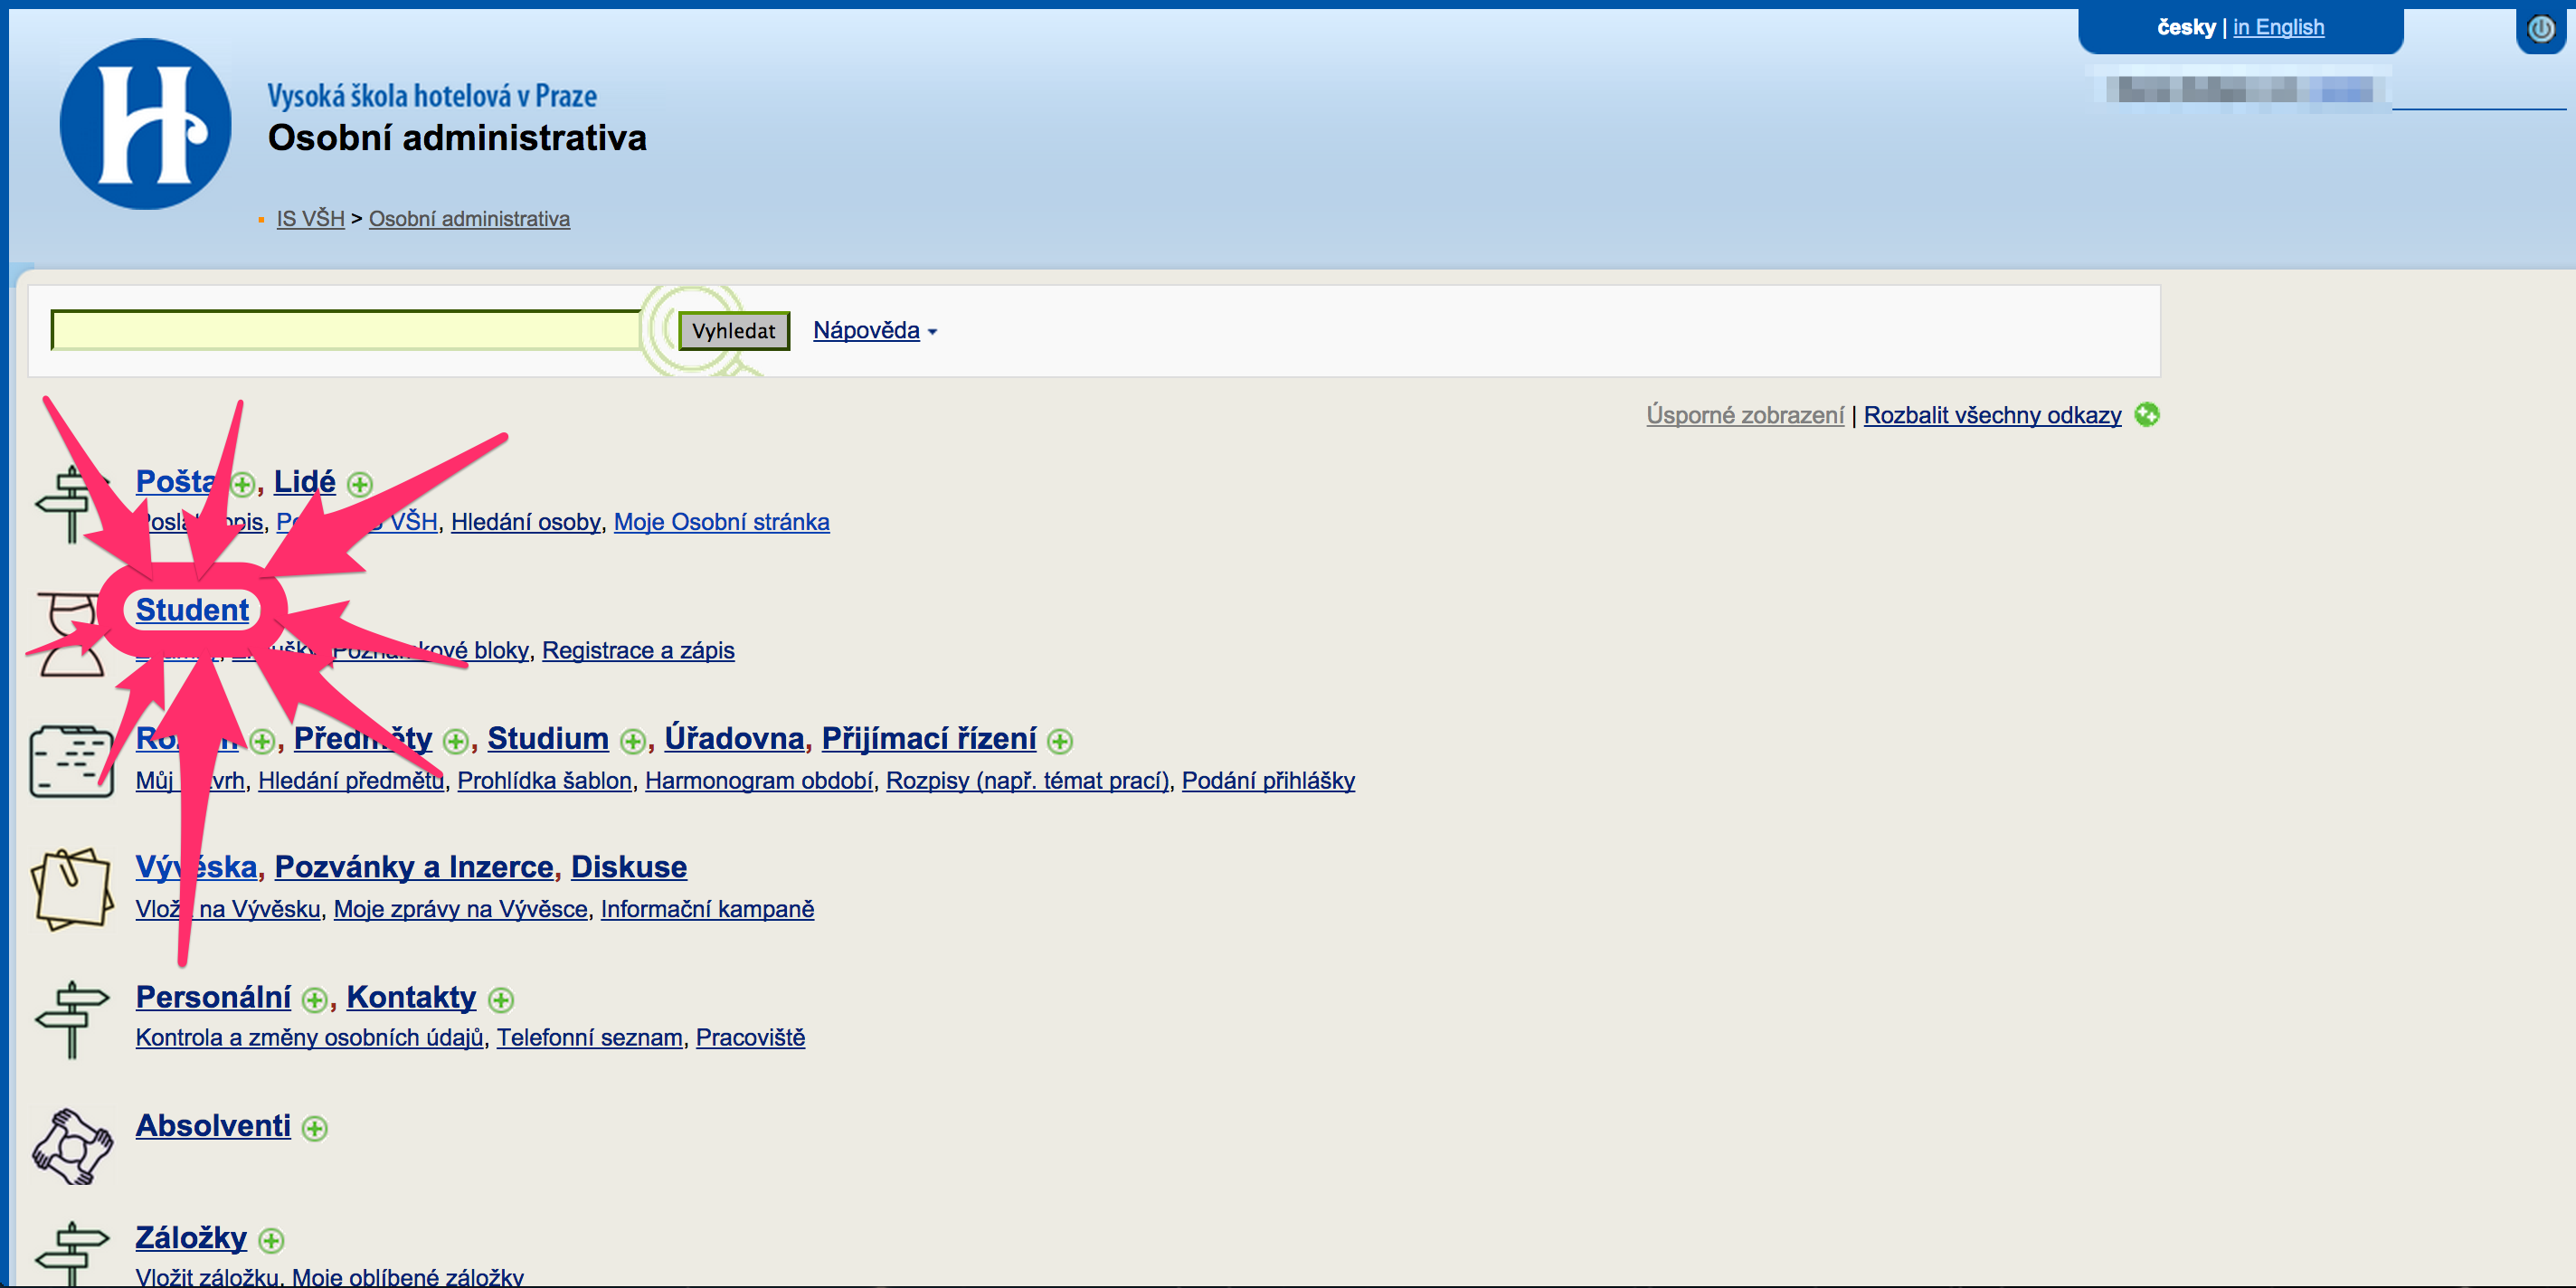
\includegraphics[width=\textwidth]{s17} \\

В этом разделе вы увидите свои предметы.

Оплату за обучение можно посмотреть, 
нажав на ссылку \textbf{Evidence plateb studenta} справа по центру.

Свои оценки можно посмотреть, 
если нажать 
на ссылку \textbf{Známky za celé studium, získané kredity a stud. průměr}. \\

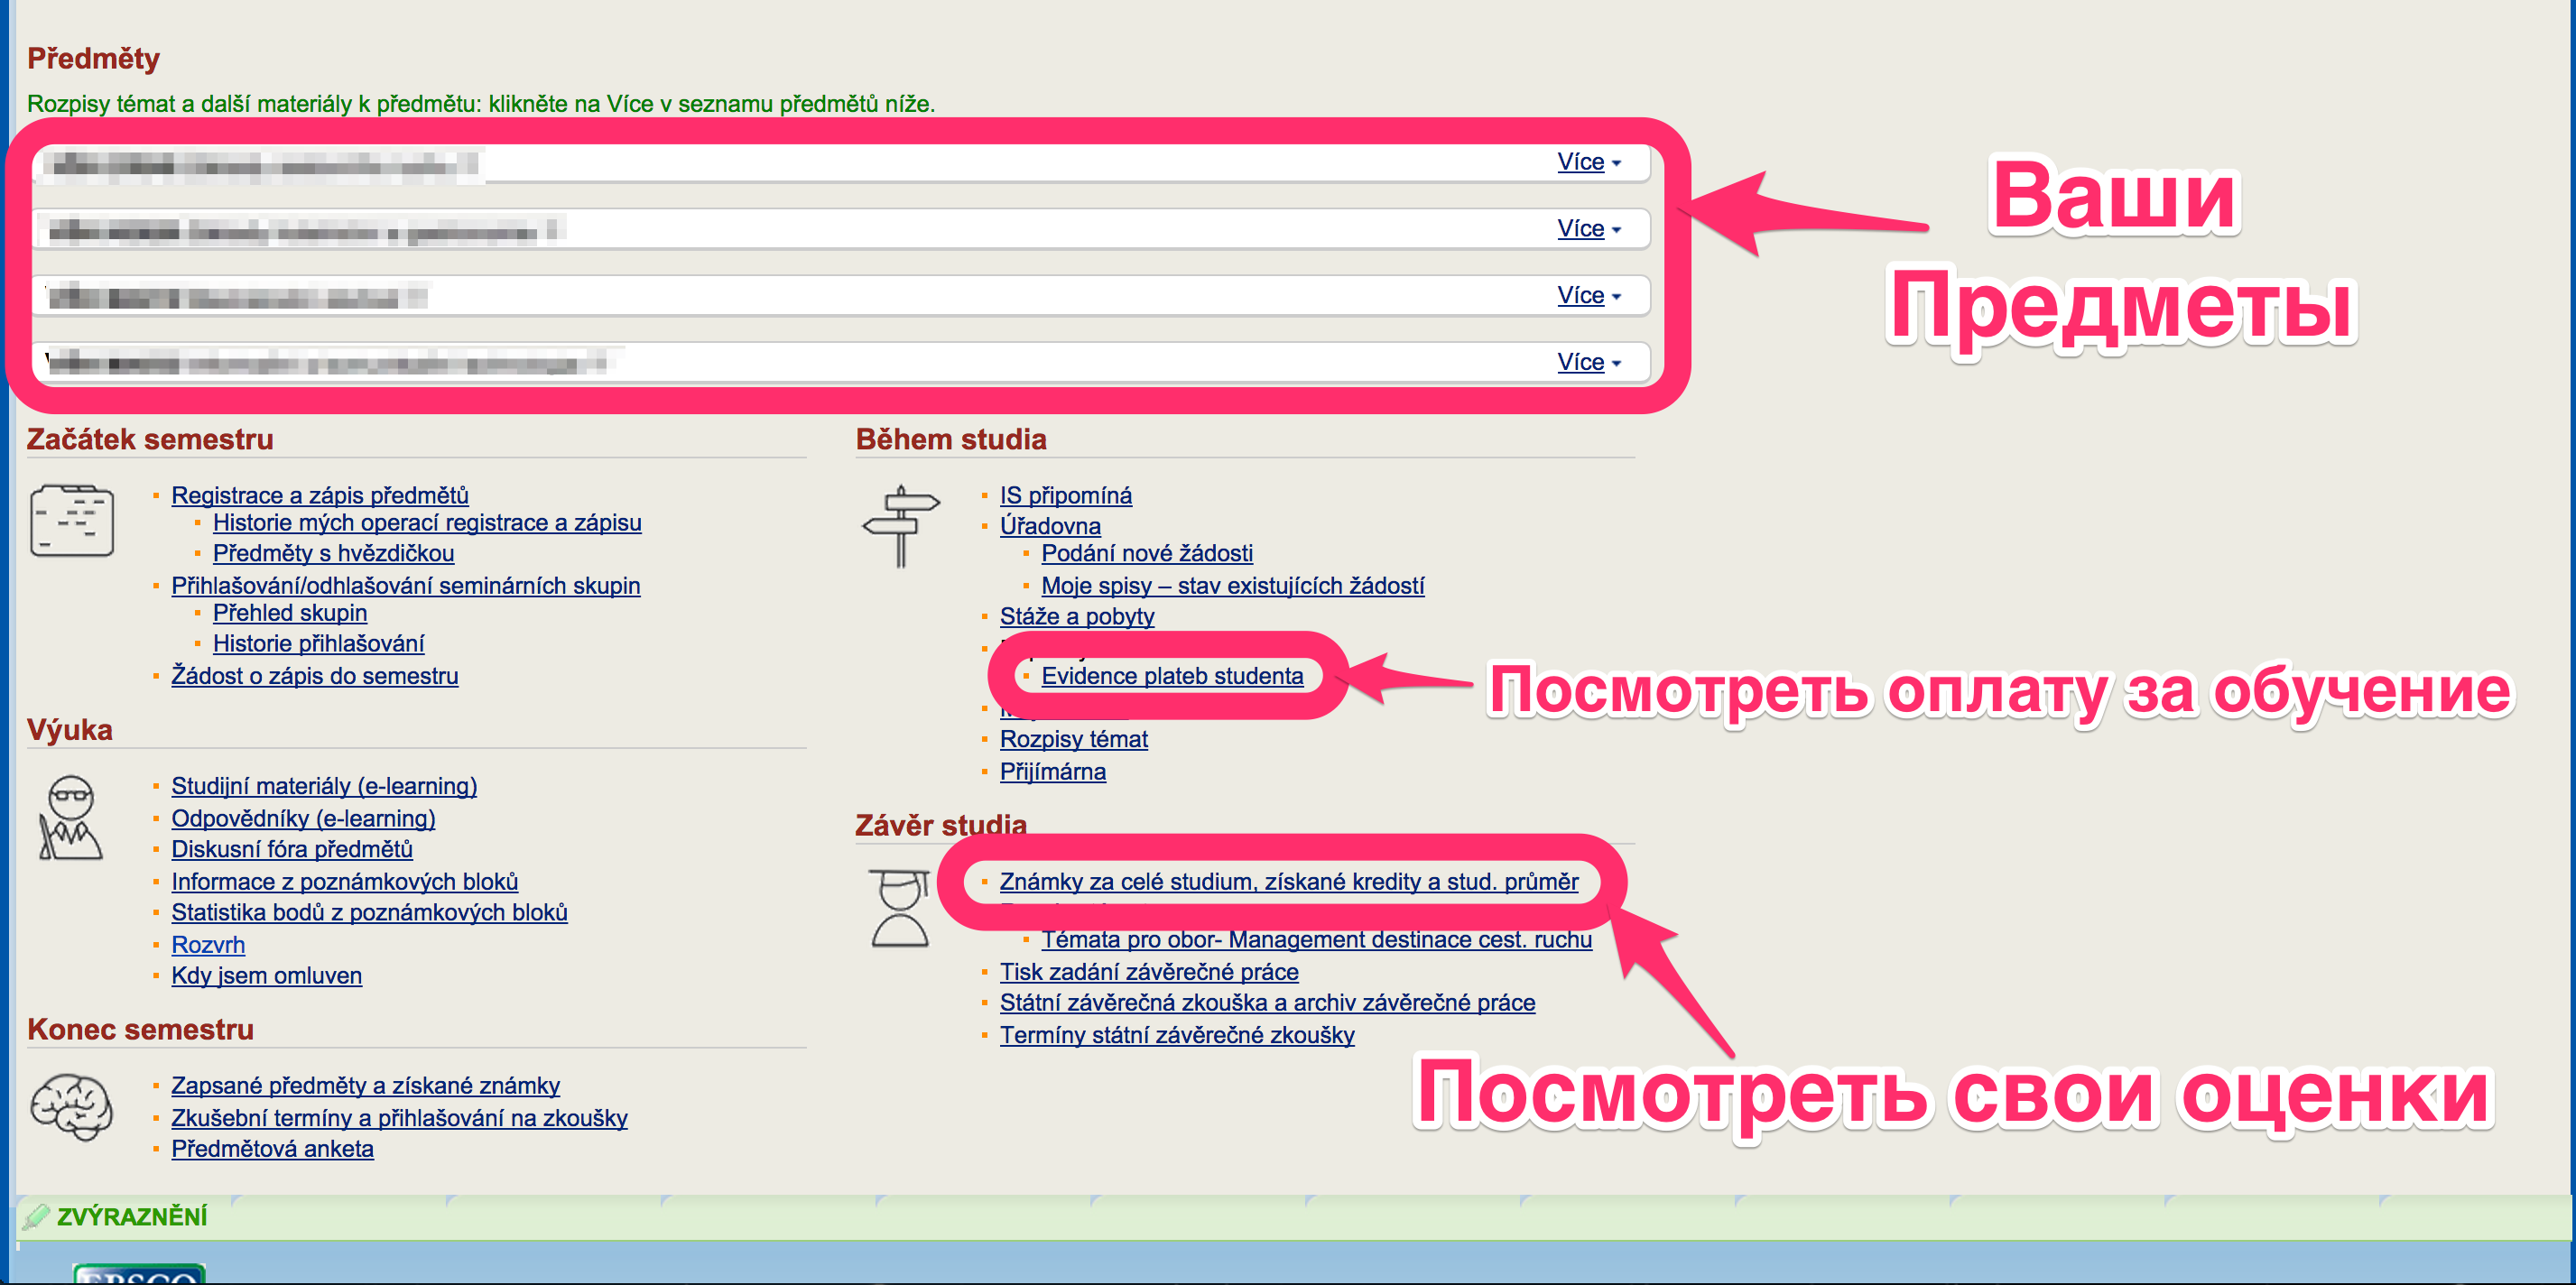
\includegraphics[width=\textwidth]{s18} \\

\newpage

Также в начале года вас могут попросить зарегистрироваться в новом учебном году в разделах
\textbf{Registrace a zápis předmětů} и \textbf{Zapsané předměty a získané známky}.

Об этом будут оповещать 
в студенческом отделении в разделе 
\textbf{Vývěska - \href{https://is.vsh.cz/auth/bb/skola/studijni/}{Studijní odd.}} \\

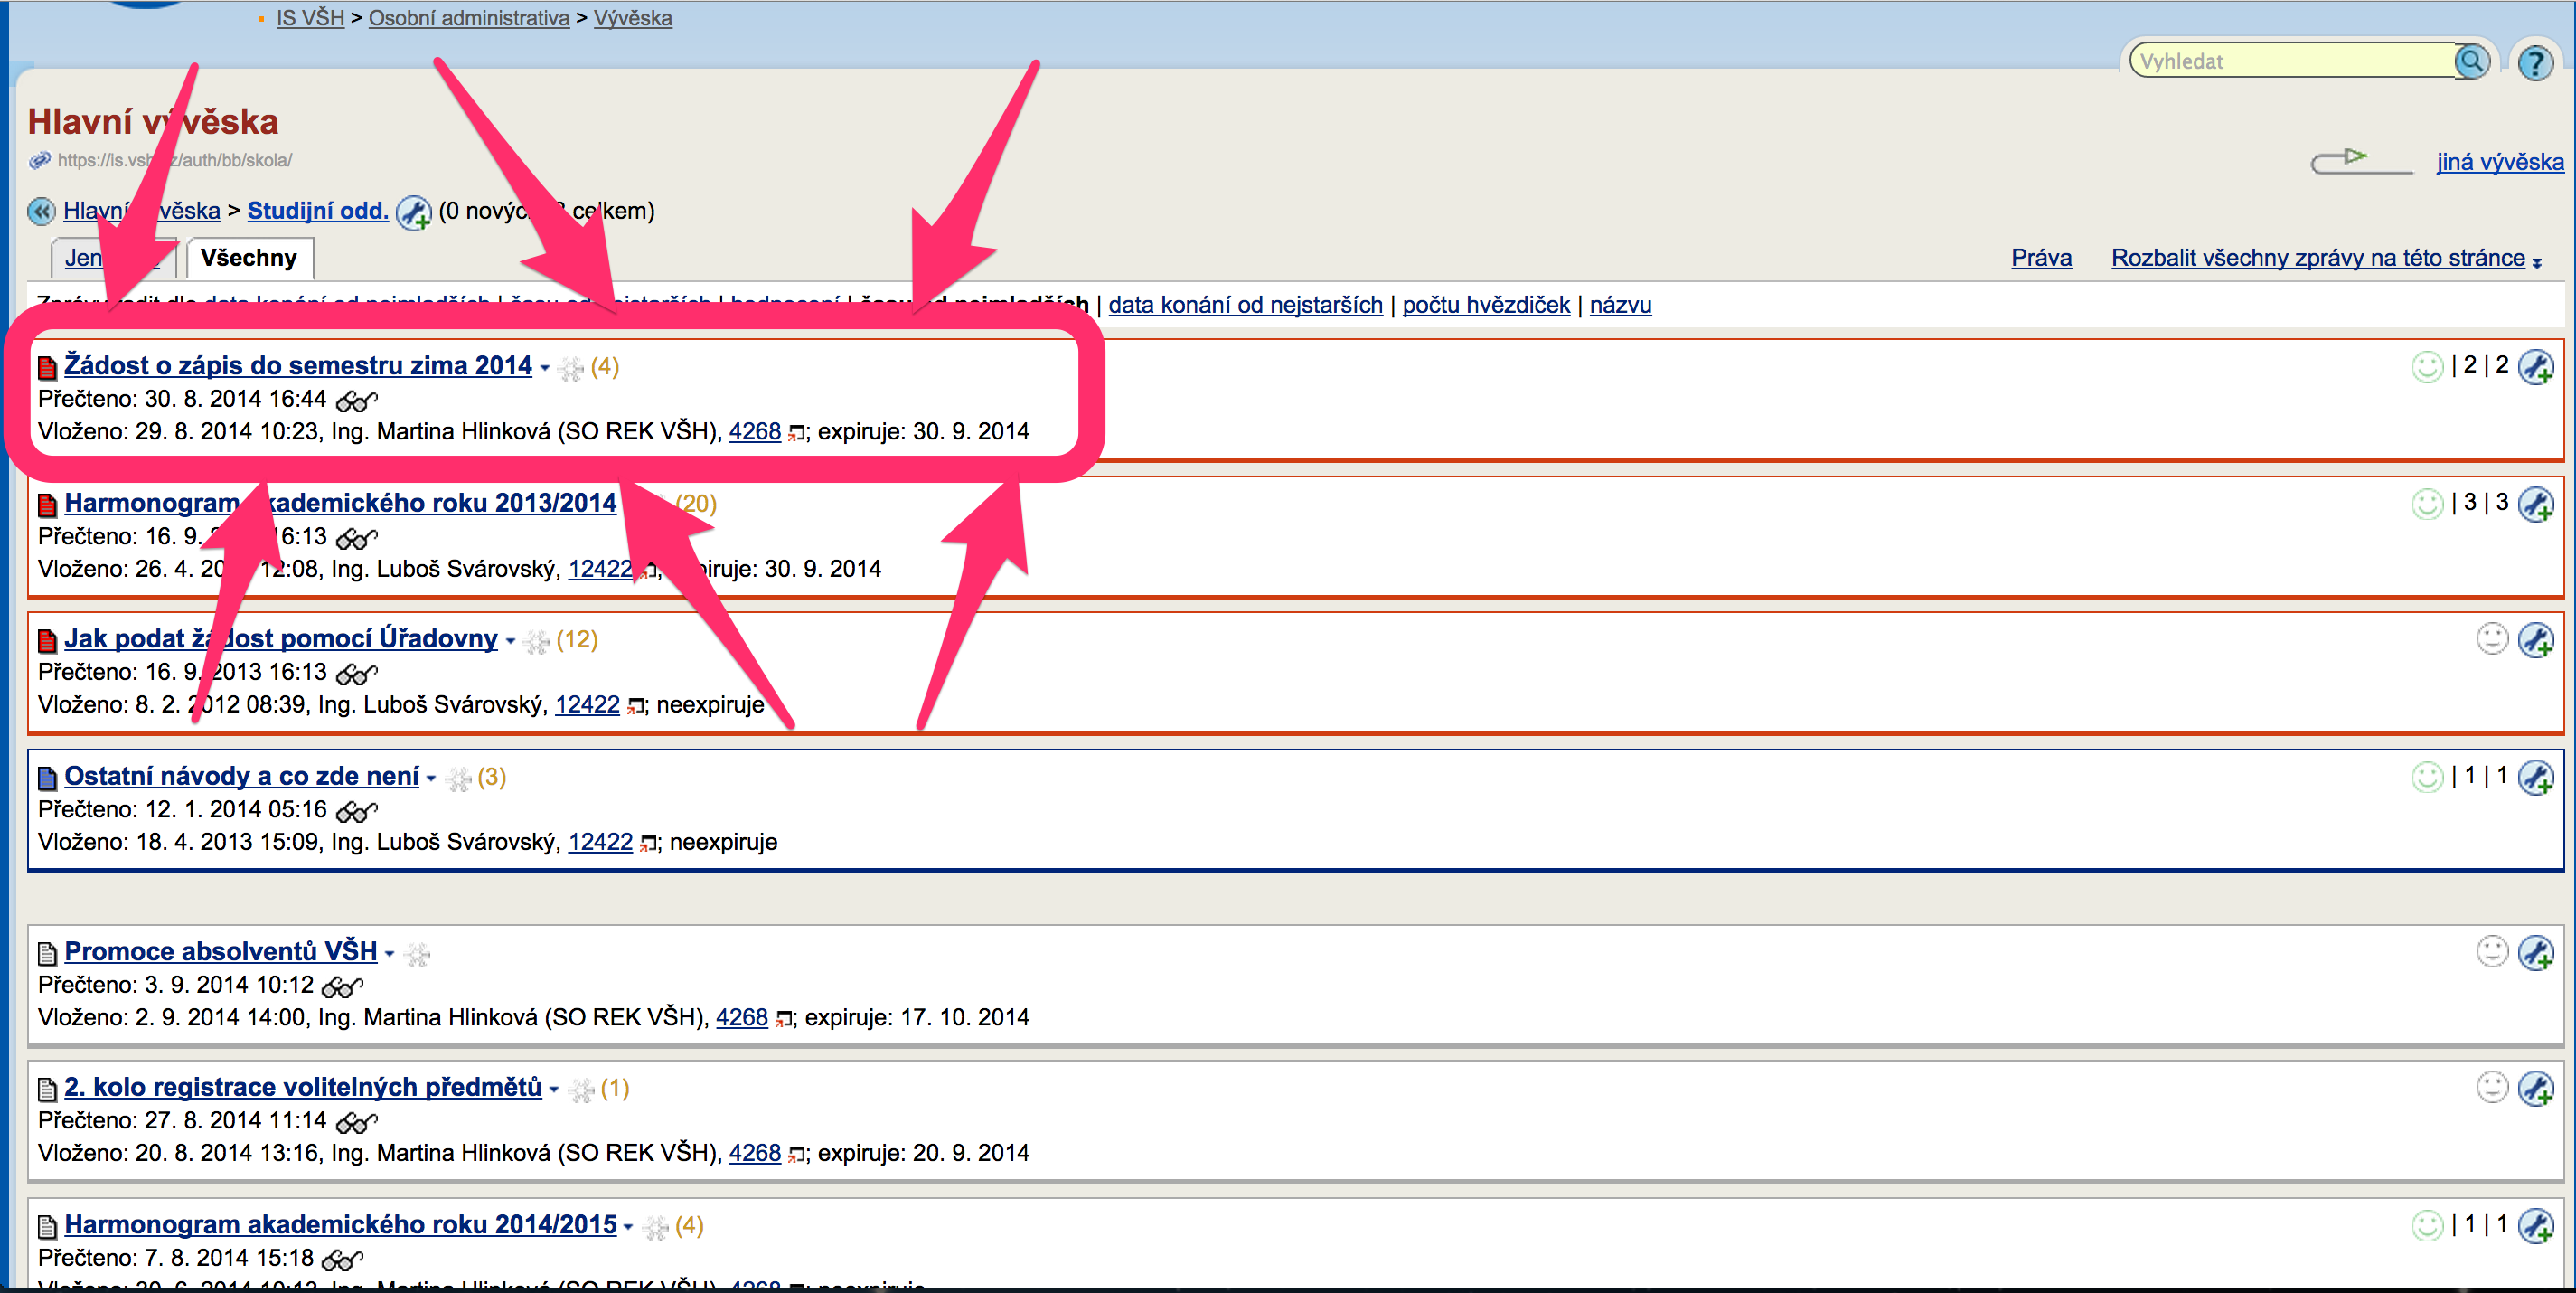
\includegraphics[width=\textwidth]{s19} \\

\newpage

\section{Поиск}

Поиск по системе осуществляется с помощью указанной на скриншоте строки
поиска и святых духов. \\

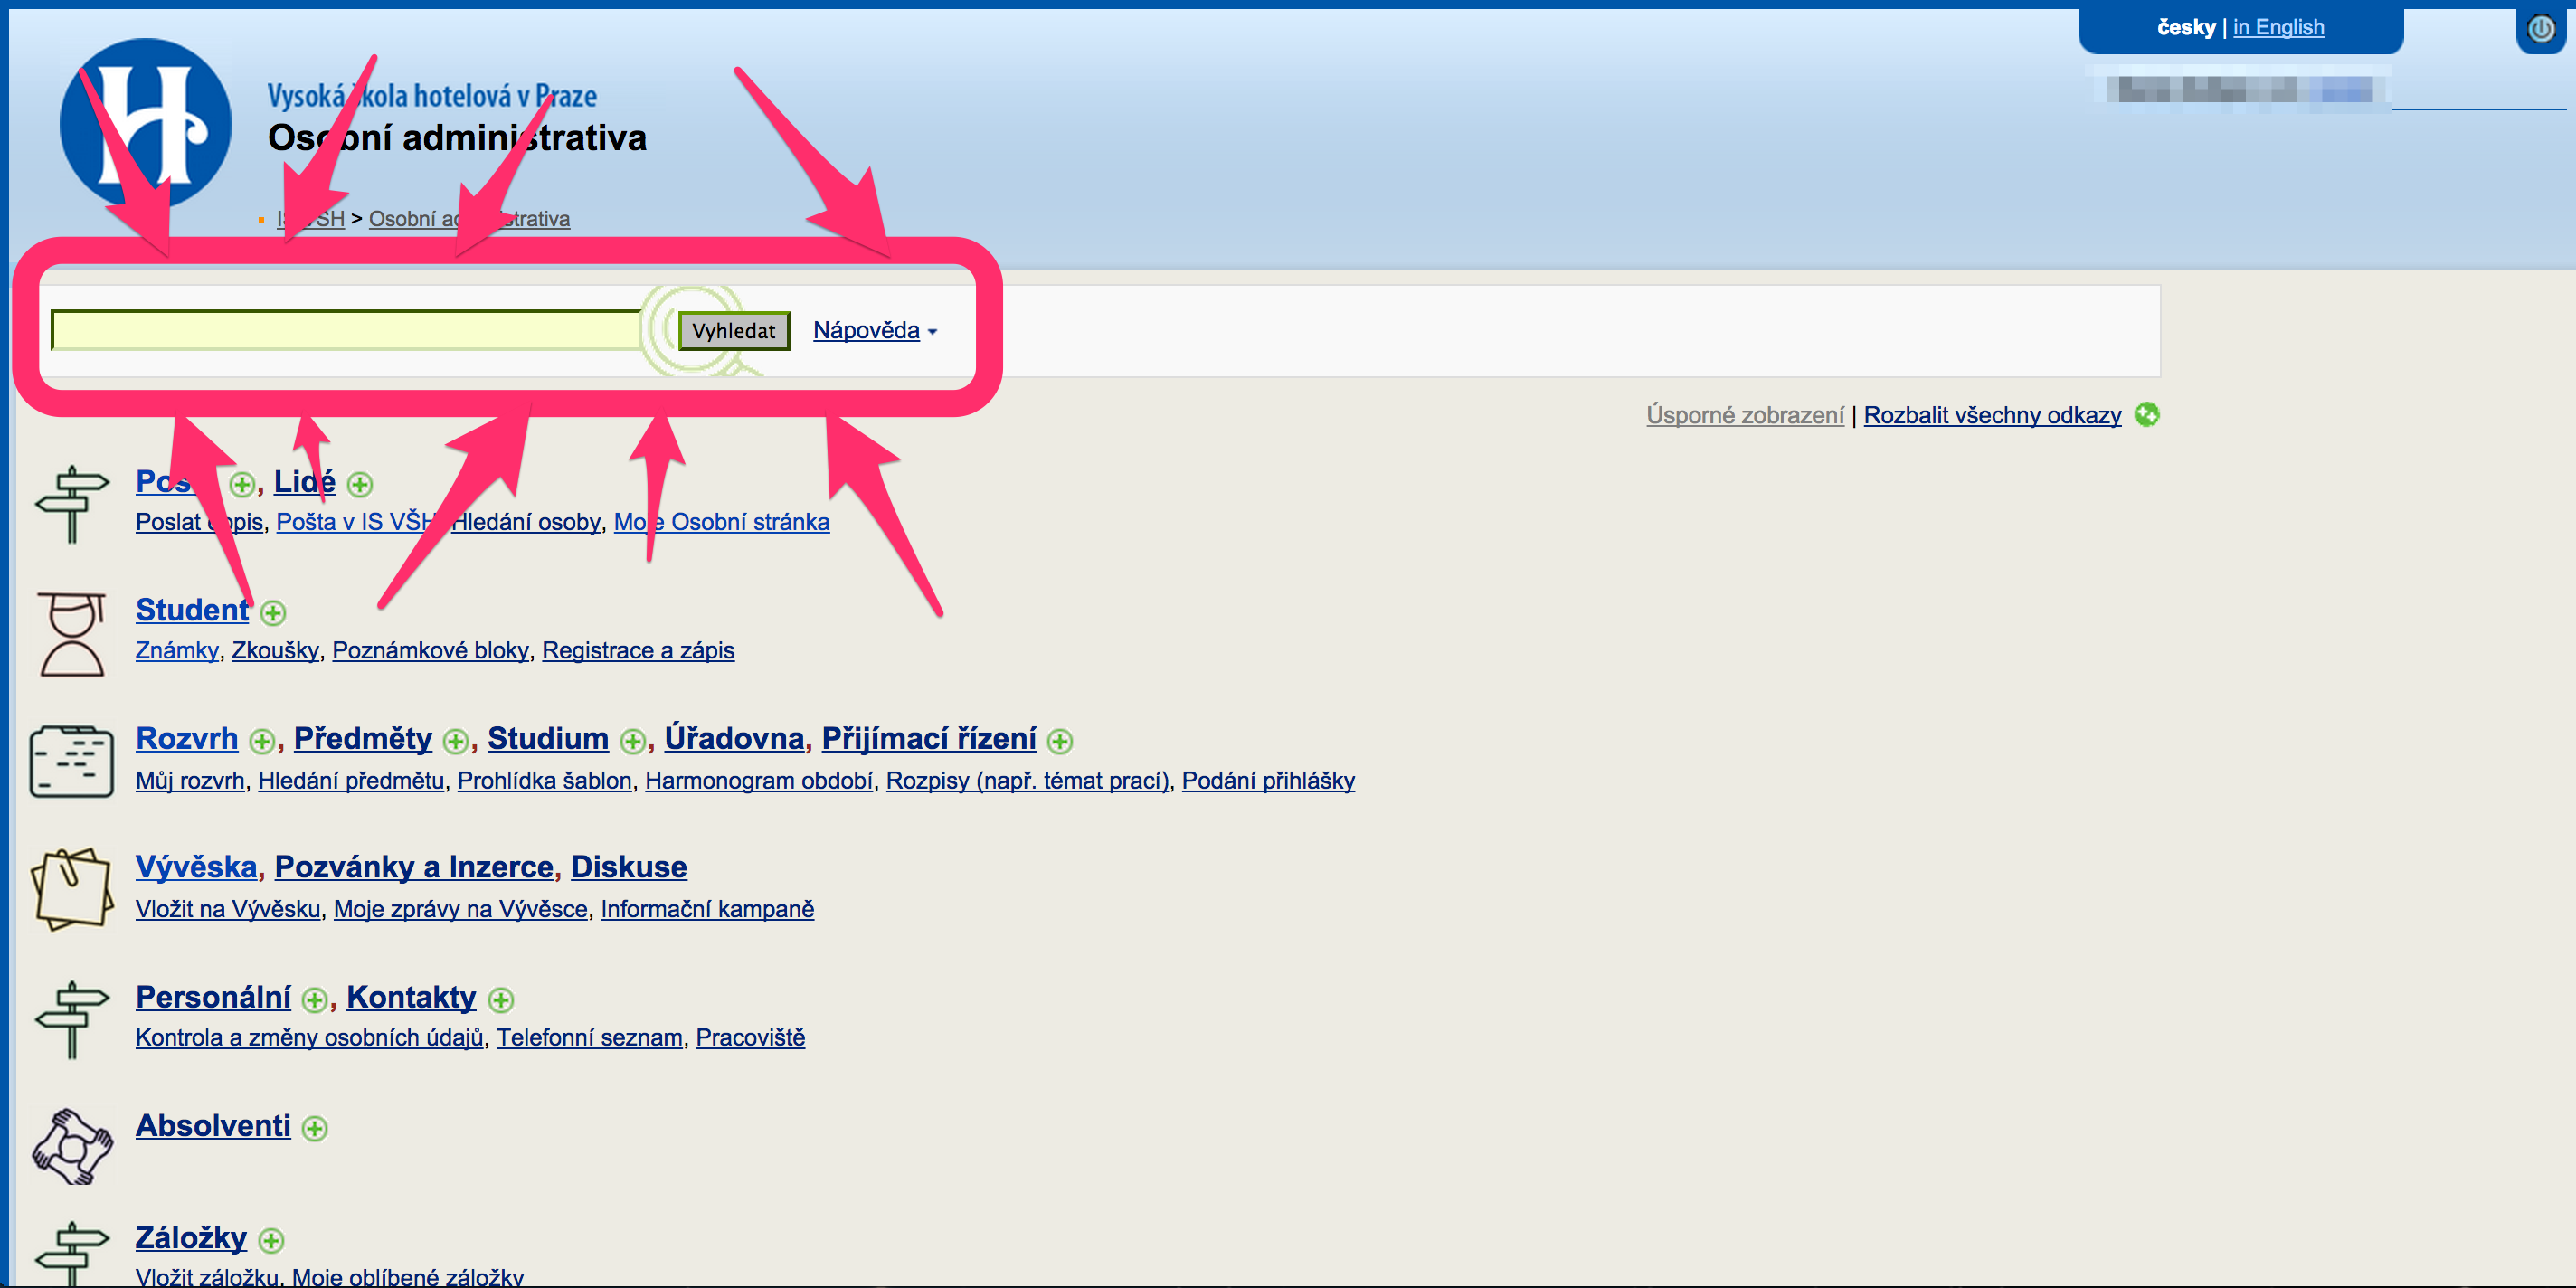
\includegraphics[width=\textwidth]{s20} \\

Достаточно вбить в строку нужное вам слово и нажать \textbf{Enter}, 
как вы перейдете на страницу результатов.

Для поиска учебных материалов, выберите раздел \textbf{Studijní materiály}. \\

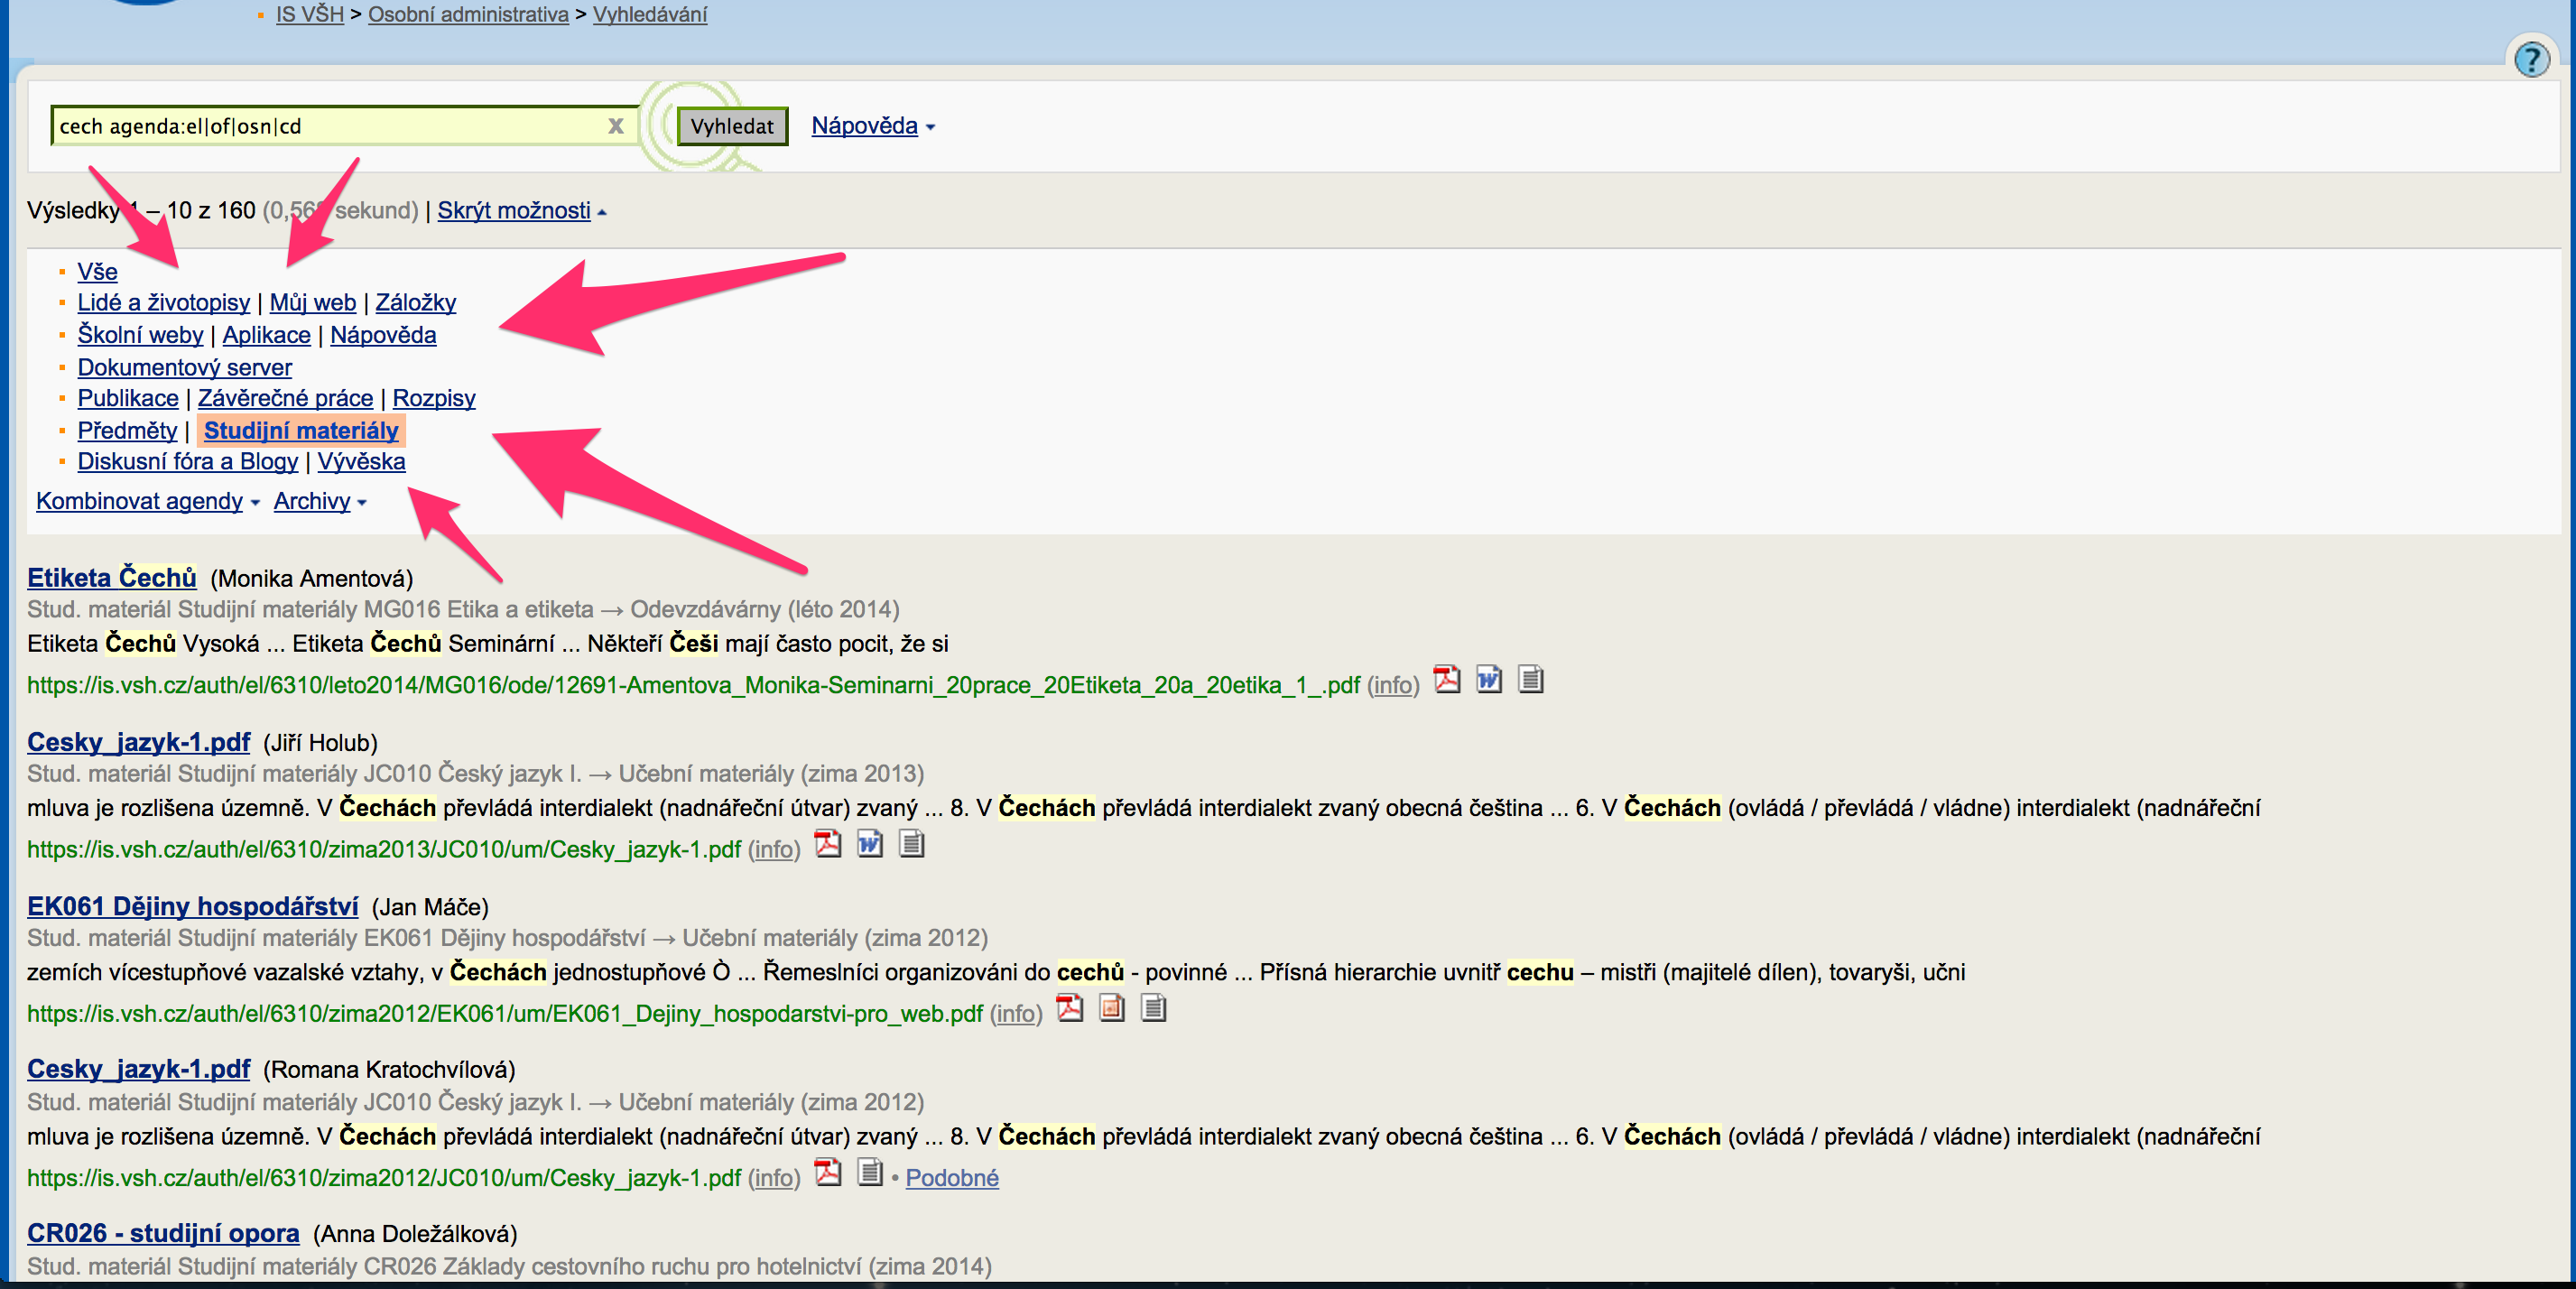
\includegraphics[width=\textwidth]{s21} \\



\newpage

\section{Заключение}

Надеюсь, что это небольшое пособие окажется для вас полезным. 
Мне было очень интересно над ним работать, несмотря на все затруднения 
и экзистенциальные кризисы.

Если вам очень понравилось, и вы хотите меня отблагодарить,
то прямо сейчас, пока вы это читаете, поднимите руки вверх, 
скажите \textbf{"Я, ЧОРТОВ БЭТМЭН!"} (да, именно через О), голосом Кристиана Бэйла, 
когда он допрашивал Бэйна в конце Dark Knight Rises, и я буду счастлив. \\

Теперь немного самопиара:

\href{http://vshub.wordpress.com}{VŠHub} - здесь я собираю все полезные материалы, 
которые могут пригодиться в нашей учебе. К сожалению, много полезного найти не удаётся.
К счастью, то, что найти не удалось, я пишу сам.

\href{https://hunfauser.github.io/usefulpage/}{Useful Page} - на этой страничке 
я разместил большую подборку полезных материалов, разширяющих кругозор (но не сознание. 
С этим не ко мне). Какие онлайн-курсы выбрать, какие расширения для браузеров установить - об 
этом, и всём остальном вы узнаете, если нажмёте на ссылку вверху.

Что же касается социальных сетей, то меня в них нет. Серьёзно! \\

Я желаю вам всего наилучшего в этой жизни. Будьте любознательными, стремитесь узнать как можно больше
и не гладьте ёжиков голыми руками. \\

\vspace{7ex}

\textbf{HOORAY!!!}

\vspace{7ex}

Напоследок, подборка фактов, \sout{которые никому не нужны}: \\
- Хан Соло стрелял первым, \\
- на моей клавиатуре отсутствуют кириллические буквы, \\
- если у вас MAC и вы хотите посмотреть Звёздные Войны, 
зайдите в программу Терминал (Terminal) и напишите telnet towel.blinkenlights.nl, \\
- Не называйте меня Дэнчиком!

\centering
\vfill
Всегда ваш, \\
Дэнчик

\end{document} % конец документа